% ThinkAlgo — Geometry and Measurement — Grade 7
% Edition: teacher (with solutions), EN.  Generated by build_grade7.py — edit body/ and rebuild.
\documentclass[11pt]{article}
\newif\ifsol \soltrue
\usepackage{iftex}
\ifPDFTeX
  \usepackage[utf8]{inputenc}\usepackage[T5]{fontenc}
\else
  \usepackage{fontspec}
\fi
\usepackage[a4paper,top=2.95cm,headheight=1.5cm,headsep=0.45cm,bottom=3.1cm,left=1.9cm,right=1.9cm]{geometry}
\usepackage{amsmath,amssymb}
\usepackage{tikz}\usetikzlibrary{calc,shadows,shapes.geometric}
\usepackage[most]{tcolorbox}
\usepackage{enumitem}
\usepackage{array}
\usepackage{tabularx}
\usepackage{colortbl}
\usepackage{comment}
\usepackage{needspace}
\usepackage{fancyhdr}
\usepackage{fontawesome5}
\usepackage{graphicx}
\usepackage{microtype}
% PDF outline (bookmarks) so each chapter shows in the reader's outline — does not change the page layout
\usepackage[hidelinks,unicode,bookmarksnumbered=false,bookmarksopen=true,bookmarksopenlevel=0]{hyperref}
\usepackage{bookmark}
\usetikzlibrary{decorations.pathreplacing,arrows.meta,angles,quotes,patterns,positioning,through,intersections}

% ---------------- palette: navy family + subtle light tint; orange ONLY in the logo ----------------
% ----- EXACT palette from the user's original main (36).tex (vivid, not pale) -----
\definecolor{tmBlue}{RGB}{66,133,244}   % problem / header / section
\definecolor{tmGreen}{RGB}{52,168,83}   % solution
\definecolor{tmOrange}{RGB}{255,152,0}  % example
\colorlet{Navy}{tmBlue}                 % header rule / section heading / badge / divider
\definecolor{NavyD}{HTML}{222222}       % solution body text (dark, readable)
\colorlet{Gold}{Navy}
\colorlet{ProbBlue}{tmBlue}             % problem boxes
\colorlet{SolGreen}{tmGreen}            % solution boxes
\definecolor{AnsRed}{HTML}{E02424}      % vivid red for answers / totals
\definecolor{CardGreen}{HTML}{34A853}   % digit-card green
\definecolor{StarGold}{HTML}{F2B134}    % difficulty star (gold)
\definecolor{KidOrange}{HTML}{DE8A2C}   % logo accent only
\definecolor{Ink}{HTML}{1F2733}       % body text
\definecolor{Slate}{HTML}{5B6A82}     % muted labels
\definecolor{Line}{HTML}{C6D0DF}      % light hairlines / student boxes
\definecolor{Tint}{HTML}{EDF1F7}      % pale panel fill (worked solution / answer)
% aliases so older names keep working
\colorlet{TextDark}{Ink}\colorlet{TextGray}{Slate}\colorlet{Soft}{Slate}
\colorlet{CardLine}{Line}\colorlet{Teal}{Navy}\colorlet{ProbB}{Navy}\colorlet{SolG}{Navy}
% bright, kid-friendly colours for bar-model (sơ đồ đoạn thẳng) blocks
\definecolor{tmPurple}{RGB}{124,77,226}
\definecolor{tmTeal}{RGB}{0,150,136}
\definecolor{tmPink}{RGB}{233,30,99}
\AtBeginDocument{\color{Ink}}
\raggedbottom  % natural flow, even spacing (no stretched gaps)
\setlength{\parindent}{0pt}\setlength{\parskip}{0.18em}
\renewcommand{\arraystretch}{1.35}
\providecommand{\AnsWord}{Đáp số}

% ---------------- brand logo (original mark) ----------------
\newcommand{\logomark}[1]{\begin{tikzpicture}[baseline=-0.55ex,scale=#1]
  \draw[KidOrange,line width=1.5pt] (-0.27,0) .. controls (-0.27,0.23) and (0,0.23) .. (0,0)
        .. controls (0,-0.23) and (-0.27,-0.23) .. (-0.27,0);
  \draw[Navy,line width=1.5pt] (0.27,0) .. controls (0.27,0.23) and (0,0.23) .. (0,0)
        .. controls (0,-0.23) and (0.27,-0.23) .. (0.27,0);
\end{tikzpicture}}
% real brand logo image (gold infinity + "think algo" wordmark)
\newcommand{\logohead}{\IfFileExists{logo.png}{\includegraphics[height=1.35cm]{logo.png}}%
  {\raisebox{0.35cm}{\logomark{1.5}\hspace{0.5em}{\Large\bfseries\color{KidOrange}think\,\color{Navy}algo}}}}

% ---------------- running header (logo + Name/Date + topic) on EVERY page, single navy rule ----------------
\pagestyle{fancy}\fancyhf{}
\renewcommand{\headrulewidth}{1.4pt}\renewcommand{\footrulewidth}{0pt}
\renewcommand{\headrule}{{\color{Navy}\hrule height 1.3pt}}
\fancyhead[L]{\raisebox{-0.95cm}{\logohead}}
\fancyhead[R]{\setlength{\tabcolsep}{0pt}%
  \begin{tabular}{@{}r@{}}
    {\small\color{Ink}{\color{tmBlue}\faUserEdit}~\NameWord:~\rule{3.0cm}{0.5pt}\quad{\color{tmBlue}\faCalendarDay}~\DateWord:~\rule{1.9cm}{0.5pt}}\\[5pt]
    {\large\bfseries\color{Navy}\CurTopic}
  \end{tabular}}

% ---------------- footer (rounded page border + Topic/Grade + thinkalgo.com + page + tagline) ----------------
% NOTE: a remember-picture overlay must be placed DIRECTLY in \fancyfoot, NOT inside \def/\newcommand.
\fancyfoot[C]{\begin{tikzpicture}[remember picture, overlay]
  \draw[Navy!40, line width=1.4pt, rounded corners=12pt]
     ($(current page.north west)+(0.8cm,-0.8cm)$) rectangle ($(current page.south east)+(-0.8cm,0.45cm)$);
  \coordinate (FL) at ($(current page.south west)+(1.2cm, 2.18cm)$);
  \coordinate (FR) at ($(current page.south east)+(-1.2cm, 2.18cm)$);
  \draw[Navy!55, line width=1pt] (FL) -- (FR);
  \node[fill=white, draw=Navy, line width=1.2pt, rounded corners=8pt, font=\bfseries\small,
        text=Navy, inner xsep=11pt, inner ysep=4pt] at ($(current page.south)+(0,2.18cm)$) {{\color{tmBlue}\faGlobe}\ \ thinkalgo.com};
  \node[text=Slate, font=\footnotesize, anchor=north west, align=left, inner sep=0pt, text width=7.6cm]
        at ($(FL)+(0.1cm,-0.30cm)$) {{\color{tmBlue}\faTag}\ \TopicWord: \textbf{\color{Ink}\CurTopic}\\[1.5pt]{\color{tmBlue}\faGraduationCap}\ \DocGrade};
  \node[text=Slate, font=\footnotesize] at ($(current page.south)+(0,1.20cm)$) {\thepage};
  \node[text=Slate, font=\scriptsize, anchor=north east, align=right, inner sep=0pt, text width=7.4cm]
        at ($(FR)+(-0.1cm,-0.34cm)$) {{\normalsize\bfseries\color{Navy}ThinkAlgo}\ — From Math Thinking to Code};
\end{tikzpicture}}

% ---------------- page-1 lead-in (topic is already in the header; keep a slim spacer) ----------------
\newcommand{\titlehead}{\vspace*{-0.2cm}}
\providecommand{\CurTopic}{}

% chapter banner + sets the running-header topic. #1 = number, #2 = title
\newcommand{\chapterhead}[2]{\renewcommand{\CurTopic}{#2}%
  \setcounter{seccnt}{0}% each chapter is independent: section badges restart at 1
  \phantomsection\pdfbookmark[0]{#1. #2}{chap#1}\label{chap:#1}% add this chapter to the PDF outline + TOC ref
  \par\vspace{0.1cm}\noindent\begin{tikzpicture}[baseline=-0.5ex]
    \node[circle,fill=tmBlue,text=white,font=\Large\bfseries,minimum size=0.95cm,inner sep=0pt](cn){#1};
    \node[anchor=west,font=\LARGE\bfseries,text=tmBlue] at ([xshift=12pt]cn.east){#2};
  \end{tikzpicture}\par\vspace{4pt}\noindent\textcolor{tmBlue}{\rule{\linewidth}{2pt}}\par\vspace{0.5cm}}

% ---------------- section heading (outline navy number badge, no fill) ----------------
\newcounter{seccnt}
\newcommand{\shead}[1]{\par\vspace{0.7em}\refstepcounter{seccnt}%
  \noindent
\begin{tikzpicture}[baseline=-0.6ex]
    \node[circle,draw=Gold,line width=1.2pt,text=Gold,font=\bfseries,minimum size=1.05em,inner sep=1pt]{\theseccnt};
  \end{tikzpicture}\hspace{0.4em}{\large\bfseries\color{Navy} #1}\par\vspace{0.25em}}

% ============ boxes EXACTLY per the original main (36).tex: solid-blue PROBLEM, solid-orange EXAMPLE,
%              outline-green SOLUTION, all with drop shadow + rounded corners ============
% ---------------- knowledge box: white, tmBlue border + left accent + drop shadow ----------------
\newtcolorbox{knowbox}{enhanced,breakable,colback=white,colframe=tmBlue!70,boxrule=0.9pt,arc=5pt,
  left=12pt,right=11pt,top=6pt,bottom=6pt,drop shadow,
  borderline west={3.5pt}{0pt}{tmBlue}}

% ---------------- EXAMPLE (Ví dụ): SOLID ORANGE tab, white text ----------------
\newtcolorbox{exbox}[1]{enhanced,breakable,colback=white,colframe=tmOrange,boxrule=1pt,arc=5pt,
  left=12pt,right=11pt,top=14pt,bottom=7pt,drop shadow,
  attach boxed title to top left={xshift=10pt,yshift=-\tcboxedtitleheight/2},
  boxed title style={colback=tmOrange,colframe=tmOrange,arc=4pt,boxrule=0pt,drop shadow},
  title={#1},fonttitle=\bfseries\color{white}}
\newcommand{\guide}{\par\vspace{2pt}{\bfseries\color{tmBlue}\GuideWord}\par\nopagebreak}

% ---------------- PROBLEM (Bài): SOLID BLUE tab, white text ----------------
\newtcolorbox{probbox}[2]{enhanced,breakable,colback=white,colframe=tmBlue,boxrule=1pt,arc=5pt,
  left=12pt,right=10pt,top=14pt,bottom=7pt,drop shadow,
  attach boxed title to top left={xshift=10pt,yshift=-\tcboxedtitleheight/2},
  boxed title style={colback=tmBlue,colframe=tmBlue,arc=4pt,boxrule=0pt,drop shadow},
  fonttitle=\bfseries\color{white},title={\ProbWord\ #1\ifx\relax#2\relax\else#2\fi}}

% ---------------- SOLUTION (Lời giải): OUTLINE GREEN tab (white fill, green border + text) ----------------
% Teacher: a green tcolorbox. Student: the body is dropped entirely (comment pkg — robust with tables/\\).
\ifsol
  \newtcolorbox{solbox}{enhanced,breakable,colback=white,colframe=tmGreen,boxrule=1pt,arc=5pt,
    left=12pt,right=10pt,top=14pt,bottom=7pt,drop shadow,
    attach boxed title to top left={xshift=10pt,yshift=-\tcboxedtitleheight/2},
    boxed title style={colback=white,colframe=tmGreen,boxrule=1pt,arc=4pt,drop shadow},
    fonttitle=\bfseries\color{tmGreen!88!black},title={\SolTitle},before upper={\color{NavyD}}}
\else
  \excludecomment{solbox}
\fi

% ---------------- answer highlight: label green, value RED ----------------
\newcommand{\ans}[1]{\par\smallskip{\bfseries\color{tmGreen!88!black}\AnsWord:}\ {\bfseries\color{AnsRed}#1}\par}

% ---------------- digit cards (exact original style: fill=c!10, border=c!60!black, drop shadow) ----------------
% \digitcards{0/gray,1/cyan,2/green,3/cyan} : value/colour pairs
\newcommand{\digitcards}[1]{\begin{center}\begin{tikzpicture}[scale=0.7,transform shape,font=\sffamily]
  \def\dx{0}\foreach \v/\c in {#1}{
    \node[draw=\c!60!black,line width=1.5pt,fill=\c!10,rounded corners=4pt,
          minimum width=1cm,minimum height=1.4cm,drop shadow] at (\dx,0){\Huge\bfseries \v};
    \pgfmathsetmacro\dx{\dx+1.5}\xdef\dx{\dx}}
\end{tikzpicture}\end{center}}

% ---------------- student working space (white, light border) ----------------
\newcommand{\worksp}[1]{\ifsol\else\begin{tcolorbox}[colback=white,colframe=Line,boxrule=0.8pt,
  arc=5pt,height=\dimexpr#1+0.05cm\relax,left=8pt,right=8pt,top=4pt,bottom=4pt]{\footnotesize\color{Slate}\itshape\WorkWord}\end{tcolorbox}\fi}

% ---------------- \probsol{solution} : Teacher shows the green solution box; Student shows a BLANK
%   "Bài làm" box whose height matches that solution's height (writing room = work needed), so both
%   versions have identical per-problem height and paginate the same. ----------------
\newsavebox{\solmeasure}\newlength{\solht}
\newcommand{\probsol}[1]{%
  \begin{lrbox}{\solmeasure}\begin{minipage}{\dimexpr\linewidth-24pt\relax}#1\end{minipage}\end{lrbox}%
  \ifsol
    \begin{solbox}#1\end{solbox}%
  \else
    \setlength{\solht}{\dimexpr\ht\solmeasure+\dp\solmeasure+0.85cm\relax}%
    \ifdim\solht<1.35cm\setlength{\solht}{1.35cm}\fi
    \ifdim\solht>\StudentMaxWork\setlength{\solht}{\StudentMaxWork}\fi
    \begin{tcolorbox}[colback=white,colframe=Line,boxrule=0.8pt,arc=5pt,
      left=8pt,right=8pt,top=4pt,bottom=4pt,height=\solht]{\footnotesize\color{Slate}\itshape\WorkWord}\end{tcolorbox}%
  \fi}

% ---------------- practice divider: blue left accent bar, no fill ----------------
\newcommand{\dividerbar}[1]{\par\vspace{0.6em}\noindent
  \begin{tcolorbox}[enhanced,frame hidden,interior hidden,borderline west={5pt}{0pt}{ProbBlue},
    colback=white,left=12pt,right=12pt,top=5pt,bottom=5pt,arc=4pt]
  {\large\bfseries\color{ProbBlue} #1}\end{tcolorbox}\vspace{0.4em}}

% place-value choice-count diagram (Cambridge style): #1 = "label/count/note/color" list, #2 = result
% notes must NOT contain commas or slashes (they separate \foreach fields)
\newcommand{\countboxes}[2]{\begin{center}\begin{tikzpicture}[scale=0.62,transform shape,font=\sffamily]
  \def\xx{0}%
  \foreach \lab/\cnt/\note/\col [count=\i] in {#1}{%
    \ifnum\i>1\relax \node[text=gray,font=\Huge] at (\xx-1.8,0){$\times$};\fi
    \node[draw=\col!65,fill=\col!8,rounded corners=3pt,line width=1pt,minimum width=2.7cm,minimum height=1.7cm] at (\xx,0){};
    \node[text=\col!85,font=\bfseries] at (\xx,0.58){\lab};
    \node[text=\col!88,font=\Huge\bfseries] at (\xx,-0.1){\cnt};
    \node[text=gray,font=\scriptsize] at (\xx,-1.05){\note};
    \pgfmathsetmacro\xx{\xx+3.6}\xdef\xx{\xx}}%
  \node[text=gray,font=\Huge] at (\xx-1.8,0){$=$};
  \node[text=red,font=\Huge\bfseries] at (\xx,0){#2};
\end{tikzpicture}\end{center}}

% ======== bar model (sơ đồ đoạn thẳng): lightly-rounded blocks, darker border, tiny gaps, bright colours ========
% one block: \blk{x1}{x2}{yc}{height}{colour}{label}  (a small gap is left on each side)
\newcommand{\blk}[6]{%
  \draw[rounded corners=1.3pt,fill=#5!16,draw=#5!80!black,line width=1pt]
    (#1+0.045,#3-#4/2) rectangle (#2-0.045,#3+#4/2);
  \node[font=\small\bfseries,text=#5!52!black] at ({(#1+#2)/2},#3){#6};}
% measurement with a double-headed ARROW (not a brace) + label above the span: \brcup{x1}{x2}{y}{label}
\newcommand{\brcup}[4]{%
  \draw[<->,>=stealth,tmBlue!72!black,line width=0.7pt] (#1+0.05,#3)--(#2-0.05,#3);
  \node[above=-1.5pt,font=\footnotesize,text=tmBlue!58!black] at ({(#1+#2)/2},#3){#4};}
% measurement with a double-headed ARROW + label below the span: \brcdn{x1}{x2}{y}{label}
\newcommand{\brcdn}[4]{%
  \draw[<->,>=stealth,tmBlue!72!black,line width=0.7pt] (#1+0.05,#3)--(#2-0.05,#3);
  \node[below=-1.5pt,font=\footnotesize,text=tmBlue!58!black] at ({(#1+#2)/2},#3){#4};}
% row label at the left of a bar: \rowlab{x}{y}{text}
\newcommand{\rowlab}[3]{\node[anchor=east,font=\small\bfseries,text=Ink] at (#1,#2){#3};}
% vertical right-pointing CURLY BRACE spanning two stacked bars: \vbrace{x}{ytop}{ybot}{label}
\newcommand{\vbrace}[4]{%
  \pgfmathsetmacro\ym{(#2+#3)/2}%
  \draw[tmBlue!72!black,line width=0.9pt,line cap=round]
    (#1,#2) .. controls (#1+0.18,#2) and (#1+0.18,#2-0.18) .. (#1+0.18,#2-0.22)
    -- (#1+0.18,{\ym+0.22})
    .. controls (#1+0.18,\ym) and (#1+0.30,{\ym+0.08}) .. (#1+0.42,\ym)
    .. controls (#1+0.30,{\ym-0.08}) and (#1+0.18,\ym) .. (#1+0.18,{\ym-0.22})
    -- (#1+0.18,#3+0.22)
    .. controls (#1+0.18,#3+0.18) and (#1+0.18,#3) .. (#1,#3);
  \node[right=4pt,font=\footnotesize,text=tmBlue!58!black] at (#1+0.42,\ym){#4};}
% blank 3x3 grid for a problem statement (student fills it in)
\newcommand{\blankgrid}{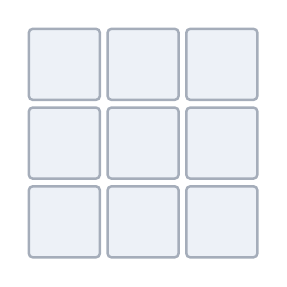
\begin{tikzpicture}[font=\sffamily]
  \foreach \r in {0,1,2}{\foreach \c in {0,1,2}{
    \draw[rounded corners=1.3pt,fill=Tint,draw=Slate!55,line width=0.9pt]
      (\c+0.05,\r+0.05) rectangle (\c+0.95,\r+0.95);}}
\end{tikzpicture}}
% wrapper: LEFT-aligned (not centred), a little air above/below
\newenvironment{barfig}{\par\vspace{3pt}\noindent\kern0.35cm\begin{tikzpicture}[font=\sffamily,>=stealth]}%
  {\end{tikzpicture}\par\vspace{3pt}}
% wrapper: CENTRED (for illustrative diagrams in theory / examples)
\newenvironment{barfigC}{\par\vspace{3pt}\begin{center}\begin{tikzpicture}[font=\sffamily,>=stealth]}%
  {\end{tikzpicture}\end{center}\vspace{2pt}}

% ---------------- difficulty stars (nicely drawn) : \stars{1}=hard, \stars{2}=very hard ----------------
\newcommand{\diffstar}{\tikz[baseline=-0.55ex]{\node[star,star points=5,star point ratio=0.46,
  draw=StarGold!72!black,fill=StarGold,line width=0.3pt,inner sep=1.75pt]{};}}
\newcommand{\stars}[1]{\ifcase#1\or\kern2pt\diffstar\or\kern2pt\diffstar\kern1.5pt\diffstar\fi}

\newcommand{\nd}[1]{\overline{#1}}

% number line: #1 last index, #2 ticks "i/label", #3 open (excluded) indices, #4 filled (solution) indices
\newcommand{\numlinex}[4]{\begin{center}\begin{tikzpicture}[x=1.55cm,>=stealth]
  \draw[->,thick,Navy](-0.45,0)--(#1+0.45,0);
  \foreach \i/\lab in {#2}{\draw[Navy,line width=0.8pt](\i,0.08)--(\i,-0.08);
     \node[below,font=\small,text=Ink]at(\i,-0.1){\lab};}
  \foreach \i in {#3}{\draw[Navy,fill=white,line width=1pt](\i,0)circle(2.3pt);}
  \foreach \i in {#4}{\fill[KidOrange](\i,0)circle(2.7pt);}
\end{tikzpicture}\end{center}}


% ======================================================================
% Grade 7 additions (shared by all four editions)
% ======================================================================
% student edition: blank "work" box height = min(solution height, this cap)
\newlength{\StudentMaxWork}\setlength{\StudentMaxWork}{7.5cm}

% ThinkAlgo tip box (label set per language by \TipWord)
\newtcolorbox{tipbox}{enhanced,breakable,colback=StarGold!8,colframe=StarGold!75!black,boxrule=1pt,arc=4pt,
  left=11pt,right=10pt,top=6pt,bottom=6pt,
  before upper={\textbf{\color{StarGold!65!black}\faLightbulb\ \TipWord}\ }}

% "Recall" box: re-states a piece of theory inside a solution / example
\newtcolorbox{recallbox}{enhanced,breakable,colback=tmBlue!5,colframe=tmBlue!45,boxrule=0.6pt,arc=3pt,
  left=8pt,right=8pt,top=4pt,bottom=4pt,
  before upper={\textbf{\color{tmBlue!80!black}\faBookOpen\ \RecallWord}\ }}

% "Why is it true? / Proof" box
\newtcolorbox{proofbox}{enhanced,breakable,colback=tmPurple!4,colframe=tmPurple!45,boxrule=0.6pt,arc=3pt,
  left=8pt,right=8pt,top=4pt,bottom=4pt,
  before upper={\textbf{\color{tmPurple!85!black}\faSearch\ \ProofWord}\ },
  after upper={\hfill$\square$}}

% "Common mistake" box
\newtcolorbox{warnbox}{enhanced,breakable,colback=AnsRed!4,colframe=AnsRed!45,boxrule=0.6pt,arc=3pt,
  left=8pt,right=8pt,top=4pt,bottom=4pt,
  before upper={\textbf{\color{AnsRed!85!black}\faExclamationTriangle\ \WarnWord}\ }}

% "Note for parents" box (short hint on how to explain the idea at home)
\newtcolorbox{parentbox}{enhanced,breakable,colback=tmTeal!5,colframe=tmTeal!50,boxrule=0.6pt,arc=3pt,
  left=8pt,right=8pt,top=4pt,bottom=4pt,
  before upper={\textbf{\color{tmTeal!80!black}\faUsers\ \ParentWord}\ }}

% numbered step inside a solution:  \step{1}{Short title}  -> "Bước 1. Short title"
\newcommand{\step}[2]{\par\smallskip\noindent{\bfseries\color{tmBlue!85!black}\StepWord~#1.}\ {\bfseries #2}\par\nopagebreak}
% verification line:  \verify{...}
\newcommand{\verify}[1]{\par\smallskip\noindent{\bfseries\color{tmGreen!80!black}\faCheckCircle\ \CheckWord}\ #1\par}

% multiple-choice options
% \choices{..}{..}{..}{..}{..}      : five short options on one line
% \choicesII{..}{..}{..}{..}{..}    : two/three per line (medium length)
% \choicesL{..}{..}{..}{..}{..}     : one option per line (long text)
\newcommand{\choices}[5]{\par\smallskip\noindent
  \begin{tabularx}{\linewidth}{@{}XXXXX@{}}(A)\ #1&(B)\ #2&(C)\ #3&(D)\ #4&(E)\ #5\end{tabularx}\par}
\newcommand{\choicesII}[5]{\par\smallskip\noindent
  \begin{tabularx}{\linewidth}{@{}XXX@{}}(A)\ #1&(B)\ #2&(C)\ #3\\(D)\ #4&(E)\ #5&\end{tabularx}\par}
\newcommand{\choicesL}[5]{\par\smallskip\noindent
  \begin{tabular}{@{}l@{}}(A)\ #1\\(B)\ #2\\(C)\ #3\\(D)\ #4\\(E)\ #5\end{tabular}\par}

% centred figure inside a problem / solution
\newenvironment{figC}{\par\vspace{2pt}\begin{center}\begin{tikzpicture}[font=\sffamily\small,>=stealth,line join=round]}%
  {\end{tikzpicture}\end{center}\vspace{1pt}}

\def\DocGrade{Grade 7}
\def\ProbWord{Problem}
\def\SolWord{Solution.}
\def\GuideWord{Guided solution.}
\def\PageWord{Page}
\def\NameWord{Name}
\def\DateWord{Date}
\def\SolTitle{Detailed solution}
\def\WorkWord{Your work:}
\def\TopicWord{Topic}
\def\AnsWord{Answer}
\def\TipWord{ThinkAlgo Tip.}
\def\RecallWord{Recall.}
\def\ProofWord{Why is it true?}
\def\WarnWord{Common mistake.}
\def\ParentWord{Note for parents.}
\def\StepWord{Step}
\def\CheckWord{Check:}

\def\DocTopic{Geometry and Measurement}
\begin{document}
\titlehead
\chapterhead{2}{Geometry and Measurement}

% ---------------- part a ----------------
% ======================================================================
% Topic 2 -- Geometry and Measurement -- part a (theory, examples, problems 1--15)
% ======================================================================
% centred figure that accepts TikZ options (like figC but with [scale=..])
\ifdefined\gmFig\else
\newenvironment{gmFig}[1][]{\par\vspace{2pt}\begin{center}\begin{tikzpicture}[font=\sffamily\small,>=stealth,line join=round,#1]}%
  {\end{tikzpicture}\end{center}\vspace{1pt}}
\fi
% cube seen from the front: #1 = horizontal shift, #2 = label, #3 = fill commands on the front face (coordinates 0..1)
\providecommand{\gmCube}[3]{%
  \begin{scope}[shift={(#1,0)},x=1.05cm,y=1.05cm]
    \fill[white] (0,0) rectangle (1,1);
    #3
    \draw[Ink,line width=0.8pt] (0,0) rectangle (1,1);
    \draw[Ink,line width=0.8pt] (0,1)--(0.4,1.25)--(1.4,1.25)--(1.4,0.25)--(1,0);
    \draw[Ink,line width=0.8pt] (1,1)--(1.4,1.25);
    \node[font=\small\bfseries,anchor=east] at (-0.05,1.1) {#2};
  \end{scope}}

\begin{knowbox}
\textbf{The big idea.} Geometry is the study of \emph{shapes}; measurement attaches \emph{numbers} to those shapes: lengths, angle measures, perimeters, areas and volumes. Almost every problem in this topic is solved with a handful of very simple ideas that are used over and over again:
\begin{itemize}[leftmargin=1.3em,itemsep=1pt,topsep=2pt]
  \item \textbf{Angles have a fixed ``budget'':} two supplementary angles always add up to $180^\circ$, the three angles of a triangle always add up to $180^\circ$, and a full turn is $360^\circ$. Knowing some of the angles, we can work out the rest.
  \item \textbf{Areas can be cut, rearranged and subtracted:} a complicated shape is split into familiar pieces (rectangles, triangles, trapezoids), or computed as ``big shape minus the extra bits''.
  \item \textbf{Ratios instead of numbers:} ``what percentage is shaded'' only requires comparing the shaded part with the whole shape -- often without knowing any real sizes.
  \item \textbf{Shape does not change when turned or flipped:} rotating, reflecting or rolling a cube only changes \emph{position}, never \emph{size} or \emph{shape}.
  \item \textbf{A box is built in layers:} volume $=$ base area $\times$ height.
\end{itemize}
Whenever you meet a geometry problem, always \textbf{draw the figure and write the given numbers on it}, then ask yourself: ``What do I know? What is missing? Which formula connects the two?''.
\end{knowbox}
\vspace{0.3cm}

% ----------------------------------------------------------------------
\shead{The coordinate plane}
\begin{knowbox}
\textbf{The coordinate system $Oxy$} consists of two number lines that are perpendicular at the origin $O$:
\begin{itemize}[leftmargin=1.3em,itemsep=1pt,topsep=2pt]
  \item the horizontal axis $Ox$ is called the \textbf{$x$-axis}; its positive direction points to the \emph{right};
  \item the vertical axis $Oy$ is called the \textbf{$y$-axis}; its positive direction points \emph{up}.
\end{itemize}
Each point $M$ of the plane corresponds to exactly one pair of numbers $(x_0,\,y_0)$, written $M(x_0,\,y_0)$:
\begin{itemize}[leftmargin=1.3em,itemsep=1pt,topsep=2pt]
  \item $x_0$ is the \textbf{$x$-coordinate}: drop a perpendicular from $M$ to the $x$-axis; its foot is at the number $x_0$;
  \item $y_0$ is the \textbf{$y$-coordinate}: draw a perpendicular from $M$ to the $y$-axis; its foot is at the number $y_0$.
\end{itemize}
The two axes divide the plane into four \textbf{quadrants}, numbered counterclockwise:
\begin{center}
\begin{tabular}{|c|c|c|c|c|}
\hline
 & Quadrant I & Quadrant II & Quadrant III & Quadrant IV \\ \hline
Signs of $(x,\,y)$ & $(+,\,+)$ & $(-,\,+)$ & $(-,\,-)$ & $(+,\,-)$ \\ \hline
\end{tabular}
\end{center}
\textbf{Distances along horizontal and vertical lines.} Two points with the same $y$-coordinate (on the same horizontal line) are a distance apart equal to the difference of their $x$-coordinates (larger minus smaller). Similarly, two points with the same $x$-coordinate are a distance apart equal to the difference of their $y$-coordinates.
\end{knowbox}

\begin{gmFig}[scale=0.55]
  \fill[tmBlue!7] (0,0) rectangle (4.6,4.6);
  \fill[tmOrange!8] (0,0) rectangle (-4.6,4.6);
  \fill[tmGreen!8] (0,0) rectangle (-4.6,-4.6);
  \fill[tmPurple!7] (0,0) rectangle (4.6,-4.6);
  \draw[Line,line width=0.3pt] (-4.5,-4.5) grid (4.5,4.5);
  \draw[->,Navy,thick] (-4.8,0)--(5,0) node[right,text=Ink]{$x$};
  \draw[->,Navy,thick] (0,-4.8)--(0,5) node[above,text=Ink]{$y$};
  \foreach \t in {-4,-3,-2,-1,1,2,3,4}{
     \draw[Navy] (\t,0.12)--(\t,-0.12); \draw[Navy] (0.12,\t)--(-0.12,\t);}
  \foreach \t in {-4,-2,2,4}{
     \node[below,font=\scriptsize] at (\t,-0.12){$\t$}; \node[left,font=\scriptsize] at (-0.12,\t){$\t$};}
  \node[below left,font=\scriptsize] at (0,0){$O$};
  \node[font=\bfseries,text=tmBlue,fill=white,inner sep=1pt] at (3.2,3.9){I $(+,+)$};
  \node[font=\bfseries,text=tmOrange!85!black,fill=white,inner sep=1pt] at (-3.2,3.9){II $(-,+)$};
  \node[font=\bfseries,text=tmGreen!70!black,fill=white,inner sep=1pt] at (-3.2,-3.9){III $(-,-)$};
  \node[font=\bfseries,text=tmPurple,fill=white,inner sep=1pt] at (3.2,-3.9){IV $(+,-)$};
  \draw[dashed,AnsRed] (3,0)--(3,2)--(0,2);
  \fill[AnsRed] (3,2) circle (3.5pt) node[above right,text=AnsRed,fill=white,inner sep=1pt]{$M(3,\,2)$};
  \draw[dashed,tmPurple] (-2,0)--(-2,-3)--(0,-3);
  \fill[tmPurple] (-2,-3) circle (3.5pt) node[below right,text=tmPurple,fill=white,inner sep=1pt]{$N(-2,\,-3)$};
\end{gmFig}

\begin{tipbox}
Read coordinates in the order ``\textbf{across first, then up or down}'': start at $O$, move right (positive) or left (negative) to get the $x$-coordinate; then move up (positive) or down (negative) to get the $y$-coordinate. For example, to reach $N(-2,\,-3)$: go $2$ squares left, then $3$ squares down.
\end{tipbox}

\begin{warnbox}
Swapping the two numbers is a very common mistake: $(3,\,-1)$ and $(-1,\,3)$ are two \emph{different} points (one in quadrant IV, the other in quadrant II). The $x$-coordinate is \emph{always} written first.
\end{warnbox}

\textbf{Mini example.} Let $A(1,\,1)$, $B(5,\,1)$, $C(5,\,4)$. Since $A$ and $B$ have the same $y$-coordinate $1$, $AB=5-1=4$. Since $B$ and $C$ have the same $x$-coordinate $5$, $BC=4-1=3$. Angle $B$ is a right angle (one side horizontal, one side vertical), so the area of triangle $ABC$ is $\dfrac{4\cdot 3}{2}=6$ (square units).

\begin{parentbox}
You can turn the coordinate plane into a ``treasure hunt'' on squared paper: you say ``left 2, up 3'', your child marks the point and writes its coordinates $(-2,\,3)$. Then swap roles: your child gives directions and you draw. After a few rounds, the order ``$x$ first, $y$ second'' becomes automatic.
\end{parentbox}

% ----------------------------------------------------------------------
\shead{Angles: supplementary, vertically opposite, angle sum of a triangle}
\begin{knowbox}
\begin{itemize}[leftmargin=1.3em,itemsep=2pt,topsep=2pt]
  \item A \textbf{right angle} is $90^\circ$, a \textbf{straight angle} (half a turn) is $180^\circ$, a \textbf{full turn} is $360^\circ$.
  \item \textbf{Two adjacent supplementary angles} (sharing one arm, with the other two arms forming a straight line) add up to $180^\circ$.
  \item \textbf{Two vertically opposite angles} (each arm of one is the extension of an arm of the other) are \textbf{equal}.
  \item \textbf{The three angles of a triangle add up to $180^\circ$.} Hence: third angle $=180^\circ-$ (sum of the two known angles).
  \item An \textbf{exterior angle of a triangle} (supplementary to an interior angle) equals \textbf{the sum of the two interior angles not adjacent to it}.
  \item In a right triangle, the two acute angles add up to $90^\circ$.
\end{itemize}
\end{knowbox}

\begin{gmFig}[scale=0.9]
  \coordinate (O) at (0,0);
  \draw[tmBlue,thick] (-2,-0.9)--(2,0.9);
  \draw[tmOrange,thick] (-1.6,1.2)--(1.6,-1.2);
  \coordinate (A) at (2,0.9); \coordinate (B) at (-1.6,1.2);
  \coordinate (C) at (-2,-0.9); \coordinate (D) at (1.6,-1.2);
  \pic[draw,AnsRed,thick,angle radius=0.45cm,"$1$",angle eccentricity=1.6]{angle=A--O--B};
  \pic[draw,tmGreen,thick,angle radius=0.45cm,"$2$",angle eccentricity=1.6]{angle=B--O--C};
  \pic[draw,AnsRed,thick,angle radius=0.45cm,"$3$",angle eccentricity=1.6]{angle=C--O--D};
  \node[font=\footnotesize,align=center] at (0,-1.8){$\widehat{1}+\widehat{2}=180^\circ$ (supplementary)\\ $\widehat{1}=\widehat{3}$ (vertically opposite)};
  \begin{scope}[shift={(4.3,-1)}]
    \coordinate (P) at (0,0); \coordinate (Q) at (3.4,0); \coordinate (R) at (1.2,2.2);
    \draw[Ink,thick] (P)--(Q)--(R)--cycle;
    \draw[tmPurple,thick,dashed] (-0.6,2.2)--(3.2,2.2);
    \coordinate (L) at (-0.6,2.2); \coordinate (M) at (3.2,2.2);
    \pic[draw,AnsRed,thick,angle radius=0.45cm,"$a$",angle eccentricity=1.55]{angle=Q--P--R};
    \pic[draw,tmGreen!70!black,thick,angle radius=0.45cm,"$c$",angle eccentricity=1.55]{angle=R--Q--P};
    \pic[draw,tmBlue,thick,angle radius=0.4cm,"$b$",angle eccentricity=1.6]{angle=P--R--Q};
    \pic[draw,AnsRed,thick,angle radius=0.45cm,"$a$",angle eccentricity=1.55]{angle=L--R--P};
    \pic[draw,tmGreen!70!black,thick,angle radius=0.45cm,"$c$",angle eccentricity=1.55]{angle=Q--R--M};
    \node[font=\footnotesize] at (1.6,-0.6){$a+b+c=180^\circ$};
  \end{scope}
\end{gmFig}

\begin{proofbox}
\textbf{Vertically opposite angles are equal.} In the left figure, $\widehat{1}+\widehat{2}=180^\circ$ (supplementary) and $\widehat{3}+\widehat{2}=180^\circ$ (also supplementary). Angles $\widehat{1}$ and $\widehat{3}$ are both supplementary to the same angle $\widehat{2}$, so $\widehat{1}=180^\circ-\widehat{2}=\widehat{3}$.

\textbf{The angles of a triangle add up to $180^\circ$.} Through the top vertex of the triangle, draw the line parallel to the base (dashed). For parallel lines, \emph{alternate angles} are equal: the angle on the left at the top vertex equals $a$, and the angle on the right equals $c$. The three angles $a$, $b$, $c$ at the top vertex together form a straight angle, so $a+b+c=180^\circ$.

\textbf{Exterior angle.} The exterior angle at a vertex is supplementary to the interior angle there: exterior angle $=180^\circ-$ interior angle. But $180^\circ-$ interior angle is exactly the sum of the other two interior angles. So the exterior angle equals the sum of the two interior angles not adjacent to it.
\end{proofbox}

\begin{tipbox}
In ``find the angle'' problems, write the measure of every angle you find \textbf{on the figure} immediately. An angle you have just found is often the key to the next one (supplementary, vertically opposite, angle sum, ...).
\end{tipbox}

\begin{warnbox}
Do not confuse \emph{vertically opposite} angles (equal) with \emph{supplementary} angles (sum $180^\circ$). Vertically opposite angles sit ``across from each other'' at the intersection point and share no arm; adjacent supplementary angles sit ``next to each other'' and share an arm.
\end{warnbox}

% ----------------------------------------------------------------------
\shead{Isosceles triangles, equilateral triangles and the triangle inequality}
\begin{knowbox}
\begin{itemize}[leftmargin=1.3em,itemsep=2pt,topsep=2pt]
  \item An \textbf{isosceles triangle} has two equal sides (the \emph{legs}); the third side is the \emph{base}, and the angle between the two legs is the \emph{apex angle}.
  \item In an isosceles triangle, \textbf{the two base angles are equal}. So if the apex angle is $d$ and each base angle is $g$, then
  \[ d+2g=180^\circ,\qquad d=180^\circ-2g,\qquad g=\frac{180^\circ-d}{2}. \]
  \item A base angle is always \textbf{acute} (less than $90^\circ$), because the two base angles are equal and their sum must be less than $180^\circ$.
  \item An \textbf{equilateral triangle} has three equal sides and three equal angles, each $180^\circ\div3=60^\circ$.
  \item \textbf{Triangle inequality:} in a triangle, each side is always \emph{less} than the sum of the other two. To check whether three lengths form a triangle, it is enough to check: \emph{longest side $<$ sum of the other two}.
\end{itemize}
\end{knowbox}

\begin{gmFig}[scale=0.85]
  \coordinate (A) at (1.5,2.6); \coordinate (B) at (0,0); \coordinate (C) at (3,0);
  \fill[tmBlue!6] (A)--(B)--(C)--cycle;
  \draw[Ink,thick] (A)--(B)--(C)--cycle;
  \draw[tmBlue,thick] ($(A)!0.5!(B)+(-0.1,0.06)$)--++(0.2,-0.12);
  \draw[tmBlue,thick] ($(A)!0.5!(C)+(-0.1,-0.06)$)--++(0.2,0.12);
  \pic[draw,tmOrange,thick,angle radius=0.5cm,"$g$",angle eccentricity=1.5]{angle=C--B--A};
  \pic[draw,tmOrange,thick,angle radius=0.5cm,"$g$",angle eccentricity=1.5]{angle=A--C--B};
  \pic[draw,tmGreen!70!black,thick,angle radius=0.5cm,"$d$",angle eccentricity=1.5]{angle=B--A--C};
  \node[above,font=\footnotesize] at (A){apex};
  \node[below,font=\footnotesize] at (1.5,0){base};
  \begin{scope}[shift={(5,0)}]
    \draw[tmGreen!70!black,line width=2pt] (0,0)--(4,0);
    \draw[tmBlue,line width=2pt] (0,0)--(1.6,1.6);
    \draw[tmOrange,line width=2pt] (1.6,1.6)--(4,0);
    \node[below,font=\footnotesize] at (2,0){$8$};
    \node[left,font=\footnotesize] at (0.8,0.9){$4$};
    \node[right,font=\footnotesize] at (2.9,0.9){$5$};
    \node[font=\footnotesize,align=center] at (2,-0.85){$8<4+5$: a triangle exists};
  \end{scope}
\end{gmFig}

\begin{proofbox}
\textbf{Why are the base angles equal?} Let $M$ be the midpoint of the base $BC$ of the isosceles triangle $ABC$ ($AB=AC$). Triangles $ABM$ and $ACM$ have $AB=AC$, $BM=CM$ and the common side $AM$, so they are congruent (side -- side -- side). Hence the corresponding angles $\widehat{B}$ and $\widehat{C}$ are equal.

\textbf{Why does the triangle inequality hold?} The shortest path between two points is the straight segment. Going from $B$ to $C$ ``via'' $A$ (that is, travelling $BA+AC$) is always longer than going straight along $BC$. If the longest side were equal to or greater than the sum of the other two, the two short sides could not ``reach each other'': they would lie flat along the long side or fail to meet, and no triangle would be formed.
\end{proofbox}

\begin{warnbox}
When a problem only says ``an isosceles triangle has \emph{an angle} of $50^\circ$'', we do \textbf{not yet know} whether it is the apex angle or a base angle. We must consider \textbf{both cases}:
\begin{itemize}[leftmargin=1.3em,itemsep=1pt,topsep=2pt]
  \item $50^\circ$ is the apex angle: the base angles are $(180^\circ-50^\circ)\div2=65^\circ$ and $65^\circ$;
  \item $50^\circ$ is a base angle: the other base angle is also $50^\circ$, and the apex angle is $180^\circ-2\cdot 50^\circ=80^\circ$.
\end{itemize}
Only when the given angle is \emph{greater than or equal to} $90^\circ$ must it be the apex angle.
\end{warnbox}

% ----------------------------------------------------------------------
\shead{Rotations, reflections and rolling cubes}
\begin{knowbox}
A \textbf{rotation} about a point $Z$ (the \emph{centre of rotation}) through an angle $\alpha$ in a given direction (clockwise or counterclockwise) sends each point $M$ to a point $M'$ such that $ZM'=ZM$ and $\widehat{MZM'}=\alpha$.
\begin{itemize}[leftmargin=1.3em,itemsep=2pt,topsep=2pt]
  \item Every point of the figure turns through \textbf{the same angle}, in the same direction; distances to the centre do not change.
  \item A rotation keeps the shape and size of the figure; the figure is only ``turned'', never ``flipped over''.
  \item Rotating $\alpha$ clockwise gives the same result as rotating $360^\circ-\alpha$ counterclockwise. A $360^\circ$ rotation brings the figure back to where it started.
  \item \textbf{How to measure the angle of rotation:} choose a segment starting at the centre $Z$ on the original figure, find the matching segment on the new figure, and measure the angle that segment has swept through \emph{in the given direction}.
\end{itemize}
A \textbf{reflection in a line} (flipping over the line, like a mirror) also keeps sizes, but \textbf{reverses the orientation} of the figure: the letter \textsf{P} seen in a mirror becomes a backwards \textsf{P}.

\textbf{In the coordinate plane} (centre of rotation at the origin $O$):
\begin{center}
\begin{tabular}{|l|c|}
\hline
Rotation $90^\circ$ counterclockwise & $(x,\,y)\ \to\ (-y,\,x)$ \\ \hline
Rotation $180^\circ$ & $(x,\,y)\ \to\ (-x,\,-y)$ \\ \hline
Rotation $90^\circ$ clockwise & $(x,\,y)\ \to\ (y,\,-x)$ \\ \hline
Reflection in the $x$-axis \;/\; in the $y$-axis & $(x,\,y)\to(x,\,-y)$ \;/\; $(x,\,y)\to(-x,\,y)$ \\ \hline
\end{tabular}
\end{center}
\end{knowbox}

\begin{gmFig}[scale=1.05]
  \coordinate (Z) at (0,0);
  \fill[tmBlue!35,draw=tmBlue!80!black,thick] (0,0)--(2.2,0)--(2.2,0.9)--(0.9,0.9)--cycle;
  \fill[white,draw=tmOrange!90!black,thick] (0,0)--(0,2.2)--(-0.9,2.2)--(-0.9,0.9)--cycle;
  \fill (Z) circle (2.2pt) node[below left]{$Z$};
  \draw[->,AnsRed,thick] (1.4,-0.15) arc[start angle=-6,end angle=-264,radius=1.4];
  \node[AnsRed,font=\footnotesize] at (0,-1.75){clockwise: $270^\circ$};
  \draw[->,tmGreen!70!black,thick] (2.4,0.25) arc[start angle=6,end angle=84,radius=2.4];
  \node[tmGreen!60!black,font=\footnotesize,align=left] at (3.5,2.1){counterclockwise:\\$90^\circ$};
  \node[font=\footnotesize] at (1.4,0.4){original};
  \node[font=\footnotesize,rotate=90] at (-0.45,1.6){image};
\end{gmFig}

\begin{proofbox}
\textbf{Why is a $270^\circ$ clockwise rotation the same as a $90^\circ$ counterclockwise one?} A full turn is $360^\circ$. After going $270^\circ$ one way, only $360^\circ-270^\circ=90^\circ$ more would bring us back to the start; so the end position is exactly where we would arrive by going $90^\circ$ the other way. In the figure: to turn the horizontal side (pointing right) into the vertical side (pointing up), we can rotate $90^\circ$ counterclockwise, or rotate $270^\circ$ clockwise (through pointing down, pointing left, and only then up).
\end{proofbox}

\begin{knowbox}
\textbf{Rolling a cube.} When a cube is rolled, each face is carried along unchanged. So a face with a painted pattern:
\begin{itemize}[leftmargin=1.3em,itemsep=1pt,topsep=2pt]
  \item may appear in another position (front, top, side, ...);
  \item may be \emph{turned} by $90^\circ$, $180^\circ$ or $270^\circ$ within its own plane;
  \item \textbf{but never} becomes a mirror image, changes size, or ``gains'' extra paint.
\end{itemize}
\end{knowbox}

\begin{tipbox}
For cube problems, ``mark'' one special feature of the pattern (for example: the right angle of the black triangle sits at \emph{a corner} of the face) and check that feature in every option. Cutting out a paper square, drawing the pattern on it and turning it is also a very effective check.
\end{tipbox}

% ----------------------------------------------------------------------
\shead{Units of measurement and the number line}
\begin{knowbox}
\textbf{Units of length.} Each unit is $10$ times the next one:
\[ 1\text{ km}=10\text{ hm},\quad 1\text{ hm}=10\text{ dam},\quad 1\text{ dam}=10\text{ m}, \]
\[ 1\text{ m}=10\text{ dm},\quad 1\text{ dm}=10\text{ cm},\quad 1\text{ cm}=10\text{ mm}. \]
The most used relations: $1\text{ m}=100\text{ cm}=1000\text{ mm}$; $\;1\text{ km}=1000\text{ m}$.

\textbf{Units of area} go up by a factor of $100$: $1\text{ m}^2=100\text{ dm}^2=10\,000\text{ cm}^2$.

\textbf{Units of volume} go up by a factor of $1000$: $1\text{ m}^3=1000\text{ dm}^3$, $\;1\text{ dm}^3=1000\text{ cm}^3=1$ litre.

\textbf{Conversion rule:} from a \emph{larger} unit to a \emph{smaller} unit, \textbf{multiply}; from a \emph{smaller} unit to a \emph{larger} unit, \textbf{divide}.

\textbf{Number line with equally spaced ticks.} If we know the numbers at two ticks and count $k$ \emph{gaps} (not $k$ ticks) between them, then
\[ \text{value of one gap}=\frac{\text{difference of the two numbers}}{k}. \]
\end{knowbox}

\begin{proofbox}
\textbf{Why is $1\text{ m}^2=10\,000\text{ cm}^2$ and not $100\text{ cm}^2$?} One square metre is the area of a square with side $1$ m, i.e.\ side $100$ cm. That square can be divided into $100$ rows of $100$ squares of side $1$ cm, so it contains $100\times 100=10\,000$ squares of $1\text{ cm}^2$. Likewise, a cube of side $1$ dm $=10$ cm consists of $10\times10\times10=1000$ small cubes of $1\text{ cm}^3$.
\end{proofbox}

\begin{gmFig}[x=1.15cm]
  \draw[->,thick,Navy] (-0.4,0)--(10.6,0);
  \foreach \i in {0,...,10}{\draw[Navy,line width=0.8pt] (\i,0.13)--(\i,-0.13);}
  \node[below=3pt] at (0,0){$0$};
  \node[below=3pt] at (8,0){$2$};
  \foreach \i in {0,...,7}{\draw[<->,tmOrange,thin] (\i+0.06,0.32)--(\i+0.94,0.32);}
  \node[above=6pt,font=\footnotesize,text=tmOrange!85!black] at (4,0.32){$8$ equal gaps from $0$ to $2$ $\Rightarrow$ each gap $=2\div8=0.25$};
  \fill[AnsRed] (3,0) circle (2.6pt) node[below=4pt,text=AnsRed]{$A$};
  \fill[AnsRed] (10,0) circle (2.6pt) node[below=4pt,text=AnsRed]{$B$};
\end{gmFig}
\textbf{Mini example.} On the number line above, $A$ is three gaps from $0$, so $A=3\cdot 0.25=0.75$; $B$ is ten gaps from $0$, so $B=10\cdot0.25=2.5$.

\begin{warnbox}
Counting \emph{ticks} instead of \emph{gaps}: from tick $0$ to tick $2$ in the figure above there are $9$ ticks but only $8$ gaps. Between two numbers there is always one gap fewer than ticks (like trees in a row: $9$ trees have $8$ spaces between them).
\end{warnbox}

% ----------------------------------------------------------------------
\shead{Perimeter and area of plane figures}
\begin{knowbox}
\begin{center}
\renewcommand{\arraystretch}{1.5}
\begin{tabular}{|l|c|c|}
\hline
\textbf{Figure} & \textbf{Perimeter} & \textbf{Area} \\ \hline
Rectangle (length $a$, width $b$) & $P=2\cdot(a+b)$ & $S=a\cdot b$ \\ \hline
Square (side $a$) & $P=4\cdot a$ & $S=a\cdot a=a^2$ \\ \hline
Triangle (base $a$, height $h$ to that base) & sum of the three sides & $S=\dfrac{a\cdot h}{2}$ \\ \hline
Parallelogram (base $a$, height $h$) & $2\cdot$(sum of two adjacent sides) & $S=a\cdot h$ \\ \hline
Trapezoid (parallel sides $a$, $b$; height $h$) & sum of the four sides & $S=\dfrac{(a+b)\cdot h}{2}$ \\ \hline
\end{tabular}
\end{center}
The \textbf{height} of a triangle (parallelogram, trapezoid) is the segment drawn \emph{perpendicular} from the vertex (or from the opposite side) to the line containing the base.

\textbf{Working backwards:} from $S=\dfrac{a\cdot h}{2}$ we get $h=\dfrac{2\cdot S}{a}$ and $a=\dfrac{2\cdot S}{h}$; from the perimeter of a square, side $=P\div4$.
\end{knowbox}

\begin{gmFig}[scale=0.8]
  \fill[tmBlue!25] (0,0)--(4,0)--(1.4,2.4)--cycle;
  \draw[Slate,dashed] (0,0) rectangle (4,2.4);
  \draw[Slate,dashed] (1.4,0)--(1.4,2.4);
  \draw[Ink,thick] (0,0)--(4,0)--(1.4,2.4)--cycle;
  \draw[Ink] (1.4,0) rectangle (1.62,0.22);
  \node[font=\footnotesize] at (0.55,1.55){$1$};
  \node[font=\footnotesize] at (3.25,1.75){$2$};
  \node[font=\footnotesize] at (0.85,0.55){$1'$};
  \node[font=\footnotesize] at (2.25,0.55){$2'$};
  \node[left,font=\footnotesize] at (1.4,1.2){$h$};
  \node[below,font=\footnotesize] at (2,0){$a$};
  \begin{scope}[shift={(5.2,0)}]
    \fill[tmGreen!25,draw=Ink,thick] (0,0)--(3,0)--(2.2,2)--(0.8,2)--cycle;
    \fill[tmOrange!20,draw=Ink,thick,dashed] (3,0)--(4.4,0)--(5.2,2)--(2.2,2)--cycle;
    \node[below,font=\footnotesize] at (1.5,0){$a$};
    \node[above,font=\footnotesize] at (1.5,2){$b$};
    \node[below,font=\footnotesize] at (3.7,0){$b$};
    \node[above,font=\footnotesize] at (3.7,2){$a$};
    \draw[Slate] (0.8,2)--(0.8,0); \draw[Slate] (0.8,0) rectangle (1.0,0.2);
    \node[right,font=\footnotesize] at (0.8,1.1){$h$};
    \node[font=\footnotesize,align=center] at (2.6,-0.85){two trapezoids form a\\parallelogram with base $a+b$};
  \end{scope}
\end{gmFig}

\begin{proofbox}
\textbf{Area of a triangle.} Place the triangle inside the rectangle with the same base $a$ and the same height $h$ (left figure). The height splits the rectangle into two smaller rectangles; each smaller rectangle is cut by a diagonal into two equal triangles: the part inside the triangle ($1'$, $2'$) equals the part outside it ($1$, $2$). So the triangle is exactly half of the rectangle: $S=\dfrac{a\cdot h}{2}$.

\textbf{Area of a parallelogram.} Cut off a right triangle at one end and slide it to the other end: we get a rectangle with the same base $a$ and the same height $h$: $S=a\cdot h$.

\textbf{Area of a trapezoid.} Two identical trapezoids, one turned upside down, fit together into a parallelogram with base $a+b$ and height $h$ (right figure). One trapezoid is half of it: $S=\dfrac{(a+b)\cdot h}{2}$.
\end{proofbox}

\begin{tipbox}
Two triangles with \textbf{the same base} (or equal bases) and \textbf{the same height} have equal areas, even if they look very different. Consequence: the segment joining a vertex to the midpoint of the opposite side divides a triangle into two parts of equal area.
\end{tipbox}

\begin{warnbox}
\begin{itemize}[leftmargin=1.3em,itemsep=1pt,topsep=0pt]
  \item The height must be \textbf{perpendicular} to the base; a slanted side is \emph{not} the height.
  \item Forgetting to divide by $2$ in the area formulas of the triangle and the trapezoid.
  \item Mixing up units: perimeter is measured in cm, area in $\text{cm}^2$. A square with perimeter $36$ cm has side $9$ cm and area $81\text{ cm}^2$ -- not $36\text{ cm}^2$.
\end{itemize}
\end{warnbox}

% ----------------------------------------------------------------------
\shead{Parts of an area: fractions, percentages, circles and rearranging}
\begin{knowbox}
\begin{itemize}[leftmargin=1.3em,itemsep=2pt,topsep=2pt]
  \item If a figure is divided into $n$ \textbf{equal} parts and $m$ parts are shaded, the shaded part is $\dfrac{m}{n}$ of the figure, i.e.\ $\dfrac{m}{n}\cdot 100\%$.
  \item \textbf{Circles and sectors.} One turn around the centre is $360^\circ$. A sector with central angle $n^\circ$ is $\dfrac{n}{360}$ of the area of the circle. For example: a semicircle corresponds to $180^\circ$, a quarter circle to $90^\circ$ (a right angle at the centre).
  \item \textbf{Spinners:} the pointer stops at random, all directions being equally likely, so the chance of stopping in a region equals the fraction of the area (i.e.\ of the angle) of that region.
  \item \textbf{Cut and rearrange:} split the figure into familiar pieces and add their areas. \textbf{Complement:} required area $=$ area of the big figure $-$ area of the extra pieces.
  \item \textbf{Systematic counting of figures:} when asked how many figures (triangles, parallelograms, ...) appear in a diagram, sort them by \emph{size} (made of $1$ piece, $2$ pieces, $3$ pieces, ...) and count each type so that nothing is missed or counted twice.
\end{itemize}
\end{knowbox}

\begin{gmFig}[scale=0.9]
  \fill[tmBlue!30] (0,0)--(0:1.6) arc[start angle=0,end angle=90,radius=1.6]--cycle;
  \fill[tmOrange!30] (0,0)--(90:1.6) arc[start angle=90,end angle=135,radius=1.6]--cycle;
  \draw[Ink,thick] (0,0) circle (1.6);
  \draw[Ink,thick] (0,0)--(0:1.6); \draw[Ink,thick] (0,0)--(90:1.6);
  \draw[Ink,thick] (0,0)--(135:1.6); \draw[Ink,thick] (0,0)--(270:1.6);
  \draw[Ink] (0,0) rectangle (0.2,0.2);
  \node[font=\footnotesize] at (45:0.95){$90^\circ$};
  \node[font=\footnotesize] at (112:1.05){$45^\circ$};
  \node[font=\footnotesize] at (202:0.85){$135^\circ$};
  \node[font=\footnotesize] at (315:0.9){$90^\circ$};
  \node[font=\footnotesize,align=left,anchor=west] at (2.1,0.4){blue: $\frac{90}{360}=\frac14=25\%$};
  \node[font=\footnotesize,align=left,anchor=west] at (2.1,-0.3){orange: $\frac{45}{360}=\frac18=12.5\%$};
  \begin{scope}[shift={(6.6,-1.2)},scale=0.6]
    \foreach \r/\c in {0/0,0/1,1/1,2/0,2/2,3/1,3/3,1/3}{\fill[tmGreen!45] (\c,\r) rectangle ++(1,1);}
    \draw[Ink] (0,0) grid (4,4);
    \node[font=\footnotesize,align=center] at (2,-0.9){$8$ of $16$ squares: $\frac{8}{16}=50\%$};
  \end{scope}
\end{gmFig}

\begin{proofbox}
\textbf{Why is a sector with angle $n^\circ$ equal to $\frac{n}{360}$ of the circle?} Imagine cutting the circle into $360$ tiny sectors, each with a central angle of $1^\circ$. These tiny sectors are identical (turning the circle by $1^\circ$ about its centre makes one fit exactly onto the next), so they have equal areas, each $\frac{1}{360}$ of the circle. A sector with angle $n^\circ$ is made of $n$ such tiny sectors.
\end{proofbox}

\begin{warnbox}
You may only count ``$m$ parts out of $n$'' when the parts are \textbf{equal}. If the pieces have different sizes, reduce them to one kind of piece (for example by cutting them further into equal pieces) or compute the area of each piece.
\end{warnbox}

\begin{parentbox}
Cut a cake (or a paper circle) into $4$, then into $8$ equal parts so your child can see: $1$ quarter $=90^\circ$, $1$ eighth $=45^\circ$, and half of a quarter is an eighth. The idea ``halving the angle halves the area'' becomes very concrete.
\end{parentbox}

% ----------------------------------------------------------------------
\shead{Solids: volume and surface area}
\begin{knowbox}
\begin{itemize}[leftmargin=1.3em,itemsep=2pt,topsep=2pt]
  \item A \textbf{rectangular box} (rectangular prism) with dimensions $a$, $b$, $c$:
  \[ V=a\cdot b\cdot c,\qquad S_{\text{lateral}}=2\cdot(a+b)\cdot c,\qquad S_{\text{total}}=2\cdot(ab+bc+ca). \]
  \item A \textbf{cube} with side $a$: $V=a^3$, $\;S_{\text{total}}=6\cdot a^2$.
  \item A \textbf{right prism} (with a triangular, quadrilateral, ... base): $V=S_{\text{base}}\cdot h$, where $h$ is the height of the prism (the length of a lateral edge).
  \item The number of $1\text{ cm}\times1\text{ cm}\times1\text{ cm}$ cubes needed to fill a box exactly equals the volume of the box in $\text{cm}^3$.
\end{itemize}
\end{knowbox}

\begin{gmFig}[scale=0.62]
  \foreach \z/\c in {0/tmBlue,1/tmGreen,2/tmOrange}{
    \fill[\c!25,draw=\c!80!black] (0,\z) rectangle (4,\z+1);
    \fill[\c!15,draw=\c!80!black] (4,\z)--(5,\z+0.7)--(5,\z+1.7)--(4,\z+1)--cycle;
    \foreach \x in {1,2,3}{\draw[\c!80!black] (\x,\z)--(\x,\z+1);}
    \draw[\c!80!black] (4.5,\z+0.35)--(4.5,\z+1.35);
  }
  \fill[tmOrange!10,draw=tmOrange!80!black] (0,3)--(4,3)--(5,3.7)--(1,3.7)--cycle;
  \foreach \x in {1,2,3}{\draw[tmOrange!80!black] (\x,3)--(\x+1,3.7);}
  \draw[tmOrange!80!black] (0.5,3.35)--(4.5,3.35);
  \node[below,font=\footnotesize] at (2,0){$4$};
  \node[below right,font=\footnotesize] at (4.5,0.35){$2$};
  \node[right,font=\footnotesize] at (5,2.2){$3$};
  \node[font=\footnotesize,align=center] at (2.5,-1.3){each layer $4\cdot2=8$ cubes, $3$ layers: $8\cdot3=24$ cubes};
  \begin{scope}[shift={(8.5,0)}]
    \fill[tmPurple!15,draw=Ink,thick] (0,0)--(2,0)--(0,1.6)--cycle;
    \draw[Ink,thick] (0,0)--(1.6,0.9); \draw[Ink,thick] (2,0)--(3.6,0.9); \draw[Ink,thick] (0,1.6)--(1.6,2.5);
    \draw[Ink,thick,dashed] (1.6,0.9)--(3.6,0.9); \draw[Ink,thick,dashed] (1.6,0.9)--(1.6,2.5);
    \draw[Ink,thick] (3.6,0.9)--(1.6,2.5);
    \node[font=\footnotesize] at (0.55,0.45){base};
    \node[below right,font=\footnotesize] at (2.8,0.45){$h$};
    \node[font=\footnotesize,align=center] at (1.8,-1.3){$V=S_{\text{base}}\cdot h$};
  \end{scope}
\end{gmFig}

\begin{proofbox}
\textbf{Why is $V=a\cdot b\cdot c$?} Stack $1\text{ cm}^3$ cubes in layers. The bottom layer is a rectangle of $a$ rows $\times$ $b$ columns, containing $a\cdot b$ cubes (exactly the base area). Stack $c$ such layers and we have $a\cdot b\cdot c$ cubes. The argument ``each layer $=$ base area, number of layers $=$ height'' works for every right prism, so $V=S_{\text{base}}\cdot h$. In particular, for a prism whose base is a right triangle with legs $a$, $b$: two such prisms fit together into an $a\times b\times h$ box, so each prism has volume $\dfrac{a\cdot b}{2}\cdot h$.
\end{proofbox}

\begin{tipbox}
The surface area of a box is the total area of its $6$ faces, which come in $3$ pairs of equal opposite faces. When small blocks are joined into a big block, the faces that are ``pressed together'' are no longer on the surface, so the surface area of the big block is \emph{less} than the total surface area of the small blocks.
\end{tipbox}

% ======================================================================
% WORKED EXAMPLES
% ======================================================================
\begin{exbox}{Example 1}
In the coordinate plane $Oxy$, consider the points $A(-2,\,3)$, $B(4,\,3)$ and $C(4,\,-1)$.
\begin{enumerate}[label=\alph*),leftmargin=1.6em,itemsep=0pt,topsep=2pt]
  \item In which quadrant does each of the points $A$, $B$, $C$ lie?
  \item Find the lengths $AB$, $BC$ and the area of triangle $ABC$.
  \item Find the coordinates of the point $D$ such that $ABCD$ is a rectangle.
\end{enumerate}
\guide
\begin{gmFig}[scale=0.55]
  \draw[Line,line width=0.3pt] (-3.5,-2.5) grid (5.5,4.5);
  \draw[->,Navy,thick] (-3.7,0)--(5.8,0) node[right,text=Ink]{$x$};
  \draw[->,Navy,thick] (0,-2.7)--(0,4.8) node[above,text=Ink]{$y$};
  \foreach \t in {-3,-2,-1,1,2,3,4,5}{\node[below,font=\scriptsize] at (\t,0){$\t$};}
  \foreach \t in {-2,-1,1,2,3,4}{\node[left,font=\scriptsize] at (0,\t){$\t$};}
  \fill[tmBlue!20] (-2,3)--(4,3)--(4,-1)--cycle;
  \draw[tmBlue,thick] (-2,3)--(4,3)--(4,-1)--cycle;
  \draw[tmOrange,thick,dashed] (-2,3)--(-2,-1)--(4,-1);
  \draw[Ink] (4,3) rectangle (3.75,2.75);
  \fill[AnsRed] (-2,3) circle (3pt) node[above left]{$A$};
  \fill[AnsRed] (4,3) circle (3pt) node[above right]{$B$};
  \fill[AnsRed] (4,-1) circle (3pt) node[below right]{$C$};
  \fill[tmOrange] (-2,-1) circle (3pt) node[below left]{$D$};
  \node[above,font=\footnotesize,text=tmBlue] at (1,3){$6$};
  \node[right,font=\footnotesize,text=tmBlue] at (4,1){$4$};
\end{gmFig}
\step{1}{Use the signs of the coordinates to find the quadrant}
$A(-2,\,3)$: negative $x$, positive $y$ $\Rightarrow$ quadrant II.
$B(4,\,3)$: both positive $\Rightarrow$ quadrant I.
$C(4,\,-1)$: positive $x$, negative $y$ $\Rightarrow$ quadrant IV.

\step{2}{Find the lengths of the horizontal and vertical sides}
$A$ and $B$ have the same $y$-coordinate $3$, so $AB$ is horizontal and $AB=4-(-2)=4+2=6$ (units).
$B$ and $C$ have the same $x$-coordinate $4$, so $BC$ is vertical and $BC=3-(-1)=3+1=4$.

\step{3}{Find the area of the triangle}
Side $AB$ is horizontal and side $BC$ is vertical, so angle $B$ is a right angle. The area of a right triangle is half the product of the two legs:
\[ S_{ABC}=\frac{AB\cdot BC}{2}=\frac{6\cdot 4}{2}=12 \text{ (square units)}. \]

\step{4}{Find the point $D$}
In rectangle $ABCD$, $D$ is ``opposite'' $B$: $D$ must be vertically in line with $A$ (same $x$-coordinate $-2$) and horizontally in line with $C$ (same $y$-coordinate $-1$). So $D(-2,\,-1)$, in quadrant III.
\verify{Rectangle $ABCD$ has area $6\cdot4=24$, exactly twice the area of triangle $ABC$ (the diagonal $AC$ cuts the rectangle into two equal halves).}
\ans{a) $A$: II, $B$: I, $C$: IV. \quad b) $AB=6$, $BC=4$, $S=12$. \quad c) $D(-2,\,-1)$.}
\end{exbox}

\begin{exbox}{Example 2}
In the figure below, triangle $ABC$ has $\widehat{A}=55^\circ$, $\widehat{C}=60^\circ$. Sides $AB$ and $CB$ are extended beyond $B$; side $BC$ is extended beyond $C$. Find the measures $x$ and $y$.
\begin{gmFig}[scale=0.75]
  \coordinate (B) at (0,0); \coordinate (C) at (4,0); \coordinate (A) at (1.787,3.833);
  \coordinate (L) at (-1.6,0); \coordinate (D) at (-0.6,-1.287); \coordinate (E) at (5.6,0);
  \draw[Ink,thick] (L)--(E);
  \draw[Ink,thick] (D)--(A)--(C);
  \pic[draw,tmBlue,thick,angle radius=0.5cm,"$55^\circ$",angle eccentricity=1.7]{angle=B--A--C};
  \pic[draw,tmGreen!70!black,thick,angle radius=0.45cm,"$60^\circ$",angle eccentricity=1.9]{angle=A--C--B};
  \pic[draw,AnsRed,thick,angle radius=0.45cm,"$x$",angle eccentricity=1.6]{angle=L--B--D};
  \pic[draw,tmPurple,thick,angle radius=0.4cm,"$y$",angle eccentricity=1.6]{angle=E--C--A};
  \node[above left] at (A){$A$}; \node[above left] at (B){$B$}; \node[below] at (C){$C$};
\end{gmFig}
\guide
\textbf{Analysis.} Angle $x$ lies \emph{outside} the triangle, but it is \emph{vertically opposite} to the angle $\widehat{ABC}$ of the triangle (the arms of $x$ are the extensions of $BC$ and of $BA$). So we find $\widehat{ABC}$ first.

\step{1}{Find angle $B$ of the triangle}
\begin{recallbox}The three angles of a triangle add up to $180^\circ$.\end{recallbox}
$\widehat{ABC}=180^\circ-(55^\circ+60^\circ)=180^\circ-115^\circ=65^\circ$.

\step{2}{Find $x$}
\begin{recallbox}Vertically opposite angles are equal.\end{recallbox}
Angle $x$ and angle $\widehat{ABC}$ are vertically opposite, so $x=65^\circ$.

\step{3}{Find $y$}
Angle $y$ is supplementary to angle $\widehat{ACB}$, so $y=180^\circ-60^\circ=120^\circ$.
\verify{By the exterior angle property, $y$ must equal the sum of the two non-adjacent interior angles: $55^\circ+65^\circ=120^\circ$. It matches!}
\ans{$x=65^\circ$, $y=120^\circ$.}
\end{exbox}

\begin{exbox}{Example 3}
\begin{enumerate}[label=\alph*),leftmargin=1.6em,itemsep=0pt,topsep=2pt]
  \item An isosceles triangle has an angle of $40^\circ$. Find the other two angles (consider all possibilities).
  \item An isosceles triangle has an angle of $100^\circ$. Find the other two angles.
  \item Which of the triples of lengths $(3,\,4,\,8)$ and $(3,\,5,\,7)$ forms a triangle? An isosceles triangle has two sides of lengths $4$ cm and $9$ cm. Find its perimeter.
\end{enumerate}
\guide
\step{1}{Part a -- two cases}
\begin{recallbox}An isosceles triangle has two equal base angles; the three angles add up to $180^\circ$.\end{recallbox}
\emph{Case 1: $40^\circ$ is the apex angle.} The base angles are equal and add up to $180^\circ-40^\circ=140^\circ$, so each is $140^\circ\div2=70^\circ$. The triangle has angles $40^\circ,\,70^\circ,\,70^\circ$.

\emph{Case 2: $40^\circ$ is a base angle.} The other base angle is also $40^\circ$; the apex angle is $180^\circ-40^\circ-40^\circ=100^\circ$. The triangle has angles $40^\circ,\,40^\circ,\,100^\circ$.

\step{2}{Part b -- only one case}
$100^\circ$ cannot be a base angle: otherwise the two base angles alone would add up to $200^\circ>180^\circ$. So $100^\circ$ is the apex angle, and each base angle is $(180^\circ-100^\circ)\div2=40^\circ$.

\step{3}{Part c -- use the triangle inequality}
\begin{recallbox}Three lengths form a triangle exactly when the longest is less than the sum of the other two.\end{recallbox}
$(3,\,4,\,8)$: $8>3+4=7$, \emph{no} triangle. $\;(3,\,5,\,7)$: $7<3+5=8$, a triangle exists.

An isosceles triangle with two sides $4$ and $9$ has its third side equal to $4$ or to $9$:
\begin{itemize}[leftmargin=1.3em,itemsep=0pt,topsep=0pt]
  \item $(4,\,4,\,9)$: $9>4+4=8$, rejected;
  \item $(4,\,9,\,9)$: $9<4+9=13$, fine. Perimeter $=4+9+9=22$ cm.
\end{itemize}
\ans{a) $70^\circ$ and $70^\circ$, or $40^\circ$ and $100^\circ$. \ b) $40^\circ$ and $40^\circ$. \ c) only $(3,5,7)$; perimeter $22$ cm.}
\end{exbox}

\begin{exbox}{Example 4}
Triangle $OAB$ with $O(0,\,0)$, $A(3,\,0)$, $B(3,\,2)$ is rotated about the origin $O$ \emph{clockwise} and becomes triangle $OA'B'$ with $A'(0,\,-3)$, $B'(2,\,-3)$. What is the angle of rotation? If we rotate counterclockwise instead, through what angle must we turn to get the same result?
\guide
\begin{gmFig}[scale=0.6]
  \draw[Line,line width=0.3pt] (-1.5,-3.5) grid (4.5,2.5);
  \draw[->,Navy,thick] (-1.7,0)--(4.8,0) node[right,text=Ink]{$x$};
  \draw[->,Navy,thick] (0,-3.7)--(0,2.8) node[above,text=Ink]{$y$};
  \fill[tmBlue!30,draw=tmBlue,thick] (0,0)--(3,0)--(3,2)--cycle;
  \fill[tmOrange!30,draw=tmOrange!90!black,thick] (0,0)--(0,-3)--(2,-3)--cycle;
  \node[below left] at (0,0){$O$};
  \node[below right] at (3,0){$A$}; \node[above right] at (3,2){$B$};
  \node[left] at (0,-3){$A'$}; \node[below right] at (2,-3){$B'$};
  \draw[->,AnsRed,thick] (1.3,-0.1) arc[start angle=-4,end angle=-86,radius=1.3];
  \node[AnsRed,font=\footnotesize] at (1.55,-1.3){$90^\circ$};
\end{gmFig}
\step{1}{Choose a segment starting at the centre of rotation}
Segment $OA$ lies along the ray $Ox$, pointing \emph{right}. Its image is $OA'$ with $A'(0,\,-3)$, lying on the $y$-axis and pointing \emph{down}.

\step{2}{Measure the angle swept clockwise}
A clock hand going from the ``3 o'clock'' direction (right) to the ``6 o'clock'' direction (down) sweeps a right angle. So the clockwise angle of rotation is $90^\circ$.

\step{3}{Convert to the other direction}
\begin{recallbox}Rotating $\alpha$ clockwise gives the same result as rotating $360^\circ-\alpha$ counterclockwise.\end{recallbox}
Counterclockwise: $360^\circ-90^\circ=270^\circ$.
\verify{By the table in section 4, a $90^\circ$ clockwise rotation sends $(x,\,y)$ to $(y,\,-x)$: $A(3,\,0)\to(0,\,-3)=A'$ and $B(3,\,2)\to(2,\,-3)=B'$. Correct.}
\ans{$90^\circ$ clockwise, equivalent to $270^\circ$ counterclockwise.}
\end{exbox}

\begin{exbox}{Example 5}
On a number line, the ticks are equally spaced. The first tick is at $0$, the seventh tick is at $3$ (that is, six gaps away from $0$). Point $M$ is at the tick three gaps from $0$, point $N$ at the tick nine gaps from $0$.
\begin{enumerate}[label=\alph*),leftmargin=1.6em,itemsep=0pt,topsep=2pt]
  \item Find the numbers at $M$ and $N$, and compute $M\div N$.
  \item If the unit on the line is the metre, convert $M$ and $N$ to centimetres.
\end{enumerate}
\guide
\begin{gmFig}[x=0.95cm]
  \draw[->,thick,Navy] (-0.4,0)--(10.5,0);
  \foreach \i in {0,...,10}{\draw[Navy,line width=0.8pt] (\i,0.13)--(\i,-0.13);}
  \node[below=3pt] at (0,0){$0$}; \node[below=3pt] at (6,0){$3$};
  \fill[AnsRed] (3,0) circle (2.6pt) node[above=4pt,text=AnsRed]{$M$};
  \fill[AnsRed] (9,0) circle (2.6pt) node[above=4pt,text=AnsRed]{$N$};
\end{gmFig}
\step{1}{Find the value of one gap}
From $0$ to $3$ there are $6$ equal gaps, so each gap is worth $3\div6=0.5$.

\step{2}{Find $M$ and $N$}
$M$ is three gaps from $0$: $M=3\cdot0.5=1.5$. $\;N$ is nine gaps from $0$: $N=9\cdot0.5=4.5$.

\step{3}{Compute the quotient}
$M\div N=1.5\div4.5=\dfrac{15}{45}=\dfrac13\approx 0.33$. (Quick view: $N$ is $3$ times as far from $0$ as $M$, so $M\div N=\frac13$.)

\step{4}{Convert units}
\begin{recallbox}$1\text{ m}=100\text{ cm}$; from a larger unit to a smaller unit, multiply.\end{recallbox}
$1.5\text{ m}=1.5\cdot100\text{ cm}=150\text{ cm}$; $\;4.5\text{ m}=450\text{ cm}$.
\ans{a) $M=1.5$; $N=4.5$; $M\div N=\frac13$. \quad b) $150$ cm and $450$ cm.}
\end{exbox}

\begin{exbox}{Example 6}
A rectangle is $14$ cm long and $5$ cm wide. On its top side, two points are marked, each $3$ cm from a top corner; they are joined to the two bottom corners to form the shaded trapezoid (see figure).
\begin{enumerate}[label=\alph*),leftmargin=1.6em,itemsep=0pt,topsep=2pt]
  \item Find the area of the trapezoid in two ways.
  \item A triangle has area $24\text{ cm}^2$ and a base of length $8$ cm. Find the height to that base.
\end{enumerate}
\begin{gmFig}[scale=0.42]
  \fill[tmBlue!35] (0,0)--(14,0)--(11,5)--(3,5)--cycle;
  \draw[Ink,thick] (0,0) rectangle (14,5);
  \draw[Ink,thick] (0,0)--(3,5); \draw[Ink,thick] (14,0)--(11,5);
  \node[below] at (7,0){$14$ cm}; \node[right] at (14,2.5){$5$ cm};
  \node[above] at (1.5,5){$3$ cm}; \node[above] at (12.5,5){$3$ cm};
\end{gmFig}
\guide
\step{1}{Method 1 -- the trapezoid formula}
\begin{recallbox}$S_{\text{trapezoid}}=\dfrac{(a+b)\cdot h}{2}$, where $a$, $b$ are the parallel sides and $h$ is the height.\end{recallbox}
Longer parallel side $a=14$ cm. Shorter parallel side $b=14-3-3=8$ cm. The height equals the width of the rectangle: $h=5$ cm.
\[ S=\frac{(14+8)\cdot 5}{2}=\frac{22\cdot5}{2}=\frac{110}{2}=55\ (\text{cm}^2). \]

\step{2}{Method 2 -- big shape minus the extra pieces}
Area of the rectangle: $14\cdot5=70\ (\text{cm}^2)$. The two unshaded parts are right triangles, each with legs $3$ cm and $5$ cm and area $\dfrac{3\cdot5}{2}=7.5\ (\text{cm}^2)$. Area of the trapezoid: $70-2\cdot7.5=70-15=55\ (\text{cm}^2)$.

\step{3}{Part b -- find the height by working backwards}
From $S=\dfrac{a\cdot h}{2}$ we get $h=\dfrac{2\cdot S}{a}=\dfrac{2\cdot24}{8}=\dfrac{48}{8}=6$ (cm).
\verify{$\dfrac{8\cdot 6}{2}=24$. Correct.}
\ans{a) $55\text{ cm}^2$. \quad b) $6$ cm.}
\end{exbox}

\begin{exbox}{Example 7}
A circular spinner with centre $O$ is divided into four regions $A$, $B$, $C$, $D$: region $A$ is a semicircle, region $B$ is a quarter circle, and the rest is split into regions $C$ and $D$ so that the central angle of $C$ is one and a half times the central angle of $D$. What percentage of the spinner's area does each region take up? About what percentage of spins will stop in region $C$?
\begin{gmFig}[scale=0.9]
  \fill[tmBlue!20] (0,0)--(90:1.7) arc[start angle=90,end angle=270,radius=1.7]--cycle;
  \fill[tmGreen!22] (0,0)--(270:1.7) arc[start angle=270,end angle=360,radius=1.7]--cycle;
  \fill[tmOrange!30] (0,0)--(0:1.7) arc[start angle=0,end angle=54,radius=1.7]--cycle;
  \fill[tmPurple!22] (0,0)--(54:1.7) arc[start angle=54,end angle=90,radius=1.7]--cycle;
  \draw[Ink,thick] (0,0) circle (1.7);
  \draw[Ink,thick] (90:1.7)--(270:1.7); \draw[Ink,thick] (0,0)--(0:1.7); \draw[Ink,thick] (0,0)--(54:1.7);
  \draw[Ink] (0,0) rectangle (0.2,-0.2);
  \node at (180:0.9){$A$}; \node at (315:0.95){$B$}; \node at (27:1.05){$C$}; \node at (72:1.15){$D$};
  \node[below left,font=\footnotesize] at (0,0){$O$};
\end{gmFig}
\guide
\step{1}{Central angles of regions $A$ and $B$}
The whole circle corresponds to $360^\circ$. Region $A$ (a semicircle) corresponds to $180^\circ$, region $B$ (a quarter) to $90^\circ$.

\step{2}{Central angles of regions $C$ and $D$}
The remainder: $360^\circ-180^\circ-90^\circ=90^\circ$. We must split $90^\circ$ into two parts with $C$ one and a half times $D$; that is, if $D$ is $2$ equal parts then $C$ is $3$ such parts. Together $5$ parts correspond to $90^\circ$, so one part is $90^\circ\div5=18^\circ$. Hence the angle of $D$ is $2\cdot18^\circ=36^\circ$ and the angle of $C$ is $3\cdot18^\circ=54^\circ$.

\step{3}{Convert to percentages}
\begin{recallbox}A sector with central angle $n^\circ$ is $\dfrac{n}{360}$ of the circle.\end{recallbox}
$A$: $\dfrac{180}{360}=50\%$; $\;B$: $\dfrac{90}{360}=25\%$; $\;C$: $\dfrac{54}{360}=0.15=15\%$; $\;D$: $\dfrac{36}{360}=0.1=10\%$.
\verify{$50\%+25\%+15\%+10\%=100\%$, and $54^\circ=1.5\cdot36^\circ$. Correct.}
\ans{$A$: $50\%$, $B$: $25\%$, $C$: $15\%$, $D$: $10\%$; about $15\%$ of spins stop in region $C$.}
\end{exbox}

\begin{exbox}{Example 8}
\begin{enumerate}[label=\alph*),leftmargin=1.6em,itemsep=0pt,topsep=2pt]
  \item How many cubes with edge $1$ cm are needed to fill a $5\text{ cm}\times3\text{ cm}\times2\text{ cm}$ box? Find the total surface area of the box.
  \item A right prism has a base that is a right triangle with legs $3$ cm and $4$ cm, and the prism is $10$ cm high. Find its volume. If a prism with the same base has volume $90\text{ cm}^3$, what is its height?
\end{enumerate}
\guide
\step{1}{Part a -- count layer by layer}
\begin{recallbox}$V_{\text{box}}=a\cdot b\cdot c$; $\;S_{\text{total}}=2\cdot(ab+bc+ca)$.\end{recallbox}
The bottom layer has $5\cdot3=15$ cubes; there are $2$ layers, so we need $15\cdot2=30$ cubes (volume $30\text{ cm}^3$).

The three pairs of opposite faces have areas $5\cdot3=15$, $\;3\cdot2=6$, $\;5\cdot2=10\ (\text{cm}^2)$, so
$S_{\text{total}}=2\cdot(15+6+10)=2\cdot31=62\ (\text{cm}^2)$.

\step{2}{Part b -- base area times height}
\begin{recallbox}$V_{\text{prism}}=S_{\text{base}}\cdot h$.\end{recallbox}
The base is a right triangle: $S_{\text{base}}=\dfrac{3\cdot4}{2}=6\ (\text{cm}^2)$. Volume: $V=6\cdot10=60\ (\text{cm}^3)$.

With volume $90\text{ cm}^3$: $h=V\div S_{\text{base}}=90\div6=15$ (cm).
\verify{$6\cdot15=90$. Correct.}
\ans{a) $30$ cubes; $62\text{ cm}^2$. \quad b) $60\text{ cm}^3$; $15$ cm.}
\end{exbox}

\begin{parentbox}
After each example, ask your child to \emph{say in words} the formula just used and \emph{why} it is true (for example: ``a triangle is half of the rectangle with the same base and height''). Understanding the ``why'' means less rote memorisation and fewer mistakes on unfamiliar figures.
\end{parentbox}

\clearpage
\dividerbar{Core practice}

% ======================================================================
% PROBLEMS 1--15
% ======================================================================
\begin{probbox}{1}{\relax}
In the coordinate plane below, each tick on the two axes represents $1$ unit. Which pair of numbers could be the coordinates of point $P$?
\begin{gmFig}[scale=0.42]
  \draw[->,Ink,thick] (-4.8,0)--(5.2,0) node[right]{$x$};
  \draw[->,Ink,thick] (0,-4.8)--(0,5.2) node[above]{$y$};
  \foreach \t in {-4,...,4}{\draw[Ink] (\t,0.15)--(\t,-0.15); \draw[Ink] (0.15,\t)--(-0.15,\t);}
  \foreach \t in {-4,-2,2,4}{\node[below,font=\scriptsize] at (\t,-0.15){$\t$}; \node[right,font=\scriptsize] at (0.15,\t){$\t$};}
  \fill[AnsRed] (-1,3) circle (4pt) node[left=2pt,text=Ink]{$P$};
\end{gmFig}
\choices{$(1,\,3)$}{$(1,\,-3)$}{$(-3,\,1)$}{$(3,\,-1)$}{$(-1,\,3)$}
\end{probbox}
\probsol{
\textbf{Understanding the problem.} We read the position of $P$ relative to the two axes to find the \emph{sign} and the \emph{size} of its coordinates, then compare with the five options.
\begin{recallbox}For a point $M(x_0,\,y_0)$: $x_0$ tells whether the point is to the right ($x_0>0$) or to the left ($x_0<0$) of the $y$-axis; $y_0$ tells whether it is above ($y_0>0$) or below ($y_0<0$) the $x$-axis. The $x$-coordinate is always written first.\end{recallbox}
\step{1}{Find the signs of the coordinates}
$P$ is to the \emph{left} of the $y$-axis, so its $x$-coordinate is \textbf{negative}.
$P$ is \emph{above} the $x$-axis, so its $y$-coordinate is \textbf{positive}.
So $P$ is in quadrant II, of the form $(-,\,+)$.

\step{2}{Eliminate options}
\begin{itemize}[leftmargin=1.3em,itemsep=0pt,topsep=0pt]
  \item (A) $(1,\,3)$: form $(+,+)$, quadrant I -- rejected.
  \item (B) $(1,\,-3)$: form $(+,-)$, quadrant IV -- rejected.
  \item (D) $(3,\,-1)$: form $(+,-)$ -- rejected.
  \item Remaining: (C) $(-3,\,1)$ and (E) $(-1,\,3)$, both of the form $(-,+)$.
\end{itemize}

\step{3}{Compare the sizes}
Drop a perpendicular from $P$ to the $x$-axis: its foot lies between $0$ and $-2$, exactly at tick $-1$. Draw a perpendicular to the $y$-axis: its foot lies between $2$ and $4$, exactly at tick $3$. So $P$ is very close to the $y$-axis ($1$ unit away) and fairly high up ($3$ units above the $x$-axis): $P(-1,\,3)$.

The point $(-3,\,1)$ in option (C) is the opposite: far from the $y$-axis ($3$ units) and low ($1$ unit), which does not match the figure.
\begin{warnbox}Option (C) is the ``trap'' for those who read the $y$-coordinate first. Remember: \emph{across first, then up or down}.\end{warnbox}
\verify{From $O$ go $1$ tick left, then $3$ ticks up: we arrive exactly at $P$.}
So the answer is \textbf{(E)}.
\ans{(E) $(-1,\,3)$}
}

\begin{probbox}{2}{\relax}
Two angles of a triangle measure $25^\circ$ and $70^\circ$. The third angle of the triangle measures
\choices{$85^\circ$}{$105^\circ$}{$65^\circ$}{$95^\circ$}{$75^\circ$}
\end{probbox}
\probsol{
\textbf{Understanding the problem.} Two angles of the triangle are known; we need the remaining one. We use the angle sum theorem.
\begin{recallbox}The three angles of a triangle add up to $180^\circ$.\end{recallbox}
\step{1}{Add the two known angles}
$25^\circ+70^\circ=95^\circ$.

\step{2}{Subtract that sum from $180^\circ$}
Third angle $=180^\circ-95^\circ=85^\circ$.
\begin{gmFig}[scale=0.8]
  \coordinate (A) at (0,0); \coordinate (B) at (4,0); \coordinate (C) at (3.419,1.595);
  \fill[tmBlue!8] (A)--(B)--(C)--cycle;
  \draw[Ink,thick] (A)--(B)--(C)--cycle;
  \pic[draw,tmBlue,thick,angle radius=0.9cm,"$25^\circ$",angle eccentricity=1.35]{angle=B--A--C};
  \pic[draw,tmGreen!70!black,thick,angle radius=0.35cm,"$70^\circ$",angle eccentricity=2.0]{angle=C--B--A};
  \pic[draw,AnsRed,thick,angle radius=0.35cm,"$85^\circ$",angle eccentricity=1.9]{angle=A--C--B};
\end{gmFig}
\begin{warnbox}Option (D) $95^\circ$ is the sum of the two given angles, not the third angle. Do not stop at step 1!\end{warnbox}
\verify{$25^\circ+70^\circ+85^\circ=180^\circ$. Correct.}
So the answer is \textbf{(A)}.
\ans{(A) $85^\circ$}
}

\begin{probbox}{3}{\relax}
Rotating the shaded quadrilateral about point $Z$ \emph{clockwise} (in the direction of the arrow in the figure) produces the unshaded quadrilateral. The angle of rotation is approximately
\begin{gmFig}[scale=0.85]
  \fill[Slate!70,draw=Ink,thick] (0,0)--(3,0)--(1.87,1.47)--(0.37,1.47)--cycle;
  \fill[white,draw=Ink,thick] (0,0)--(0,3)--(-1.47,1.87)--(-1.47,0.37)--cycle;
  \fill (0,0) circle (2.5pt);
  \node[below=6pt] at (0,0){$Z$};
  \draw[->,thick] (0.75,-0.1) arc[start angle=-8,end angle=-200,radius=0.75];
\end{gmFig}
\choices{$180^\circ$}{$270^\circ$}{$360^\circ$}{$45^\circ$}{$135^\circ$}
\end{probbox}
\probsol{
\textbf{Understanding the problem.} The figure is rotated about $Z$ clockwise. To find the angle, we follow \emph{one side starting at $Z$} and see what angle it sweeps through.
\begin{recallbox}In a rotation, every point turns through the same angle about the centre; side lengths do not change. A full turn is $360^\circ$; rotating $\alpha$ clockwise is the same as rotating $360^\circ-\alpha$ counterclockwise.\end{recallbox}
\step{1}{Find the matching side}
The shaded quadrilateral has its longest side starting at $Z$, horizontal and pointing \emph{right} (the ``3 o'clock'' direction on a clock face). In the unshaded quadrilateral, the longest side starting at $Z$ is the \emph{vertical} side pointing \emph{up} (the ``12 o'clock'' direction). Since a rotation keeps lengths, the horizontal side has become this vertical side.

\step{2}{Measure the angle swept clockwise}
Going clockwise from 3 o'clock to 12 o'clock, we pass 6 o'clock (down) and 9 o'clock (left) before reaching 12 o'clock: that is $3$ right angles.
\[ 3\cdot 90^\circ=270^\circ. \]
\begin{gmFig}[scale=0.7]
  \draw[->,tmBlue,thick] (0,0)--(1.6,0) node[right,font=\footnotesize]{3 o'clock (original)};
  \draw[->,tmOrange!90!black,thick] (0,0)--(0,1.6) node[above,font=\footnotesize]{12 o'clock (image)};
  \draw[Slate,dashed] (0,0)--(0,-1.3) node[below,font=\footnotesize]{6 o'clock};
  \draw[Slate,dashed] (0,0)--(-1.3,0) node[left,font=\footnotesize]{9 o'clock};
  \draw[->,AnsRed,thick] (0.9,-0.1) arc[start angle=-6,end angle=-264,radius=0.9];
  \node[AnsRed,font=\footnotesize] at (1.3,-1.1){$270^\circ$};
\end{gmFig}

\step{3}{Check with a second side}
The short slanted side of the shaded quadrilateral goes up from $Z$, leaning slightly right. After a further $270^\circ$ clockwise turn (that is, $90^\circ$ counterclockwise) it must point left, leaning slightly up -- exactly the bottom side of the unshaded quadrilateral.
\begin{warnbox}Rotating \emph{counterclockwise} would need only $90^\circ$, but the problem asks for clockwise (the direction of the arrow), and $90^\circ$ is not among the options. Do not mix up the two directions.\end{warnbox}
\verify{$270^\circ+90^\circ=360^\circ$: rotating $270^\circ$ clockwise and rotating $90^\circ$ counterclockwise give the same result, and a $90^\circ$ counterclockwise turn clearly takes a side pointing ``right'' to a side pointing ``up''.}
So the answer is \textbf{(B)}.
\ans{(B) $270^\circ$}
\begin{parentbox}Take a clock (or draw a clock face) and let your child turn the minute hand clockwise from the $3$ to the $12$: the hand passes $9$ ``five-minute steps'' $=45$ minutes, i.e.\ $\frac34$ of a turn $=\frac34\cdot360^\circ=270^\circ$. This activity helps your child feel the difference between the two directions of rotation.\end{parentbox}
}

\begin{probbox}{4}{\relax}
In the figure, two sides of the triangle are extended as shown. The value of $x$ is
\begin{gmFig}[scale=0.7]
  \coordinate (A) at (0,0); \coordinate (B) at (4,0); \coordinate (C) at (1.547,4.249);
  \coordinate (L) at (-1.5,0); \coordinate (D) at (-0.5,-1.374);
  \draw[Ink,thick] (L)--(B)--(C)--(D);
  \pic[draw,thick,angle radius=0.5cm,"$50^\circ$",angle eccentricity=1.75]{angle=A--C--B};
  \pic[draw,thick,angle radius=0.5cm,"$60^\circ$",angle eccentricity=1.8]{angle=C--B--A};
  \pic[draw,AnsRed,thick,angle radius=0.45cm,"$x^\circ$",angle eccentricity=1.75]{angle=L--A--D};
\end{gmFig}
\choices{$110$}{$50$}{$10$}{$60$}{$70$}
\end{probbox}
\probsol{
\textbf{Understanding the problem.} The figure shows a triangle with two angles of $50^\circ$ and $60^\circ$. At the third vertex (bottom left), the base and a side are extended outwards, forming the angle $x^\circ$. We first find the interior angle at that vertex, then connect it to $x$.
\begin{gmFig}[scale=0.7]
  \coordinate (A) at (0,0); \coordinate (B) at (4,0); \coordinate (C) at (1.547,4.249);
  \coordinate (L) at (-1.5,0); \coordinate (D) at (-0.5,-1.374);
  \draw[Ink,thick] (L)--(B)--(C)--(D);
  \pic[draw,thick,angle radius=0.5cm,"$50^\circ$",angle eccentricity=1.75]{angle=A--C--B};
  \pic[draw,thick,angle radius=0.5cm,"$60^\circ$",angle eccentricity=1.8]{angle=C--B--A};
  \pic[draw,AnsRed,thick,angle radius=0.45cm,"$x^\circ$",angle eccentricity=1.75]{angle=L--A--D};
  \pic[draw,tmBlue,thick,fill=tmBlue!15,angle radius=0.5cm,"$y$",angle eccentricity=1.6]{angle=B--A--C};
  \node[below right,font=\footnotesize] at (A){$A$};
\end{gmFig}
\step{1}{Find the interior angle $y$ at vertex $A$}
\begin{recallbox}The three angles of a triangle add up to $180^\circ$.\end{recallbox}
Let $y$ be the interior angle of the triangle at vertex $A$:
\[ y=180^\circ-(50^\circ+60^\circ)=180^\circ-110^\circ=70^\circ. \]

\step{2}{Spot the pair of vertically opposite angles}
Angle $x^\circ$ is formed by the extension of the base (to the left) and the extension of the side (downwards). These are exactly the extensions of the two arms of angle $y$. So $x^\circ$ and $y$ are \textbf{vertically opposite angles}.
\begin{recallbox}Vertically opposite angles are equal.\end{recallbox}
Therefore $x^\circ=y=70^\circ$, i.e.\ $x=70$.
\begin{warnbox}Option (A) $110$ is what you get by confusing $x$ with the angle \emph{supplementary} to $y$ (the angle right next to it, above the extended base). Look carefully: angle $x$ sits \emph{opposite} the interior angle across vertex $A$.\end{warnbox}
\verify{The angle supplementary to $y$ is $180^\circ-70^\circ=110^\circ$; angle $x$ is in turn supplementary to that $110^\circ$ angle, so $x^\circ=180^\circ-110^\circ=70^\circ$. Both ways give the same result.}
So the answer is \textbf{(E)}.
\ans{(E) $70$}
}

\begin{probbox}{5}{\relax}
Square $PQRS$ is divided into four equal smaller squares as shown. What percentage of the area of square $PQRS$ is shaded?
\begin{gmFig}[scale=0.8]
  \fill[Slate!70] (1,1) rectangle (2,2);
  \draw[Ink,thick] (0,0) rectangle (2,2);
  \draw[Ink,thick] (1,0)--(1,2); \draw[Ink,thick] (0,1)--(2,1);
  \node[above left] at (0,2){$P$}; \node[above right] at (2,2){$Q$};
  \node[below right] at (2,0){$R$}; \node[below left] at (0,0){$S$};
\end{gmFig}
\choices{$33\%$}{$40\%$}{$25\%$}{$50\%$}{$15\%$}
\end{probbox}
\probsol{
\textbf{Understanding the problem.} The big square is divided into $4$ \emph{equal} parts, and $1$ part is shaded. We convert this ratio to a percentage.
\begin{recallbox}If a figure is divided into $n$ equal parts and $m$ parts are shaded, the shaded part is $\dfrac{m}{n}$ of the figure, i.e.\ $\dfrac{m}{n}\cdot100\%$.\end{recallbox}
\step{1}{Write the fraction}
The shaded part is $1$ of $4$ equal small squares: it is $\dfrac14$ of square $PQRS$.

\step{2}{Convert to a percentage}
$\dfrac14=\dfrac{25}{100}=25\%$.
\verify{If $PQRS$ has side $2$ cm, the big area is $4\text{ cm}^2$, and the shaded square has side $1$ cm and area $1\text{ cm}^2$; $1\div4=0.25=25\%$.}
\begin{warnbox}Option (A) $33\%$ comes from comparing the shaded part with the \emph{unshaded} part ($1$ to $3$). A percentage must compare with the \emph{whole} figure.\end{warnbox}
So the answer is \textbf{(C)}.
\ans{(C) $25\%$}
}

\begin{probbox}{6}{\relax}
A cube has part of \emph{exactly one face} painted black as shown (the paint is a right triangle at a corner of the face, whose two legs are half the edge of the cube). The other five faces are not painted. After the cube is rolled, which of the following could be the same cube?
\begin{gmFig}
  \gmCube{0}{}{\fill[Ink] (0.5,1)--(1,1)--(1,0.5)--cycle;}
\end{gmFig}
\begin{gmFig}[scale=0.88]
  \gmCube{0}{(A)}{\fill[Ink] (0,0)--(1,0)--(1,1)--cycle;}
  \gmCube{2.9}{(B)}{\fill[Ink] (0.5,0)--(1,0)--(1,0.5)--cycle;}
  \gmCube{5.8}{(C)}{\fill[Ink] (0.5,0)--(1,0)--(0.5,0.5)--cycle;}
  \gmCube{8.7}{(D)}{\fill[Ink] (0.5,1)--(1,1)--(1,0.5)--cycle; \fill[Ink] (1,0.5)--(1,0)--(0.5,0)--cycle;}
  \gmCube{11.6}{(E)}{\fill[Ink] (0,1)--(0.5,1)--(0,0.5)--cycle; \fill[Ink] (0.5,0)--(1,0)--(1,0.5)--cycle;}
\end{gmFig}
\end{probbox}
\probsol{
\textbf{Understanding the problem.} The cube has only \emph{one} painted face, and that face carries only \emph{one} black triangle. We describe that triangle very precisely and compare it with each option.
\begin{recallbox}When a cube is rolled, each face is carried along unchanged: the pattern on a face may move or be turned by $90^\circ$, $180^\circ$, $270^\circ$, but it does \emph{not} change size, is \emph{not} mirrored and does \emph{not} gain extra paint.\end{recallbox}
\step{1}{Describe the original pattern}
Three features of the pattern:
\begin{itemize}[leftmargin=1.3em,itemsep=0pt,topsep=0pt]
  \item there is only \textbf{one} black triangle;
  \item the triangle has its \textbf{right angle exactly at a corner} of the square face;
  \item its two legs are \textbf{half the edge} of the face (the triangle covers $\frac18$ of the face).
\end{itemize}

\step{2}{Examine each option}
\begin{itemize}[leftmargin=1.3em,itemsep=1pt,topsep=0pt]
  \item (A): the black triangle covers \emph{half} the face (its legs are whole edges) -- too big, rejected.
  \item (B): one black triangle, right angle at the bottom-right corner of the face, legs half an edge -- matches all three features.
  \item (C): one triangle of the right size, but its right angle is at the \emph{midpoint} of the bottom edge, not at a corner of the face -- rejected.
  \item (D) and (E): \emph{two} black triangles, more paint than the original cube -- rejected.
\end{itemize}

\step{3}{Check that (B) can really be obtained}
Pattern (B) is the original pattern \emph{turned $90^\circ$ clockwise} within the plane of that face: the top-right corner becomes the bottom-right corner. Place the cube on the table with the painted face towards you and turn the cube a quarter turn about the axis perpendicular to that face (a few rolls back and forth achieve this): we obtain exactly picture (B).
\begin{tipbox}To check, cut out a paper square, colour a triangle in one corner and turn the paper: the triangle can only ``travel'' around the four corners, never sit in the middle of an edge as in (C).\end{tipbox}
So the answer is \textbf{(B)}.
\ans{(B)}
}

\begin{probbox}{7}{\relax}
On a number line the ticks are equally spaced. The numbers $P$, $Q$, $R$, $S$, $T$, $U$ are marked as shown. Which of the following is closest to the value of $R\div U$?
\begin{gmFig}[x=1.0cm]
  \draw[->,thick] (-0.3,0)--(6.6,0);
  \foreach \i in {0,...,6}{\draw[thick] (\i,0.15)--(\i,-0.15);}
  \foreach \i/\l in {1/P,2/Q,3/R,4/S,5/T,6/U}{\node[above=3pt] at (\i,0){$\l$};}
  \node[below=4pt] at (0,0){$0$}; \node[below=4pt] at (4,0){$1.0$};
\end{gmFig}
\choices{$0.25$}{$0.50$}{$0.75$}{$1.25$}{$1.50$}
\end{probbox}
\probsol{
\textbf{Understanding the problem.} The two ticks with known values are $0$ and $1.0$ (tick $S$). From them we find the value of each gap, and then $R$ and $U$.
\begin{recallbox}On a number line with equal spacing: value of one gap $=$ (difference of the two known numbers) $\div$ (number of \emph{gaps} between them).\end{recallbox}
\step{1}{Count the gaps from $0$ to $1.0$}
From tick $0$ to tick $S$ (at $1.0$) the gaps are: $0\to P$, $P\to Q$, $Q\to R$, $R\to S$, i.e.\ $4$ gaps.

\step{2}{Find the value of one gap}
$1.0\div4=0.25$.

\step{3}{Find $R$ and $U$}
$R$ is three gaps from $0$: $R=3\cdot0.25=0.75$.
$U$ is six gaps from $0$: $U=6\cdot0.25=1.5$.
\begin{gmFig}[x=1.0cm]
  \draw[->,thick] (-0.3,0)--(6.6,0);
  \foreach \i in {0,...,6}{\draw[thick] (\i,0.15)--(\i,-0.15);}
  \foreach \i/\v in {0/0,1/0.25,2/0.5,3/0.75,4/1,5/1.25,6/1.5}{\node[below=4pt,font=\footnotesize,text=tmBlue] at (\i,0){$\v$};}
  \foreach \i/\l in {1/P,2/Q,3/R,4/S,5/T,6/U}{\node[above=3pt] at (\i,0){$\l$};}
\end{gmFig}

\step{4}{Compute the quotient}
$R\div U=0.75\div1.5=\dfrac{75}{150}=\dfrac12=0.5$.

\textbf{Quick view:} $R$ is three gaps from $0$ and $U$ is six gaps from $0$, so $U$ is twice $R$ and $R\div U=\frac12$ -- no need to know the size of a gap!
\begin{warnbox}Option (C) $0.75$ is the value of $R$, before dividing by $U$. Also, counting $5$ \emph{ticks} from $0$ to $S$ instead of $4$ \emph{gaps} gives a wrong value for each gap.\end{warnbox}
\verify{$1.5\cdot0.5=0.75=R$. Correct.}
So the answer is \textbf{(B)}.
\ans{(B) $0.50$}
}

\begin{probbox}{8}{\relax}
One angle of an isosceles triangle measures $50^\circ$. The other two angles of this triangle could be
\choicesII{$50^\circ$ and $90^\circ$}{$40^\circ$ and $50^\circ$}{$50^\circ$ and $80^\circ$}{$30^\circ$ and $100^\circ$}{$60^\circ$ and $70^\circ$}
\end{probbox}
\probsol{
\textbf{Understanding the problem.} The problem does not say whether the $50^\circ$ angle is the apex angle or a base angle, so we consider both cases and then compare with the options.
\begin{recallbox}An isosceles triangle has two equal base angles; the three angles of a triangle add up to $180^\circ$.\end{recallbox}
\step{1}{Case: $50^\circ$ is the apex angle}
The base angles are equal and add up to $180^\circ-50^\circ=130^\circ$, so each is $130^\circ\div2=65^\circ$. The other two angles: $65^\circ$ and $65^\circ$ (not among the options).

\step{2}{Case: $50^\circ$ is a base angle}
The other base angle is also $50^\circ$. Apex angle: $180^\circ-50^\circ-50^\circ=80^\circ$. The other two angles: $50^\circ$ and $80^\circ$ -- this is option (C).

\step{3}{Check why the other options are wrong}
Each triple of angles must add up to $180^\circ$ \emph{and} contain two equal angles:
\begin{center}
\begin{tabular}{|c|c|c|c|}
\hline
Option & Three angles & Sum & Two equal angles? \\ \hline
(A) & $50^\circ,\,50^\circ,\,90^\circ$ & $190^\circ$ & yes, but wrong sum \\ \hline
(B) & $50^\circ,\,40^\circ,\,50^\circ$ & $140^\circ$ & yes, but wrong sum \\ \hline
(C) & $50^\circ,\,50^\circ,\,80^\circ$ & $180^\circ$ & yes \\ \hline
(D) & $50^\circ,\,30^\circ,\,100^\circ$ & $180^\circ$ & no \\ \hline
(E) & $50^\circ,\,60^\circ,\,70^\circ$ & $180^\circ$ & no \\ \hline
\end{tabular}
\end{center}
Only (C) satisfies both conditions.
\verify{$50^\circ+50^\circ+80^\circ=180^\circ$ and two angles are equal ($50^\circ$).}
So the answer is \textbf{(C)}.
\ans{(C) $50^\circ$ and $80^\circ$}
}

\begin{probbox}{9}{\relax}
Minh measures the length of his desk as $3.5$ m. How many centimetres is that?
\choices{$350$}{$30.5$}{$3.05$}{$3.5$}{$305$}
\end{probbox}
\probsol{
\textbf{Understanding the problem.} We convert from metres (a larger unit) to centimetres (a smaller unit), so we \emph{multiply}.
\begin{recallbox}$1\text{ m}=10\text{ dm}=100\text{ cm}$. From a larger unit to a smaller unit, multiply; from a smaller unit to a larger unit, divide.\end{recallbox}
\step{1}{Write the multiplication}
$3.5\text{ m}=3.5\cdot100\text{ cm}$.

\step{2}{Multiply by $100$}
Multiplying a decimal by $100$ moves the decimal point $2$ places to the right: $3.5\to 35\to 350$. So $3.5\text{ m}=350\text{ cm}$.
\begin{gmFig}[x=1.35cm]
  \foreach \u [count=\i] in {km,hm,dam,m,dm,cm,mm}{
    \node[draw=tmBlue,fill=tmBlue!8,rounded corners=2pt,minimum width=1.0cm,minimum height=0.6cm] (u\i) at (\i,0){\u};}
  \foreach \i [evaluate=\i as \j using int(\i+1)] in {1,...,6}{
    \draw[->,tmOrange!90!black,thick] (u\i.north east) to[bend left=40] node[above,font=\scriptsize]{$\times10$} (u\j.north west);}
  \node[font=\footnotesize,text=AnsRed] at (5,-0.75){m $\to$ dm $\to$ cm: $\times10\times10=\times100$};
\end{gmFig}

\textbf{Another way to see it:} $3.5\text{ m}=3\text{ m}+0.5\text{ m}=300\text{ cm}+50\text{ cm}=350\text{ cm}$ (half a metre is $50$ cm).
\begin{warnbox}Option (E) $305$ comes from reading it as ``$3$ metres $5$ centimetres''. But $0.5$ m is \emph{half a metre} $=50$ cm, not $5$ cm.\end{warnbox}
\verify{$350\div100=3.5$. Correct.}
So the answer is \textbf{(A)}.
\ans{(A) $350$}
}

\begin{probbox}{10}{\relax}
An wants to build the solid rectangular box shown from small cubes measuring $1\text{ cm}\times1\text{ cm}\times1\text{ cm}$. How many small cubes does An need?
\begin{gmFig}[scale=0.7]
  \draw[Ink,thick,fill=white] (0,0) rectangle (4,3);
  \draw[Ink,thick,fill=Tint] (0,3)--(1.5,4)--(5.5,4)--(4,3)--cycle;
  \draw[Ink,thick,fill=Line!50] (4,0)--(5.5,1)--(5.5,4)--(4,3)--cycle;
  \node[below] at (2,0){$4$ cm};
  \node[right] at (5.5,2.5){$3$ cm};
  \node[below right] at (4.75,0.5){$3$ cm};
\end{gmFig}
\choices{$10$}{$12$}{$33$}{$66$}{$36$}
\end{probbox}
\probsol{
\textbf{Understanding the problem.} The box has three dimensions: length $4$ cm, height $3$ cm, depth (width) $3$ cm. The number of $1\text{ cm}^3$ cubes needed is exactly the volume of the box in $\text{cm}^3$.
\begin{recallbox}Volume of a rectangular box: $V=a\cdot b\cdot c$ (length $\times$ width $\times$ height).\end{recallbox}
\step{1}{Count the cubes in one layer}
We build horizontal layers. The bottom layer has a $4\text{ cm}\times3\text{ cm}$ base ($4$ cm long, $3$ cm deep), so it has $3$ rows of $4$ cubes: $4\cdot3=12$ cubes.
\begin{gmFig}[scale=0.55]
  \foreach \z/\c in {0/tmBlue,1/tmGreen,2/tmOrange}{
    \fill[\c!25,draw=\c!80!black] (0,\z) rectangle (4,\z+1);
    \foreach \x in {1,2,3}{\draw[\c!80!black] (\x,\z)--(\x,\z+1);}
    \fill[\c!12,draw=\c!80!black] (4,\z)--(5.5,\z+1)--(5.5,\z+2)--(4,\z+1)--cycle;
    \draw[\c!80!black] (4.5,\z+0.333)--(4.5,\z+1.333); \draw[\c!80!black] (5,\z+0.667)--(5,\z+1.667);
  }
  \fill[tmOrange!8,draw=tmOrange!80!black] (0,3)--(1.5,4)--(5.5,4)--(4,3)--cycle;
  \foreach \x in {1,2,3}{\draw[tmOrange!80!black] (\x,3)--(\x+1.5,4);}
  \draw[tmOrange!80!black] (0.5,3.333)--(4.5,3.333); \draw[tmOrange!80!black] (1,3.667)--(5,3.667);
  \node[anchor=west,font=\footnotesize] at (6.1,0.9){layer 1: $12$ cubes};
  \node[anchor=west,font=\footnotesize] at (6.1,1.9){layer 2: $12$ cubes};
  \node[anchor=west,font=\footnotesize] at (6.1,2.9){layer 3: $12$ cubes};
\end{gmFig}

\step{2}{Count the layers}
The height is $3$ cm, so there are $3$ layers stacked on top of each other.

\step{3}{Multiply}
Total number of cubes: $12\cdot3=36$ cubes. That is, $V=4\cdot3\cdot3=36\ (\text{cm}^3)$.
\begin{warnbox}Option (A) $10$ is the \emph{sum} $4+3+3$, and (C) $33$ just puts digits together. The volume is the \emph{product} of the three dimensions, not their sum.\end{warnbox}
\verify{Counting another way: each vertical ``slice'' parallel to the front face has $4\cdot3=12$ cubes, and there are $3$ slices front to back: $12\cdot3=36$.}
So the answer is \textbf{(E)}.
\ans{(E) $36$}
}

\begin{probbox}{11}{\relax}
A square garden has a perimeter of $36$ m. The area of the garden, in $\text{m}^2$, is
\choices{$24$}{$81$}{$36$}{$1296$}{$324$}
\end{probbox}
\probsol{
\textbf{Understanding the problem.} We know the perimeter and want the area. The bridge between the two quantities is the \emph{side length}: from the perimeter find the side, from the side find the area.
\begin{recallbox}Square with side $a$: perimeter $P=4\cdot a$, area $S=a\cdot a$.\end{recallbox}
\step{1}{Find the side of the square}
A square has $4$ equal sides, so $a=P\div4=36\div4=9$ (m).

\step{2}{Find the area}
$S=9\cdot9=81\ (\text{m}^2)$.
\begin{gmFig}[scale=0.3]
  \fill[tmGreen!15] (0,0) rectangle (9,9);
  \draw[Line] (0,0) grid (9,9);
  \draw[tmGreen!70!black,thick] (0,0) rectangle (9,9);
  \node[below] at (4.5,0){$9$ m}; \node[right] at (9,4.5){$9$ m};
  \node[font=\footnotesize,align=left,anchor=west] at (10.5,4.5){$9$ rows of $9$ squares of $1\text{ m}^2$:\\ $9\cdot9=81\text{ m}^2$};
\end{gmFig}
\begin{warnbox}
\begin{itemize}[leftmargin=1.3em,itemsep=0pt,topsep=0pt]
  \item (C) $36$: confusing perimeter with area.
  \item (D) $1296=36\cdot36$: squaring the perimeter instead of the side.
  \item (E) $324=36\cdot9$: multiplying the perimeter by the side.
\end{itemize}
\end{warnbox}
\verify{Side $9$ m $\Rightarrow$ perimeter $4\cdot9=36$ m, as given.}
So the answer is \textbf{(B)}.
\ans{(B) $81$}
\begin{tipbox}For a square, \emph{always} find the side first. A small table worth remembering: side $5$ $\to$ perimeter $20$, area $25$; side $9$ $\to$ perimeter $36$, area $81$; side $10$ $\to$ perimeter $40$, area $100$. When the side doubles, the perimeter doubles but the area becomes \emph{four} times as large.\end{tipbox}
}

\begin{probbox}{12}{\relax}
Two isosceles triangles each have at least one angle of $70^\circ$. In the first triangle, each of the two remaining angles measures an even number of degrees. In the second triangle, each of the two remaining angles measures an odd number of degrees. Let $S$ be the sum of the two equal angles of the first triangle and $T$ the sum of the two equal angles of the second triangle. The value of $S+T$ is
\choices{$280^\circ$}{$250^\circ$}{$220^\circ$}{$200^\circ$}{$300^\circ$}
\end{probbox}
\probsol{
\textbf{Understanding the problem.} This looks long, but it is really the familiar ``isosceles triangle with an angle of $70^\circ$'' problem. We list \emph{all} isosceles triangles with a $70^\circ$ angle, then use the even/odd conditions to decide which is the first triangle and which is the second.
\begin{recallbox}An isosceles triangle has two equal base angles; the three angles add up to $180^\circ$. A given angle may be the apex angle or a base angle -- both must be considered.\end{recallbox}
\step{1}{List the isosceles triangles with a $70^\circ$ angle}
\emph{Case 1: $70^\circ$ is the apex angle.} Each base angle: $(180^\circ-70^\circ)\div2=110^\circ\div2=55^\circ$. Triangle: $70^\circ,\,55^\circ,\,55^\circ$.

\emph{Case 2: $70^\circ$ is a base angle.} The other base angle is also $70^\circ$, and the apex angle is $180^\circ-2\cdot70^\circ=40^\circ$. Triangle: $70^\circ,\,70^\circ,\,40^\circ$.

There are only these two triangles.
\begin{gmFig}[scale=0.75]
  \coordinate (A) at (0,0); \coordinate (B) at (3,0); \coordinate (C) at (1.5,2.142);
  \fill[tmPurple!10] (A)--(B)--(C)--cycle; \draw[Ink,thick] (A)--(B)--(C)--cycle;
  \pic[draw,thick,angle radius=0.45cm,"$55^\circ$",angle eccentricity=1.8]{angle=B--A--C};
  \pic[draw,thick,angle radius=0.45cm,"$55^\circ$",angle eccentricity=1.8]{angle=C--B--A};
  \pic[draw,AnsRed,thick,angle radius=0.45cm,"$70^\circ$",angle eccentricity=1.7]{angle=A--C--B};
  \node[font=\footnotesize] at (1.5,-0.5){$70^\circ$ at the apex};
  \begin{scope}[shift={(5,0)}]
    \coordinate (A) at (0,0); \coordinate (B) at (2,0); \coordinate (C) at (1,2.747);
    \fill[tmTeal!10] (A)--(B)--(C)--cycle; \draw[Ink,thick] (A)--(B)--(C)--cycle;
    \pic[draw,AnsRed,thick,angle radius=0.4cm,"$70^\circ$",angle eccentricity=1.9]{angle=B--A--C};
    \pic[draw,AnsRed,thick,angle radius=0.4cm,"$70^\circ$",angle eccentricity=1.9]{angle=C--B--A};
    \pic[draw,thick,angle radius=0.6cm,"$40^\circ$",angle eccentricity=1.5]{angle=A--C--B};
    \node[font=\footnotesize] at (1,-0.5){$70^\circ$ at the base};
  \end{scope}
\end{gmFig}

\step{2}{Identify the first triangle (both remaining angles even)}
Remove one $70^\circ$ angle:
\begin{itemize}[leftmargin=1.3em,itemsep=0pt,topsep=0pt]
  \item triangle $70^\circ,55^\circ,55^\circ$ leaves $55^\circ$ and $55^\circ$ -- both \emph{odd};
  \item triangle $70^\circ,70^\circ,40^\circ$ leaves $70^\circ$ and $40^\circ$ -- both \emph{even}.
\end{itemize}
So the first triangle is $70^\circ,\,70^\circ,\,40^\circ$ and the second is $70^\circ,\,55^\circ,\,55^\circ$.

\step{3}{Find $S$ and $T$}
The first triangle has equal angles $70^\circ$ and $70^\circ$: $S=70^\circ+70^\circ=140^\circ$.
The second triangle has equal angles $55^\circ$ and $55^\circ$: $T=55^\circ+55^\circ=110^\circ$.

\step{4}{Add}
$S+T=140^\circ+110^\circ=250^\circ$.
\begin{warnbox}Read carefully: $S$ and $T$ are the sums of the \emph{two equal angles}, not the sums of the two ``remaining'' angles (so for the first triangle we take $70^\circ+70^\circ$, not $70^\circ+40^\circ$).\end{warnbox}
\verify{$70+70+40=180$ and $70+55+55=180$. Both triangles are valid; $140+110=250$.}
So the answer is \textbf{(B)}.
\ans{(B) $250^\circ$}
}

\begin{probbox}{13}{\relax}
On the circular spinner with centre $O$ shown, $PQ$ is a diameter, the horizontal radius is perpendicular to $PQ$ at $O$, and the sectors $R$ and $S$ have equal areas. About what percentage of spins will stop in the shaded region?
\begin{gmFig}[scale=0.95]
  \fill[Slate!45] (0,0)--(90:1.7) arc[start angle=90,end angle=45,radius=1.7]--cycle;
  \draw[Ink,thick] (0,0) circle (1.7);
  \draw[Ink,thick] (0,1.7)--(0,-1.7); \draw[Ink,thick] (0,0)--(1.7,0); \draw[Ink,thick] (0,0)--(45:1.7);
  \draw[Ink] (0,0) rectangle (0.2,-0.2);
  \node[above] at (0,1.7){$P$}; \node[below] at (0,-1.7){$Q$}; \node[left] at (0,0){$O$};
  \node at (67.5:1.15){$R$}; \node at (22.5:1.15){$S$};
\end{gmFig}
\choices{$50\%$}{$22.5\%$}{$25\%$}{$45\%$}{$12.5\%$}
\end{probbox}
\probsol{
\textbf{Understanding the problem.} The pointer is equally likely to stop in any direction, so the fraction of spins stopping in the shaded region equals the fraction of the area (also the fraction of the central angle) of that region compared with the whole circle. We need the central angle of sector $R$.
\begin{recallbox}One turn around the centre is $360^\circ$. A sector with central angle $n^\circ$ is $\dfrac{n}{360}$ of the area of the circle.\end{recallbox}
\step{1}{Angle of $R$ and $S$ together}
Radius $OP$ points up and the horizontal radius points right; these two radii are perpendicular. So $R$ and $S$ together form a quarter of the circle, with central angle $90^\circ$.

\step{2}{Angle of $R$ alone}
$R$ and $S$ have equal areas, so their central angles are equal: each is $90^\circ\div2=45^\circ$.

\step{3}{Convert to a percentage}
\[ \frac{45}{360}=\frac18=0.125=12.5\%. \]
\begin{proofbox}Why does ``equal areas'' imply ``equal angles''? The area of a sector is $\frac{n}{360}$ of the area of the circle, proportional to the angle $n$. Two sectors of the same circle with equal areas satisfy $\frac{n_1}{360}=\frac{n_2}{360}$, so $n_1=n_2$.\end{proofbox}
\begin{warnbox}Option (C) $25\%$ is the share of $R$ and $S$ \emph{together}; (B) $22.5\%$ comes from confusing $45^\circ$ with $45\%$ and halving. Only $R$ is shaded, and the angle must be divided by $360$.\end{warnbox}
\verify{The shaded part is half of a quarter circle, i.e.\ $\frac12\cdot\frac14=\frac18=12.5\%$.}
So the answer is \textbf{(E)}.
\ans{(E) $12.5\%$}
\begin{parentbox}Fold a paper circle in half, then in quarters, then in eighths: each fold halves the smallest piece. Unfolded, your child will see $8$ equal sectors, each with an angle of $45^\circ$ and a share of $12.5\%$ -- exactly the region $R$ in this problem.\end{parentbox}
}

\begin{probbox}{14}{\relax}
In the rectangle below ($12$ cm long, $5$ cm wide), the two segments marked alike on the top side are each $2$ cm long. The area of the shaded region is
\begin{gmFig}[scale=0.45]
  \fill[Slate!70,draw=Ink,thick] (0,0)--(12,0)--(10,5)--(2,5)--cycle;
  \draw[Ink,thick] (0,0) rectangle (12,5);
  \draw[Ink] (0.95,4.75)--(0.95,5.25); \draw[Ink] (1.05,4.75)--(1.05,5.25);
  \draw[Ink] (10.95,4.75)--(10.95,5.25); \draw[Ink] (11.05,4.75)--(11.05,5.25);
  \node[above] at (11,5.2){$2$ cm};
  \node[right] at (12,2.5){$5$ cm};
  \node[below] at (6,0){$12$ cm};
\end{gmFig}
\choices{$60\text{ cm}^2$}{$20\text{ cm}^2$}{$30\text{ cm}^2$}{$40\text{ cm}^2$}{$50\text{ cm}^2$}
\end{probbox}
\probsol{
\textbf{Understanding the problem.} The shaded region is a trapezoid: its longer parallel side is the bottom side of the rectangle, and its shorter parallel side lies on the top side. The two segments at the ends of the top side are marked alike, which means they are \emph{equal}, each $2$ cm. We solve it in two ways to check ourselves.

\step{1}{Method 1 -- rectangle minus two triangles}
\begin{recallbox}$S_{\text{rectangle}}=$ length $\times$ width; $\;S_{\text{right triangle}}=\dfrac{\text{product of the two legs}}{2}$.\end{recallbox}
Area of the rectangle: $12\cdot5=60\ (\text{cm}^2)$.

The two unshaded parts are right triangles in the corners; each has legs $2$ cm (on the top side) and $5$ cm (a side of the rectangle):
\[ S_{\text{one triangle}}=\frac{2\cdot5}{2}=5\ (\text{cm}^2). \]
Shaded area: $60-5-5=50\ (\text{cm}^2)$.
\begin{gmFig}[scale=0.42]
  \fill[Slate!45] (0,0)--(12,0)--(10,5)--(2,5)--cycle;
  \fill[tmOrange!35] (0,0)--(2,5)--(0,5)--cycle;
  \fill[tmOrange!35] (12,0)--(10,5)--(12,5)--cycle;
  \draw[Ink,thick] (0,0) rectangle (12,5); \draw[Ink,thick] (0,0)--(2,5); \draw[Ink,thick] (12,0)--(10,5);
  \node[font=\footnotesize] at (0.6,3.6){$5$}; \node[font=\footnotesize] at (11.4,3.6){$5$};
  \node[above,font=\footnotesize] at (1,5){$2$}; \node[above,font=\footnotesize] at (11,5){$2$};
  \node[above,font=\footnotesize] at (6,5){$8$};
  \node[font=\footnotesize] at (6,2.3){$60-5-5=50$};
\end{gmFig}

\step{2}{Method 2 -- the trapezoid formula}
\begin{recallbox}$S_{\text{trapezoid}}=\dfrac{(a+b)\cdot h}{2}$.\end{recallbox}
Longer parallel side $a=12$ cm; shorter parallel side $b=12-2-2=8$ cm; height $h=5$ cm (the distance between the top and bottom sides of the rectangle).
\[ S=\frac{(12+8)\cdot5}{2}=\frac{20\cdot5}{2}=\frac{100}{2}=50\ (\text{cm}^2). \]
\begin{warnbox}Option (A) $60\text{ cm}^2$ is the area of the \emph{whole} rectangle. Also remember that the height of the trapezoid is $5$ cm (the perpendicular distance), not the length of a slanted side.\end{warnbox}
\verify{Both methods give $50\text{ cm}^2$.}
So the answer is \textbf{(E)}.
\ans{(E) $50\text{ cm}^2$}
}

\begin{probbox}{15}{\relax}
Triangle $PQR$ has area $27\text{ cm}^2$ and base $QR=6$ cm. The height $h$ of triangle $PQR$ (to the base $QR$) is
\begin{gmFig}[scale=0.8]
  \coordinate (Q) at (0,0); \coordinate (R) at (3,0); \coordinate (P) at (1.6,3.2);
  \fill[tmBlue!10] (P)--(Q)--(R)--cycle;
  \draw[Ink,thick] (P)--(Q)--(R)--cycle;
  \draw[Ink] (1.6,3.2)--(1.6,0); \draw[Ink] (1.6,0) rectangle (1.8,0.2);
  \node[above] at (P){$P$}; \node[below left] at (Q){$Q$}; \node[below right] at (R){$R$};
  \node[right] at (1.6,1.4){$h$}; \node[below=6pt] at (1.5,0){$6$ cm};
\end{gmFig}
\choices{$9$ cm}{$18$ cm}{$4.5$ cm}{$2.25$ cm}{$7$ cm}
\end{probbox}
\probsol{
\textbf{Understanding the problem.} We know the area and the base and need the height: this is the triangle area formula ``worked backwards''.
\begin{recallbox}$S_{\text{triangle}}=\dfrac{a\cdot h}{2}$, where $a$ is the base and $h$ the height to that base. Hence $h=\dfrac{2\cdot S}{a}$.\end{recallbox}
\step{1}{Substitute into the formula}
$27=\dfrac{6\cdot h}{2}$.

\step{2}{Get rid of the division by $2$}
Multiply both sides by $2$: $6\cdot h=54$.

\step{3}{Find $h$}
$h=54\div6=9$ (cm).
\begin{proofbox}Why double the area? The triangle is half of the rectangle with the same base $6$ cm and the same height $h$. That rectangle has area $2\cdot27=54\text{ cm}^2$ and one side $6$ cm, so its other side (which is $h$) is $54\div6=9$ cm.\end{proofbox}
\begin{gmFig}[scale=0.55]
  \fill[tmBlue!10] (0,0) rectangle (6,4.5);
  \fill[tmBlue!35] (0,0)--(6,0)--(3.2,4.5)--cycle;
  \draw[Ink,thick] (0,0) rectangle (6,4.5); \draw[Ink,thick] (0,0)--(3.2,4.5)--(6,0);
  \draw[Ink,dashed] (3.2,4.5)--(3.2,0);
  \node[below] at (3,0){$6$ cm}; \node[right] at (6,2.25){$h=9$ cm};
  \node[font=\footnotesize,align=left,anchor=west] at (8.3,2.25){rectangle: $54\text{ cm}^2$\\ triangle: $27\text{ cm}^2$};
\end{gmFig}
\begin{warnbox}Option (C) $4.5$ cm is the result of $27\div6$ -- forgetting that the area of a triangle is only \emph{half} of base times height.\end{warnbox}
\verify{$\dfrac{6\cdot9}{2}=\dfrac{54}{2}=27\ (\text{cm}^2)$. Correct.}
So the answer is \textbf{(A)}.
\ans{(A) $9$ cm}
}

% ---------------- part b ----------------
% ===== Topic 2, part b: problems 16-30 (EN) =====
% helper: 2x2 grid with one letter; #1,#2 = centre of the cell, #3 = letter, #4 = node transform
\providecommand{\tbGrid}[4]{\begin{tikzpicture}[baseline=0.2cm,x=0.5cm,y=0.5cm]
  \draw[Ink,line width=0.7pt] (0,0) grid[step=1] (2,2);
  \node[font=\sffamily\bfseries,text=tmBlue!80!black,inner sep=0pt,#4] at (#1,#2) {#3};\end{tikzpicture}}

% ---------------------------------------------------------------- 16
\begin{probbox}{16}{\relax}
A rectangular garden has a length that is $6$ m more than \emph{twice} its width.
The perimeter of the garden is $120$ m. How many metres wide is the garden?
\choices{$8$ m}{$18$ m}{$27$ m}{$38$ m}{$22$ m}
\end{probbox}
\probsol{
\textbf{Understanding the problem.} We know two things: (1) length $=$ twice the width, plus $6$ m;
(2) perimeter $=120$ m. We must find the width.

\step{1}{Call the width $r$ (m) and express the length in terms of $r$}
``Twice the width'' is $2r$; ``$6$ m more than twice the width'' means the length is $2r+6$ (m).
We draw a bar model:
\begin{barfigC}
\rowlab{-0.15}{0}{Length}
\blk{0}{2}{0}{0.6}{tmBlue}{$r$}\blk{2}{4}{0}{0.6}{tmBlue}{$r$}\blk{4}{5.1}{0}{0.6}{tmOrange}{$6$}
\rowlab{-0.15}{-0.9}{Width}
\blk{0}{2}{-0.9}{0.6}{tmBlue}{$r$}
\vbrace{5.3}{0.3}{-1.2}{half perimeter $=60$ m}
\end{barfigC}

\begin{recallbox}Perimeter of a rectangle $=(\text{length}+\text{width})\times 2$. Therefore
$\text{length}+\text{width}=$ perimeter $\div 2$ (called the \emph{half perimeter}).\end{recallbox}

\step{2}{Compute the half perimeter}
$120\div 2=60$ (m). So length $+$ width $=60$ m.

\step{3}{Write and solve the equation}
From the bar model: length $+$ width consists of $3$ bars $r$ and one bar of $6$ m:
\[ (2r+6)+r=60 \;\Rightarrow\; 3r+6=60 \;\Rightarrow\; 3r=60-6=54 \;\Rightarrow\; r=54\div 3=18. \]
The width is $18$ m and the length is $2\cdot 18+6=42$ (m).

\begin{warnbox}Many students forget to halve the perimeter and write $3r+6=120$, which gives $r=38$ -- exactly
the ``trap'' option (D). Remember: the perimeter contains \emph{two} lengths and \emph{two} widths.\end{warnbox}

\verify{Length $42$ m, width $18$ m: $42=2\cdot 18+6$ (correct) and the perimeter is
$(42+18)\cdot 2=60\cdot 2=120$ m (correct).}
A width of $18$ m is option \textbf{(B)}.
\ans{(B) $18$ m}
}

% ---------------------------------------------------------------- 17
\begin{probbox}{17}{\relax}
The letter P is written in a $2\times 2$ grid of squares as shown: \tbGrid{1.5}{1.5}{P}{}\,.
A sequence of rotations about the centre of the grid and reflections in the two lines through the centre
of the grid (the horizontal line and the vertical line) is carried out, and the result is:
\tbGrid{0.5}{0.5}{P}{cm={0,-1,-1,0,(0,0)}}\,.

If \emph{exactly the same sequence of transformations} is applied to the grid \tbGrid{0.5}{1.5}{A}{}, which
picture do we get?
\par\smallskip\noindent
\begin{tabularx}{\linewidth}{@{}XXXXX@{}}
(A) \tbGrid{0.5}{1.5}{A}{} & (B) \tbGrid{0.5}{1.5}{A}{rotate=90} & (C) \tbGrid{1.5}{0.5}{A}{rotate=-90} &
(D) \tbGrid{1.5}{0.5}{A}{} & (E) \tbGrid{1.5}{0.5}{A}{rotate=180}
\end{tabularx}
\end{probbox}
\probsol{
\textbf{Understanding the problem.} We do not know which individual steps the sequence contains, but we know
its \emph{final effect} on the letter P. Idea: imagine the grid is a square \emph{card} made of clear plastic
with the letter drawn on it. Every rotation or reflection just turns or flips the card and puts it back in the
same place. The whole sequence is therefore also just \emph{one way of putting the card back}. We read off that
way from the picture of P, and then apply it to A.

\step{1}{See where the letter P went}
The letter P in the \emph{top-right} cell has moved to the \emph{bottom-left} cell. At the same time, the
straight stroke of P (its ``stem''), which was vertical, is now horizontal at the top; the round ``bowl'', which
was to the right of the stem, is now underneath it.

\step{2}{Find out how the card was put back}
There are two ways of putting the card back that move the top-right cell to the bottom-left cell:
\begin{itemize}[leftmargin=1.4em,itemsep=1pt]
\item a $180^\circ$ rotation: then P would be upside down (its stem still \emph{vertical}, looking like a ``d'');
\item a reflection in the diagonal joining the top-left corner to the bottom-right corner (the dashed line in the
picture below): then the vertical stem of P becomes \emph{horizontal}.
\end{itemize}
In the given picture the stem is horizontal, so the sequence acts like the
\textbf{reflection in the top-left -- bottom-right diagonal}.
\begin{figC}\begin{scope}[x=0.8cm,y=0.8cm]
\draw[Ink,line width=0.8pt] (0,0) grid[step=1] (2,2);
\draw[tmOrange,dashed,line width=1pt] (-0.3,2.3)--(2.3,-0.3);
\node[font=\sffamily\bfseries\large,text=tmBlue] at (1.5,1.5){P};
\node[font=\sffamily\bfseries\large,text=tmGreen!80!black,cm={0,-1,-1,0,(0,0)}] at (0.5,0.5){P};
\draw[->,tmPurple,thick] (1.55,1.15) to[bend left=35] (0.85,0.45);
\node[font=\footnotesize,text=tmOrange!80!black,anchor=west] at (2.3,-0.3){mirror line};
\begin{scope}[xshift=4.2cm]
\draw[Ink,line width=0.8pt] (0,0) grid[step=1] (2,2);
\draw[tmOrange,dashed,line width=1pt] (-0.3,2.3)--(2.3,-0.3);
\node[font=\sffamily\bfseries\large,text=tmBlue] at (0.5,1.5){A};
\node[font=\footnotesize,text=Slate] at (1,-0.45){A lies on the line};
\end{scope}
\end{scope}\end{figC}
\begin{recallbox}A sequence of rotations about the centre and reflections in the horizontal and vertical lines can
have the same effect as a reflection in a diagonal. For example: \emph{a $90^\circ$ clockwise rotation followed
by a reflection in the vertical line}. Check with P: the $90^\circ$ rotation takes P from the top-right cell down
to the bottom-right cell, the reflection in the vertical line takes it to the bottom-left cell, and the stem of P
is horizontal -- exactly as in the given picture.\end{recallbox}

\step{3}{Apply it to the letter A}
The top-left cell lies \emph{right on} the mirror line (the diagonal passes through it), so the letter A
\emph{stays in the top-left cell}. This diagonal reflection turns the direction ``up'' into the direction
``left''. The tip of A, which pointed up, now points left. The letter A is symmetric left-to-right, so we need
not worry about it being ``mirrored''.

\begin{warnbox}Do not look only at the position of the cell! P moved from the top-right to the bottom-left
cell, but that does \emph{not} mean A also ``moves diagonally down''. First find the transformation of
\emph{the whole card}, then apply it.\end{warnbox}

\verify{Use the concrete sequence ``$90^\circ$ clockwise rotation, then reflection in the vertical line'': the
rotation moves A from the top-left to the top-right cell with its tip pointing right; the reflection in the
vertical line brings A back to the top-left cell with its tip pointing left. This is picture (B).}
\ans{(B) A in the top-left cell, tip pointing left}
}

% ---------------------------------------------------------------- 18
\begin{probbox}{18}{\relax}
In a square with side $8$ cm, the two diagonals are drawn. What is the area of the shaded region?
\begin{figC}\begin{scope}[x=0.38cm,y=0.38cm]
\fill[tmBlue!35] (0,0)--(8,0)--(4,4)--cycle;
\draw[Ink,line width=1pt] (0,0) rectangle (8,8);
\draw[Ink,line width=0.9pt] (0,0)--(8,8) (0,8)--(8,0);
\node[left] at (0,4){$8$ cm};
\end{scope}\end{figC}
\choices{$4$ cm$^2$}{$8$ cm$^2$}{$16$ cm$^2$}{$56$ cm$^2$}{$64$ cm$^2$}
\end{probbox}
\probsol{
\textbf{Understanding the problem.} The two diagonals divide the square into $4$ triangles. The shaded region is
one of these four triangles. We need its area.

\step{1}{Compute the area of the square}
\begin{recallbox}The area of a square with side $a$ is $a\times a$.\end{recallbox}
$A_{\text{square}}=8\times 8=64$ (cm$^2$).

\step{2}{Show that the four triangles have equal areas}
\begin{proofbox}The two diagonals of a square are equal and bisect each other at a point $O$, so $O$ is the same
distance from all four vertices. Rotating the square $90^\circ$ about $O$ moves each triangle exactly onto the
next one. So the four triangles are identical, and each is $\tfrac14$ of the square.\end{proofbox}

\step{3}{Compute the shaded area}
$A=64\div 4=16$ (cm$^2$).

\verify{Direct calculation: the shaded triangle has the bottom side as its base, $8$ cm, and its height is the
distance from the centre $O$ to that side, which is half the side, $4$ cm. Area $=\dfrac{8\times 4}{2}=16$
cm$^2$. It matches.}
Option \textbf{(C)}.
\ans{(C) $16$ cm$^2$}
}

% ---------------------------------------------------------------- 19
\begin{probbox}{19}{\relax}
The grid below is made of identical small squares. What percentage of the area of the whole grid is shaded?
\begin{figC}\begin{scope}[x=0.36cm,y=0.36cm]
\foreach \r in {0,...,7}{\foreach \c in {0,...,7}{\fill[tmBlue!40] (\c,\r) rectangle (\c+1,\r+1);}}
\foreach \c/\r in {2/7,5/7,2/6,5/6,0/5,1/5,6/5,7/5,0/2,1/2,6/2,7/2,2/1,5/1,2/0,5/0}{\fill[white] (\c,\r) rectangle (\c+1,\r+1);}
\draw[Ink,line width=0.7pt] (0,0) grid[step=1] (8,8);
\end{scope}\end{figC}
\choices{$84\%$}{$80\%$}{$90\%$}{$75\%$}{$66\%$}
\end{probbox}
\probsol{
\textbf{Understanding the problem.} To find a percentage we need to know how many squares there are in total and
how many are shaded. Counting the \emph{white} squares is quicker because there are fewer of them.

\step{1}{Count all the squares}
The grid has $8$ rows of $8$ squares: $8\times 8=64$ squares.

\step{2}{Count the white squares}
The white squares form $8$ ``pairs'' of two adjacent squares, placed symmetrically on the four sides:
\begin{itemize}[leftmargin=1.4em,itemsep=1pt]
\item top two rows: columns $3$ and $6$ have a white square in both rows: $4$ squares;
\item bottom two rows: likewise, $4$ squares;
\item row $3$ (from the top): $2$ white squares at the left edge and $2$ at the right edge: $4$ squares;
\item row $6$: likewise, $4$ squares.
\end{itemize}
Total number of white squares: $4+4+4+4=16$.

\step{3}{Count the shaded squares and convert to a percentage}
Number of shaded squares: $64-16=48$.
\begin{recallbox}The percentage that $a$ is of $b$ equals $\dfrac{a}{b}\times 100\%$.\end{recallbox}
\[\frac{48}{64}=\frac{3}{4}=\frac{75}{100}=75\%.\]

\begin{tipbox}You do not even need to count everything: the white squares make up $\dfrac{16}{64}=\dfrac14=25\%$,
so the shaded squares make up $100\%-25\%=75\%$.\end{tipbox}

\verify{$75\%$ of $64$ is $64\times\dfrac34=48$ squares, and $48+16=64$. Correct.}
Option \textbf{(D)}.
\ans{(D) $75\%$}
}

% ---------------------------------------------------------------- 20
\begin{probbox}{20}{\relax}
$JKLM$ is a square and $PQRS$ is a rectangle; they overlap as shown in the diagram. Given that $JK$ is parallel
to $PQ$, $JK=8$ and $PS=2$, find the total area of the shaded regions.
\begin{figC}\begin{scope}[x=0.3cm,y=0.3cm]
\fill[tmBlue!35] (5,-3) rectangle (13,5);
\draw[Ink,line width=0.9pt] (5,-3) rectangle (13,5);
\fill[white] (0,0) rectangle (18,2);
\draw[Ink,line width=0.9pt] (0,0) rectangle (18,2);
\node[above left] at (0,2){$P$};\node[above right] at (18,2){$Q$};
\node[below right] at (18,0){$R$};\node[below left] at (0,0){$S$};
\node[above] at (5,5){$J$};\node[above] at (13,5){$K$};
\node[below] at (13,-3){$L$};\node[below] at (5,-3){$M$};
\end{scope}\end{figC}
\choices{$32$}{$16$}{$56$}{$48$}{$62$}
\end{probbox}
\probsol{
\textbf{Understanding the problem.} The shaded part is the part of the square that is \emph{not} covered by the
rectangular strip. So: shaded area $=$ area of the square $-$ area of the overlap of the two figures.

\step{1}{Area of the square $JKLM$}
\begin{recallbox}Area of a square $=$ side $\times$ side; area of a rectangle $=$ length $\times$ width.\end{recallbox}
$A_{JKLM}=8\times 8=64$.

\step{2}{Identify the overlap}
Since $JK\parallel PQ$, the sides of the strip $PQRS$ are parallel to the side $JK$ of the square, i.e.\ the strip
runs ``horizontally'' across the square. The strip is longer than the square, so it crosses the whole width of
the square. The overlap is a rectangle with:
\begin{itemize}[leftmargin=1.4em,itemsep=1pt]
\item length equal to the side of the square: $8$;
\item width equal to the width of the strip: $PS=2$.
\end{itemize}
Area of the overlap: $8\times 2=16$.

\step{3}{Compute the shaded area}
$64-16=48$.

\begin{warnbox}We do not need to know how high or low the strip is, or how big each shaded piece is: their total
is always $64-16=48$. Many students only compute $8\times 2=16$ (option B) -- that is the \emph{covered} part, not
the shaded part.\end{warnbox}

\verify{Suppose the strip is $3$ below the top side $JK$; the top piece has area $8\times 3=24$, the bottom piece
has height $8-3-2=3$, area $24$. Total $48$. Correct.}
Option \textbf{(D)}.
\ans{(D) $48$}
}

% ---------------------------------------------------------------- 21
\begin{probbox}{21}{\relax}
A triangle can be built with side lengths $4$, $5$, $8$, but \emph{no} triangle can be built with side lengths
$4$, $5$, $10$. Using only the lengths $2$, $3$, $5$, $7$, $11$ (each length may be used more than once), how
many different triangles with \emph{exactly two equal sides} can be built?
\choices{$8$}{$5$}{$20$}{$10$}{$14$}
\end{probbox}
\probsol{
\textbf{Understanding the problem.} A triangle with exactly two equal sides is isosceles but not equilateral: two
legs of length $a$ and a base of length $b$ with $b\neq a$. We must count the pairs $(a,b)$ taken from
$\{2,3,5,7,11\}$ such that the three segments $a,a,b$ really form a triangle.

\begin{recallbox}\textbf{Triangle inequality.} Three segments are the sides of a triangle exactly when the sum of
any two of them is greater than the third. In practice it is enough to check that
\emph{the two shorter segments add up to more than the longest one}. Example: $4+5=9>8$, so it works;
$4+5=9<10$, so it does not.\end{recallbox}

\step{1}{Simplify the condition for an isosceles triangle $a,a,b$}
The sums to check are $a+a>b$ and $a+b>a$. The second is always true (since $b>0$). So we only need
\[ 2a>b \quad\text{(twice the leg is greater than the base).}\]

\step{2}{Make a table by the leg $a$}
\begin{center}
\begin{tabular}{|c|c|c|c|}
\hline
Leg $a$ & $2a$ & Base $b\ne a$ with $b<2a$ & Number of triangles\\ \hline
$2$ & $4$ & $3$ & $1$\\
$3$ & $6$ & $2,\ 5$ & $2$\\
$5$ & $10$ & $2,\ 3,\ 7$ & $3$\\
$7$ & $14$ & $2,\ 3,\ 5,\ 11$ & $4$\\
$11$ & $22$ & $2,\ 3,\ 5,\ 7$ & $4$\\ \hline
\end{tabular}
\end{center}
For instance, with $a=3$: the base $b=7$ does not work because $3+3=6<7$; $b=11$ does not work either.
With $a=5$: $b=11$ does not work because $5+5=10<11$.

\step{3}{Add up}
$1+2+3+4+4=14$ triangles.

\begin{warnbox}Triangles such as $2,2,5$ or $3,3,7$ ``look'' possible, but in fact the two legs are too short to
meet. Also, the triangle $5,5,5$ has \emph{three} equal sides, so it is not counted.\end{warnbox}

\verify{Count the other way: there are $5\times 4=20$ pairs $(a,b)$ with $b\neq a$. The rejected pairs (because
$b\ge 2a$) are $(2,5),(2,7),(2,11),(3,7),(3,11),(5,11)$: $6$ pairs. $20-6=14$. It matches.}
Option \textbf{(E)}.
\ans{(E) $14$}
}

% ---------------------------------------------------------------- 22
\begin{probbox}{22}{\relax}
Parallelogram $PQRS$ has area $40$. Points $T$ and $V$ are the midpoints of sides $PS$ and $RS$ respectively.
Find the area of quadrilateral $PRVT$.
\begin{figC}\begin{scope}[x=0.55cm,y=0.55cm]
\fill[tmBlue!25] (0,0)--(8,4)--(7,2)--(3,0)--cycle;
\draw[Ink,line width=1pt] (0,0)--(2,4)--(8,4)--(6,0)--cycle;
\draw[Ink,dashed,line width=0.8pt] (0,0)--(8,4) (3,0)--(7,2);
\foreach \x in {1.5,4.5}{\draw[Ink] (\x,-0.15)--(\x,0.15);}
\foreach \x/\y in {6.5/1,7.5/3}{\draw[Ink] (\x-0.15,\y+0.07)--(\x+0.15,\y-0.07);\draw[Ink] (\x-0.15,\y+0.17)--(\x+0.15,\y+0.03);}
\node[below left] at (0,0){$P$};\node[above left] at (2,4){$Q$};
\node[above right] at (8,4){$R$};\node[below right] at (6,0){$S$};
\node[below] at (3,0){$T$};\node[right] at (7,2){$V$};
\end{scope}\end{figC}
\choices{$10$}{$12$}{$15$}{$16$}{$18$}
\end{probbox}
\probsol{
\textbf{Understanding the problem.} Quadrilateral $PRVT$ is what remains when the small triangle $TVS$ at
corner $S$ is removed from triangle $PRS$. So we compute $A_{PRS}$ and $A_{TVS}$.

\step{1}{Area of triangle $PRS$}
\begin{recallbox}A diagonal divides a parallelogram into two identical triangles, so each triangle has half the
area of the parallelogram.\end{recallbox}
$A_{PRS}=40\div 2=20$.

\step{2}{Area of triangle $TRS$ (join $T$ to $R$)}
\begin{recallbox}Two triangles with \emph{the same height} have areas in the same ratio as their bases. (Because
the area of a triangle $=\tfrac12\times$ base $\times$ height.)\end{recallbox}
Triangles $TRS$ and $PRS$ share the vertex $R$, and their bases $TS$ and $PS$ lie on the same line, so they have
the same height from $R$. Since $T$ is the midpoint of $PS$, $TS=\tfrac12 PS$. Therefore
$A_{TRS}=\tfrac12\cdot 20=10$.

\step{3}{Area of triangle $TVS$}
Triangles $TVS$ and $TRS$ share the vertex $T$, and their bases $VS$ and $RS$ lie on the line $RS$.
Since $V$ is the midpoint of $RS$, $VS=\tfrac12 RS$, so $A_{TVS}=\tfrac12\cdot 10=5$.

\step{4}{Area of quadrilateral $PRVT$}
$A_{PRVT}=A_{PRS}-A_{TVS}=20-5=15$.

\begin{tipbox}A ``half -- half'' triangle at a corner has area $\tfrac12\times\tfrac12=\tfrac14$ of the big
triangle. This is a very useful fact!\end{tipbox}

\verify{Place the figure on a grid: $P(0,0)$, $S(6,0)$, $R(8,4)$, $Q(2,4)$ (area $6\times4=24$, not $40$, but the
ratios are the same). Then $T(3,0)$, $V(7,2)$; $A_{PRS}=12$, $A_{TVS}=\tfrac12\cdot 3\cdot 2=3$, so
$A_{PRVT}=9=\tfrac{3}{8}\cdot 24$. For the given figure: $\tfrac38\cdot 40=15$. It matches.}
Option \textbf{(C)}.
\ans{(C) $15$}
}

% ---------------------------------------------------------------- 23
\begin{probbox}{23}{\stars{1}}
On a $10\times 10$ grid of squares (each square has side $1$), triangle $FGH$ is drawn as shown. Point $P$ can be
any of the $41$ points where gridlines cross \emph{inside} (not on the sides of) triangle $FGH$. For each position
of $P$ we get exactly three triangles: $FPG$, $GPH$, $HPF$. Of all these $123$ triangles, how many have an area
\emph{exactly half} the area of triangle $FGH$?
\begin{figC}\begin{scope}[x=0.36cm,y=0.36cm]
\draw[Line,line width=0.5pt] (0,0) grid[step=1] (10,10);
\draw[Ink,line width=1.3pt] (0,0)--(10,0)--(5,10)--cycle;
\node[above] at (5,10){$F$};\node[below left] at (0,0){$G$};\node[below right] at (10,0){$H$};
\end{scope}\end{figC}
\choices{$5$}{$7$}{$3$}{$11$}{$9$}
\end{probbox}
\probsol{
\textbf{Understanding the problem.} Use coordinates: $G(0,0)$, $H(10,0)$, $F(5,10)$. Triangle $FGH$ has base
$GH=10$ and height $10$, so
\[ A_{FGH}=\frac{10\times 10}{2}=50,\qquad \text{and half of it is } 25. \]
We count, for each type of triangle $GPH$, $FPG$, $HPF$ in turn, the positions of $P$ that give area $25$.

\begin{recallbox}Two triangles with \emph{the same base} have areas in the same ratio as their heights.
Points that are the same distance from a line (on the same side) lie on a line parallel to it.\end{recallbox}

\step{1}{Triangle $GPH$}
Triangle $GPH$ has the same base $GH$ as triangle $FGH$. For half the area, the height from $P$ must be half of
the height $10$, i.e.\ $5$. So $P$ lies on the 5th horizontal gridline (counting from $GH$).
On this line, side $FG$ passes through the point with $x$-coordinate $2.5$ and side $FH$ through the point with
$x$-coordinate $7.5$ (the midpoints of those sides). The grid points \emph{inside} have $x=3,4,5,6,7$:
\[ (3,5),\ (4,5),\ (5,5),\ (6,5),\ (7,5)\quad\Rightarrow\quad 5 \text{ triangles.} \]

\step{2}{Triangle $FPG$}
This time the common base is $FG$. Let $M(5,0)$ be the midpoint of $GH$ and $N(7.5,5)$ the midpoint of $FH$.
\begin{proofbox}Triangles $FMG$ and $FHG$ have the same height from $F$, and the base $GM=\tfrac12 GH$, so
$A_{FMG}=\tfrac12 A_{FHG}=25$. So point $M$ is exactly half as far from $FG$ as $H$ is. The same holds for $N$
(the midpoint of $FH$). Hence $A_{FPG}=25$ exactly when $P$ is the same distance from $FG$ as $M$, i.e.\ when $P$
lies on the line $MN$ (parallel to $FG$).\end{proofbox}
Going from $G$ to $F$ we move $5$ right and $10$ up, i.e.\ ``$1$ right, $2$ up''. Line $MN$ is parallel to $FG$,
so from $M(5,0)$ we also go ``$1$ right, $2$ up'': we meet $(6,2)$, $(7,4)$, and then $N(7.5,5)$ (not a grid
point). The two points $(6,2)$, $(7,4)$ are inside the triangle $\Rightarrow$ $2$ triangles.

\step{3}{Triangle $HPF$}
The figure is symmetric about the vertical line $x=5$, so the result is the same as in step 2: $P=(4,2)$ or
$(3,4)$ $\Rightarrow$ $2$ triangles.

\step{4}{Add up}
$5+2+2=9$ triangles.

\verify{Check $P(6,2)$ with the ``enclosing rectangle'' method: the rectangle from $x=0$ to $6$ and $y=0$ to $10$
has area $60$. Remove the three right triangles outside triangle $FPG$: $\tfrac{5\cdot 10}{2}=25$,
$\tfrac{1\cdot 8}{2}=4$, $\tfrac{6\cdot 2}{2}=6$. What remains is $60-35=25$, exactly half of $50$.}
\begin{warnbox}Do not forget the two types $FPG$ and $HPF$! If you only consider triangles with the horizontal base
$GH$, you will wrongly choose option (A) $5$.\end{warnbox}
Option \textbf{(E)}.
\ans{(E) $9$}
}

% ---------------------------------------------------------------- 24
\begin{probbox}{24}{\stars{1}}
Points $T,U,V,W,X,Y$ lie on the sides of square $PQRS$ as shown, with
\[PT=TU=UQ=QV=VW=WR=XS=SY.\]
What fraction of the area of square $PQRS$ is shaded?
\begin{figC}\begin{scope}[x=1.25cm,y=1.25cm]
\fill[tmBlue!35] (1,3)--(2,3)--(1.5,2.5)--(2.5,1.5)--(3,2)--(3,1)--(1,1)--cycle;
\draw[Ink,line width=1pt] (0,0) rectangle (3,3);
\draw[Ink,line width=0.9pt] (1,3)--(1,0) (0,1)--(2,3) (1,3)--(3,1) (1,0)--(3,2) (0,1)--(3,1);
\foreach \x in {0.5,1.5,2.5}{\draw[Ink] (\x-0.03,2.92)--(\x-0.03,3.08) (\x+0.03,2.92)--(\x+0.03,3.08);}
\foreach \y in {0.5,1.5,2.5}{\draw[Ink] (2.92,\y-0.03)--(3.08,\y-0.03) (2.92,\y+0.03)--(3.08,\y+0.03);}
\draw[Ink] (0.47,-0.08)--(0.47,0.08) (0.53,-0.08)--(0.53,0.08);
\draw[Ink] (-0.08,0.47)--(0.08,0.47) (-0.08,0.53)--(0.08,0.53);
\node[above left] at (0,3){$P$};\node[above right] at (3,3){$Q$};\node[below right] at (3,0){$R$};
\node[below left] at (0,0){$S$};\node[above] at (1,3){$T$};\node[above] at (2,3){$U$};
\node[right] at (3,2){$V$};\node[right] at (3,1){$W$};\node[below] at (1,0){$X$};\node[left] at (0,1){$Y$};
\end{scope}\end{figC}
\par\smallskip\noindent
\begin{tabularx}{\linewidth}{@{}XXXXX@{}}(A)\ $\dfrac{5}{18}$&(B)\ $\dfrac13$&(C)\ $\dfrac29$&(D)\ $\dfrac14$&(E)\ $\dfrac16$\end{tabularx}
\end{probbox}
\probsol{
\textbf{Understanding the problem.} Each side of the square is divided into $3$ equal parts. Let each part have
length $1$ unit; then the square has side $3$ and area $3\times 3=9$. A nice idea: draw extra lines dividing the
square into a $3\times 3$ grid of unit squares (dotted lines); then every line in the figure becomes very ``tidy''.
\begin{figC}\begin{scope}[x=1.25cm,y=1.25cm]
\fill[tmBlue!12] (1,3)--(3,3)--(3,1)--(1,1)--cycle;
\fill[tmBlue!40] (1,3)--(3,1)--(1,1)--cycle;
\fill[tmOrange!50] (1,3)--(2,3)--(1.5,2.5)--cycle;
\fill[tmGreen!50] (3,2)--(3,1)--(2.5,1.5)--cycle;
\draw[Slate,densely dotted] (0,0) grid[step=1] (3,3);
\draw[Ink,line width=1pt] (0,0) rectangle (3,3);
\draw[Ink,line width=0.9pt] (1,3)--(1,0) (0,1)--(2,3) (1,3)--(3,1) (1,0)--(3,2) (0,1)--(3,1);
\draw[tmOrange!80!black,dashed] (1,2)--(2,3) (1,3)--(2,2);
\draw[tmGreen!70!black,dashed] (2,2)--(3,1) (2,1)--(3,2);
\node[above left] at (0,3){$P$};\node[above right] at (3,3){$Q$};\node[below right] at (3,0){$R$};
\node[below left] at (0,0){$S$};\node[above] at (1,3){$T$};\node[above] at (2,3){$U$};
\node[right] at (3,2){$V$};\node[right] at (3,1){$W$};\node[below] at (1,0){$X$};\node[left] at (0,1){$Y$};
\node[below left] at (1,1){$Z$};\node[font=\footnotesize] at (1.6,1.45){$2$};
\end{scope}\end{figC}

\step{1}{Recognise the three pieces of the shaded region}
Let $Z$ be the point where $TX$ meets $YW$. The shaded region consists of three non-overlapping pieces: the big
triangle $TZW$ (dark blue), the small triangle next to side $TU$ (orange) and the small triangle next to side
$VW$ (green).

\step{2}{Triangle $TZW$}
$TQWZ$ is a $2\times 2$ square (made of $4$ unit squares) and $TW$ is its diagonal.
\begin{recallbox}A diagonal divides a square (rectangle) into two triangles of equal area.\end{recallbox}
So $A_{TZW}=\tfrac12\cdot 4=2$.

\step{3}{The two small triangles}
Look at the unit square whose top side is $TU$. Line $YU$ goes ``$1$ right, $1$ up'' through grid corners, so it
contains one diagonal of this unit square; line $TW$ goes ``$1$ right, $1$ down'' from $T$, so it contains the
other diagonal. The two diagonals of a square divide it into $4$ equal triangles, and the orange triangle is one
of them: area $\tfrac14\cdot 1=\tfrac14$. In exactly the same way, the green triangle lies in the unit square whose
right side is $VW$, cut by the two diagonals $XV$ and $TW$: its area is also $\tfrac14$.

\step{4}{Compute the fraction}
Shaded area: $2+\tfrac14+\tfrac14=\tfrac52$. The required fraction:
\[ \frac{5}{2}\div 9=\frac{5}{2}\cdot\frac{1}{9}=\frac{5}{18}. \]

\begin{warnbox}Do not ``estimate by eye''! The shaded part looks close to $\tfrac13$, but the exact calculation
gives $\tfrac{5}{18}$ (a little less than $\tfrac{6}{18}=\tfrac13$).\end{warnbox}
\verify{Put $S(0,0)$ and side $3$; computing the area of the shaded polygon by adding the triangles gives the same
result $\tfrac52$, and $\tfrac{5}{2}=\tfrac{5}{18}\cdot 9$. Correct.}
Option \textbf{(A)}.
\ans{(A) $\dfrac{5}{18}$}
}

% ---------------------------------------------------------------- 25
\begin{probbox}{25}{\relax}
Rectangles measuring $4\times 2$ are arranged by the following rule: from the second rectangle on, the top-left
vertex of each rectangle is placed exactly at the midpoint of the bottom side of the rectangle just above it (as
shown). When $10$ rectangles in total are arranged in this way, what is the perimeter of the whole figure?
\begin{figC}\begin{scope}[x=0.42cm,y=0.42cm]
\foreach \i in {0,1,2,3}{\draw[Ink,line width=0.9pt] (2*\i,-2*\i) rectangle (2*\i+4,-2*\i+2);}
\foreach \i in {0,1,2}{\draw[Ink] (2*\i+1,-2*\i-0.25)--(2*\i+1,-2*\i+0.25) (2*\i+3,-2*\i-0.25)--(2*\i+3,-2*\i+0.25);}
\node[above] at (2,2){$4$};\node[left] at (0,1){$2$};
\foreach \k in {0,1,2}{\fill[Ink] (9+0.6*\k,-6.8-0.6*\k) circle (2.5pt);}
\end{scope}\end{figC}
\choices{$48$}{$64$}{$90$}{$84$}{$100$}
\end{probbox}
\probsol{
\textbf{Understanding the problem.} Each new rectangle is shifted $2$ to the right (half the length) and $2$ down
(exactly the width). The whole figure looks like a ``staircase''. We compute the perimeter in two ways.

\step{1}{Method 1: count each kind of side}
\emph{Vertical sides.} Each rectangle has a left side and a right side of length $2$, and both lie on the
boundary (not covered by another rectangle). Total: $10\times(2+2)=40$.

\emph{Horizontal sides on top.} The first rectangle shows its whole top side: $4$. For each later rectangle, the
left half of its top side is against the bottom side of the previous one, so only the right half shows: $2$.
Total: $4+9\times 2=22$.

\emph{Horizontal sides at the bottom.} Each of the first $9$ rectangles shows only the left half of its bottom
side: $2$; the last one shows its whole bottom side: $4$. Total: $9\times 2+4=22$.

Perimeter: $40+22+22=84$.

\step{2}{Method 2: ``straighten'' the staircase}
\begin{proofbox}Walking along the top-right boundary from the top-left corner of the first rectangle to the
bottom-right corner of the last one, we only ever go right or down. The horizontal pieces add up to exactly the
width of the whole figure, and the vertical pieces add up to exactly its height. The bottom-left boundary is the
same. Hence the perimeter of the staircase \emph{equals the perimeter of the smallest rectangle enclosing
it}.\end{proofbox}
Width: $4+9\times 2=22$; height: $10\times 2=20$. Perimeter: $(22+20)\times 2=84$.

\begin{warnbox}Do not take $10\times$ the perimeter of one rectangle ($10\times 12=120$): the pieces where two
rectangles touch are \emph{inside}, not on the boundary.\end{warnbox}
\verify{Try $2$ rectangles: method 1 gives $8+(4+2)+(2+4)=20$; the enclosing rectangle is $6\times 4$, perimeter
$20$. With $n$ rectangles the perimeter is $2\big((4+2(n-1))+2n\big)=8n+4$; $n=10$ gives $84$. It matches.}
Option \textbf{(D)}.
\ans{(D) $84$}
}

% ---------------------------------------------------------------- 26
\begin{probbox}{26}{\relax}
A quadrilateral has vertices $A(7,6)$, $B(-5,1)$, $C(-2,-3)$ and $D(10,2)$ in the coordinate plane.
The area of the quadrilateral (in square units) is
\choices{$60$}{$63$}{$67$}{$70$}{$72$}
\end{probbox}
\probsol{
\textbf{Understanding the problem.} The quadrilateral has ``slanted'' sides, and there is no ready-made formula.
A standard technique: \emph{enclose the quadrilateral in a rectangle with sides parallel to the axes}, then
subtract the right triangles in the four corners.
\begin{figC}\begin{scope}[x=0.4cm,y=0.4cm]
\fill[tmOrange!15] (-5,-3) rectangle (10,6);
\fill[tmBlue!30] (7,6)--(-5,1)--(-2,-3)--(10,2)--cycle;
\draw[Line] (-5,-3) grid[step=1] (10,6);
\draw[->,Slate] (-6,0)--(11,0) node[right]{$x$};\draw[->,Slate] (0,-4)--(0,7) node[above]{$y$};
\draw[tmOrange!80!black,line width=0.9pt] (-5,-3) rectangle (10,6);
\draw[tmBlue!80!black,line width=1.2pt] (7,6)--(-5,1)--(-2,-3)--(10,2)--cycle;
\node[above] at (7,6){$A$};\node[left] at (-5,1){$B$};\node[below] at (-2,-3){$C$};\node[right] at (10,2){$D$};
\node[font=\footnotesize] at (-2.5,4.6){$30$};\node[font=\footnotesize] at (-4.2,-2){$6$};
\node[font=\footnotesize] at (6.5,-1.6){$30$};\node[font=\footnotesize] at (9.1,4.9){$6$};
\end{scope}\end{figC}

\step{1}{The enclosing rectangle}
The smallest $x$-coordinate is $-5$, the largest is $10$; the smallest $y$-coordinate is $-3$, the largest is $6$.
\begin{recallbox}The distance between two points on a number line is the larger number minus the smaller: from
$-5$ to $10$ it is $10-(-5)=15$.\end{recallbox}
The rectangle has length $10-(-5)=15$, width $6-(-3)=9$, and area $15\times 9=135$.

\step{2}{The four corner right triangles}
\begin{recallbox}Area of a right triangle $=\tfrac12\times$ the product of the two legs.\end{recallbox}
\begin{itemize}[leftmargin=1.4em,itemsep=1pt]
\item Top-left corner (between $B$ and $A$): legs $7-(-5)=12$ and $6-1=5$: area $\tfrac{12\cdot5}{2}=30$.
\item Bottom-left corner (between $B$ and $C$): legs $-2-(-5)=3$ and $1-(-3)=4$: area $\tfrac{3\cdot4}{2}=6$.
\item Bottom-right corner (between $C$ and $D$): legs $10-(-2)=12$ and $2-(-3)=5$: area $30$.
\item Top-right corner (between $D$ and $A$): legs $10-7=3$ and $6-2=4$: area $6$.
\end{itemize}
Total: $30+6+30+6=72$.

\step{3}{Area of the quadrilateral}
$135-72=63$.

\begin{warnbox}With negative coordinates it is easy to get a length wrong, e.g.\ writing $7-5=2$ instead of
$7-(-5)=12$. Count squares on the picture to check.\end{warnbox}
\verify{In fact $ABCD$ is a parallelogram ($A\to B$ and $D\to C$ are both ``$12$ left, $5$ down''). Triangle
$ABD$ has half the area of the quadrilateral; enclose it in a $15\times 5$ rectangle (from $y=1$ to $6$):
$75-30-\tfrac{15\cdot 1}{2}-6=31.5$. Doubling: $63$. It matches.}
Option \textbf{(B)}.
\ans{(B) $63$}
}

% ---------------------------------------------------------------- 27
\begin{probbox}{27}{\relax}
The figure below is made of $8$ identical small parallelograms joined together. Including these $8$ small
parallelograms, how many parallelograms are there in the figure altogether?
\begin{figC}\begin{scope}[x=0.6cm,y=0.6cm]
\foreach \k in {0,...,4}{\draw[Ink,line width=0.9pt] (2.2*\k,0)--(2.2*\k+2,2);}
\foreach \j in {0,1,2}{\draw[Ink,line width=0.9pt] (\j,\j)--(\j+8.8,\j);}
\end{scope}\end{figC}
\choices{$29$}{$30$}{$26$}{$27$}{$28$}
\end{probbox}
\probsol{
\textbf{Understanding the problem.} Every parallelogram in the figure has two sides on two \emph{horizontal}
lines and two sides on two \emph{slanted} lines of the figure. We count systematically so as not to miss or
repeat any.

\step{1}{Count by height and width (in small cells)}
\emph{Parallelograms $1$ row high} (there are $2$ rows to choose from). A row has $4$ cells side by side:
\begin{itemize}[leftmargin=1.4em,itemsep=1pt]
\item $1$ cell wide: $4$; $2$ cells wide: $3$; $3$ cells wide: $2$; $4$ cells wide: $1$;
\item each row gives $4+3+2+1=10$, and the two rows give $20$.
\end{itemize}
\emph{Parallelograms $2$ rows high}: likewise $4+3+2+1=10$.

Total: $20+10=30$.

\step{2}{A faster count: choose the lines}
\begin{proofbox}A parallelogram is completely determined by choosing $2$ of the $3$ horizontal lines (top and
bottom sides) and $2$ of the $5$ slanted lines (left and right sides). Conversely, each such choice gives exactly
one parallelogram.\end{proofbox}
\begin{recallbox}The number of ways to choose $2$ lines out of $k$ lines is $\dfrac{k\times(k-1)}{2}$ (each pair
is counted twice if we pick a ``first line'' and a ``second line'').\end{recallbox}
Choose $2$ of the $3$ horizontal lines: $\tfrac{3\cdot 2}{2}=3$ ways. Choose $2$ of the $5$ slanted lines:
$\tfrac{5\cdot4}{2}=10$ ways. Number of parallelograms: $3\times 10=30$.

\begin{warnbox}Students often forget the parallelograms $2$ rows high, or the biggest one (the whole
figure).\end{warnbox}
\verify{The two counting methods give the same result, $30$.}
Option \textbf{(B)}.
\ans{(B) $30$}
}

% ---------------------------------------------------------------- 28
\begin{probbox}{28}{\relax}
A right triangular prism has volume $120$ cm$^3$. Its base is a right triangle whose two legs are $3$ cm and
$4$ cm (as shown). What is the height of the prism, in centimetres?
\begin{figC}\begin{scope}[x=0.75cm,y=0.75cm]
\coordinate (A) at (0,2.8);\coordinate (B) at (1.9,3.8);\coordinate (C) at (4.3,2.2);
\coordinate (A1) at (0,0);\coordinate (B1) at (1.9,1.0);\coordinate (C1) at (4.3,-0.6);
\fill[tmBlue!15] (A)--(B)--(C)--cycle;
\draw[Ink,line width=1pt] (A)--(B)--(C)--cycle (A)--(A1)--(C1)--(C);
\draw[Ink,dashed,line width=0.8pt] (B)--(B1) (A1)--(B1)--(C1);
\draw[Ink] ($(B)!0.3cm!(A)$)--($(B)!0.3cm!(A)+(B)!0.3cm!(C)-(B)$)--($(B)!0.3cm!(C)$);
\draw[Ink] ($(B1)!0.3cm!(A1)$)--($(B1)!0.3cm!(A1)+(B1)!0.3cm!(C1)-(B1)$)--($(B1)!0.3cm!(C1)$);
\node[above left] at ($(A)!0.5!(B)$){$3$ cm};\node[above right] at ($(B)!0.5!(C)$){$4$ cm};
\end{scope}\end{figC}
\choices{$12$}{$20$}{$10$}{$16$}{$8$}
\end{probbox}
\probsol{
\textbf{Understanding the problem.} We know the volume and the base (a right triangle). We must find the height of
the prism, i.e.\ the length of a lateral edge (joining the top base to the bottom base).

\begin{recallbox}Volume of a right prism $=$ area of the base $\times$ height:
$V=A_{\text{base}}\cdot h$. Therefore $h=V\div A_{\text{base}}$.\end{recallbox}

\step{1}{Area of the base}
The base is a right triangle; taking one leg as the base, the other leg is the height:
\[ A_{\text{base}}=\frac{3\times 4}{2}=6 \text{ (cm}^2). \]

\step{2}{Height of the prism}
$h=120\div 6=20$ (cm).

\begin{warnbox}Do not confuse ``the height of the prism'' (the distance between the two bases) with a height of
the base triangle. And do not forget to divide by $2$ for the area of the triangle: using $3\times 4=12$ gives $10$
-- the ``trap'' option (C).\end{warnbox}
\verify{$6\times 20=120$ cm$^3$. Correct.}
Option \textbf{(B)}.
\ans{(B) $20$ cm}
}

% ---------------------------------------------------------------- 29
\begin{probbox}{29}{\stars{1}}
Small cubes with edge $1$ are used to build a rectangular box of size $8\times 8\times n$ ($n$ a positive
integer). Let $A$ be the surface area of the box and let $B$ be the total surface area of all the small cubes
(computed for each cube separately and then added up). Find the sum of all values of $n$ for which $\dfrac{B}{A}$
is an integer.
\choices{$86$}{$90$}{$70$}{$78$}{$96$}
\end{probbox}
\probsol{
\textbf{Understanding the problem.} We write $A$ and $B$ in terms of $n$, form the ratio $\dfrac BA$, and find the
values of $n$ that make it an integer.

\step{1}{Compute $A$}
\begin{recallbox}A rectangular box of size $a\times b\times c$ has $6$ faces forming three pairs of equal faces,
so its surface area is $2(ab+bc+ca)$.\end{recallbox}
$A=2(8\cdot 8+8\cdot n+8\cdot n)=2(64+16n)=128+32n$.

\step{2}{Compute $B$}
Number of small cubes: $8\cdot 8\cdot n=64n$. Each cube has $6$ faces of area $1$, so
$B=64n\cdot 6=384n$.

\step{3}{Simplify the ratio}
\[ \frac{B}{A}=\frac{384n}{128+32n}=\frac{32\cdot 12n}{32\cdot(4+n)}=\frac{12n}{n+4}. \]
We ``split off the whole part'': since $12n=12(n+4)-48$,
\[ \frac{12n}{n+4}=\frac{12(n+4)-48}{n+4}=12-\frac{48}{n+4}. \]

\step{4}{When is the ratio an integer?}
$12-\dfrac{48}{n+4}$ is an integer exactly when $\dfrac{48}{n+4}$ is an integer, i.e.\ when $n+4$ is a
\emph{divisor} of $48$.
\begin{recallbox}The positive divisors of $48$: $1,2,3,4,6,8,12,16,24,48$.\end{recallbox}
Since $n\ge 1$, we have $n+4\ge 5$, so we take only the divisors $6,8,12,16,24,48$, which give
\[ n=2,\ 4,\ 8,\ 12,\ 20,\ 44. \]

\step{5}{Add them up}
$2+4+8+12+20+44=90$.

\begin{center}\begin{tabular}{|c|c|c|c|c|c|c|}\hline
$n$ & $2$ & $4$ & $8$ & $12$ & $20$ & $44$\\\hline
$B/A=\dfrac{12n}{n+4}$ & $\tfrac{24}{6}=4$ & $\tfrac{48}{8}=6$ & $\tfrac{96}{12}=8$ & $\tfrac{144}{16}=9$ & $\tfrac{240}{24}=10$ & $\tfrac{528}{48}=11$\\\hline
\end{tabular}\end{center}
\begin{warnbox}Do not forget that $n+4$ can be $48$ (i.e.\ $n=44$), a rather large value. And remember to reject the
divisors $1,2,3,4$, because then $n\le 0$.\end{warnbox}
\verify{The table shows that all $6$ values give an integer ratio. Try another value, $n=1$: $\tfrac{12}{5}$ is not
an integer. Correct.}
Option \textbf{(B)}.
\ans{(B) $90$}
}

% ---------------------------------------------------------------- 30
\begin{probbox}{30}{\relax}
Rectangle $PQRS$ is made up of six identical squares. Points $U,V,W,X,Y,Z$ are midpoints of sides of the squares,
as shown. Which of the following triangles has the greatest area?
\begin{figC}\begin{scope}[x=0.6cm,y=0.6cm]
\draw[Ink,line width=1pt] (0,0) rectangle (6,4);
\draw[Ink,line width=0.9pt] (2,0)--(2,4) (4,0)--(4,4) (0,2)--(6,2);
\foreach \p in {(1,4),(3,4),(4,3),(5,2),(4,1),(6,1)}{\fill[Ink] \p circle (2.2pt);}
\node[above] at (1,4){$V$};\node[above] at (3,4){$W$};\node[right] at (4,3){$X$};
\node[below] at (5,2){$Y$};\node[left] at (4,1){$U$};\node[right] at (6,1){$Z$};
\node[above left] at (0,4){$Q$};\node[above right] at (6,4){$R$};
\node[below left] at (0,0){$P$};\node[below right] at (6,0){$S$};
\end{scope}\end{figC}
\choices{$PVU$}{$PXZ$}{$PVX$}{$PYS$}{$PQW$}
\end{probbox}
\probsol{
\textbf{Understanding the problem.} We need to compute (or compare) the areas of $5$ triangles. To avoid
fractions, let each small square have side $2$; then all the midpoints have whole-number coordinates. Put
$P(0,0)$, $S(6,0)$, $R(6,4)$, $Q(0,4)$; then $V(1,4)$, $W(3,4)$, $X(4,3)$, $Y(5,2)$, $U(4,1)$, $Z(6,1)$.

\begin{recallbox}Area of a triangle $=\tfrac12\times$ base $\times$ height. For a ``slanted'' triangle, enclose it
in a rectangle with sides along the grid and subtract the corner right triangles (as in Problem 26).\end{recallbox}

\step{1}{Two triangles with a side on a side of the rectangle}
\begin{itemize}[leftmargin=1.4em,itemsep=1pt]
\item $PYS$: base $PS=6$, height = distance from $Y$ to $PS$, which is $2$: $A=\tfrac{6\cdot 2}{2}=6$.
\item $PQW$: base $PQ=4$, height = distance from $W$ to $PQ$, which is $3$: $A=\tfrac{4\cdot 3}{2}=6$.
\end{itemize}

\step{2}{Three ``slanted'' triangles}
\begin{itemize}[leftmargin=1.4em,itemsep=1pt]
\item $PVU$: enclosing rectangle $4\times 4=16$; subtract $\tfrac{1\cdot 4}{2}=2$, $\tfrac{3\cdot 3}{2}=4.5$,
$\tfrac{4\cdot 1}{2}=2$. What remains is $16-8.5=7.5$.
\item $PXZ$: enclosing rectangle $6\times 3=18$; subtract $\tfrac{4\cdot3}{2}=6$, $\tfrac{2\cdot2}{2}=2$,
$\tfrac{6\cdot1}{2}=3$. What remains is $18-11=7$.
\item $PVX$: enclosing rectangle $4\times 4=16$; subtract $\tfrac{1\cdot4}{2}=2$, $\tfrac{3\cdot1}{2}=1.5$,
$\tfrac{4\cdot3}{2}=6$. What remains is $16-9.5=6.5$.
\end{itemize}
\begin{figC}\begin{scope}[x=0.6cm,y=0.6cm]
\fill[tmOrange!15] (0,0) rectangle (4,4);
\fill[tmBlue!35] (0,0)--(1,4)--(4,1)--cycle;
\draw[Line] (0,0) grid[step=1] (6,4);
\draw[Ink,line width=1pt] (0,0) rectangle (6,4);
\draw[tmBlue!80!black,line width=1.1pt] (0,0)--(1,4)--(4,1)--cycle;
\node[font=\footnotesize] at (0.35,3.4){$2$};\node[font=\footnotesize] at (3,3){$4.5$};\node[font=\footnotesize] at (3,0.35){$2$};
\node[below left] at (0,0){$P$};\node[above] at (1,4){$V$};\node[right] at (4,1){$U$};
\end{scope}\end{figC}

\step{3}{Compare}
$7.5>7>6.5>6=6$. The largest triangle is $PVU$.

\begin{warnbox}Do not guess by eye: triangle $PXZ$ looks ``big'' because it stretches all the way to side $RS$, but
its area is only $7$, less than that of $PVU$.\end{warnbox}
\verify{If the side of each square is $1$, all areas are divided by $4$ ($1.875$; $1.75$; $1.625$; $1.5$; $1.5$),
and the order does not change.}
Option \textbf{(A)}.
\ans{(A) triangle $PVU$}
}

% ---------------- part c ----------------
% ======================================================================
% Topic 2 -- Geometry and Measurement -- part c (problems 31--40)
% ======================================================================
\clearpage
\dividerbar{Extension and challenge}

\begin{probbox}{31}{\relax}
In the coordinate plane $Oxy$, consider the point $A(-3,\,2)$.
\begin{enumerate}[label=\alph*),leftmargin=1.6em,itemsep=0pt,topsep=2pt]
  \item Let $B$ be the reflection of $A$ in the $x$-axis, $C$ the reflection of $A$ in the $y$-axis, and $D$ the reflection of $A$ in the origin $O$. Find the coordinates of $B$, $C$, $D$ and state the quadrant of each point.
  \item The four points $A$, $C$, $D$, $B$ are the vertices of a rectangle. Find the perimeter and the area of that rectangle.
\end{enumerate}
\end{probbox}
\probsol{
\textbf{Understanding the problem.} ``Reflection in an axis'' is like looking in a mirror placed along that axis: the image lies on the other side of the axis, at the same distance from it as the original point. We check which coordinate changes sign and which stays the same.
\begin{recallbox}Reflection in the $x$-axis: $(x,\,y)\to(x,\,-y)$. Reflection in the $y$-axis: $(x,\,y)\to(-x,\,y)$. Reflection in the origin $O$ (also a $180^\circ$ rotation about $O$): $(x,\,y)\to(-x,\,-y)$.\end{recallbox}
\step{1}{Point $B$ -- reflection in $Ox$}
Mirroring in the $x$-axis: the point keeps its left--right position (the $x$-coordinate is unchanged) and only moves from above to below (the $y$-coordinate changes sign). $B(-3,\,-2)$, of the form $(-,-)$: quadrant III.

\step{2}{Point $C$ -- reflection in $Oy$}
Mirroring in the $y$-axis: the $y$-coordinate is unchanged, the $x$-coordinate changes sign. $C(3,\,2)$, of the form $(+,+)$: quadrant I.

\step{3}{Point $D$ -- reflection in the origin $O$}
Both coordinates change sign: $D(3,\,-2)$, of the form $(+,-)$: quadrant IV.
\begin{gmFig}[scale=0.55]
  \draw[Line,line width=0.3pt] (-4.5,-3.5) grid (4.5,3.5);
  \draw[->,Navy,thick] (-4.8,0)--(4.9,0) node[right,text=Ink]{$x$};
  \draw[->,Navy,thick] (0,-3.8)--(0,3.9) node[above,text=Ink]{$y$};
  \foreach \t in {-4,...,-1,1,2,3,4}{\node[below,font=\scriptsize] at (\t,0){$\t$};}
  \foreach \t in {-3,...,-1,1,2,3}{\node[left,font=\scriptsize] at (0,\t){$\t$};}
  \fill[tmBlue!15] (-3,2) rectangle (3,-2);
  \draw[tmBlue,thick] (-3,2) rectangle (3,-2);
  \fill[AnsRed] (-3,2) circle (3pt) node[above left]{$A$};
  \fill[tmPurple] (-3,-2) circle (3pt) node[below left]{$B$};
  \fill[tmGreen!70!black] (3,2) circle (3pt) node[above right]{$C$};
  \fill[tmOrange] (3,-2) circle (3pt) node[below right]{$D$};
  \node[above,font=\footnotesize,text=tmBlue] at (1.5,2){$6$};
  \node[right,font=\footnotesize,text=tmBlue] at (3,1){$4$};
\end{gmFig}

\step{4}{Find the dimensions of the rectangle}
$A(-3,\,2)$ and $C(3,\,2)$ have the same $y$-coordinate: $AC=3-(-3)=6$.
$A(-3,\,2)$ and $B(-3,\,-2)$ have the same $x$-coordinate: $AB=2-(-2)=4$.

\step{5}{Find the perimeter and the area}
\begin{recallbox}Rectangle with length $a$, width $b$: $P=2\cdot(a+b)$, $S=a\cdot b$.\end{recallbox}
$P=2\cdot(6+4)=20$ (units); $\;S=6\cdot4=24$ (square units).
\begin{tipbox}This rectangle has both coordinate axes as lines of symmetry. Each quadrant contains exactly one quarter of it, a $3\times2$ rectangle of area $6$; and $4\cdot6=24$.\end{tipbox}
\verify{Each quadrant contains one point: $A$ (II), $C$ (I), $B$ (III), $D$ (IV), as in the figure.}
\ans{a) $B(-3,\,-2)$: III; $C(3,\,2)$: I; $D(3,\,-2)$: IV. \quad b) Perimeter $20$, area $24$.}
}

\begin{probbox}{32}{\relax}
In the figure, triangle $ABC$ has $\widehat{BAC}=40^\circ$; side $BC$ is extended in both directions and side $AB$ is extended beyond $B$. The exterior angle at vertex $C$ is $115^\circ$. The value of $x$ is
\begin{gmFig}[scale=0.55]
  \coordinate (B) at (0,0); \coordinate (C) at (4,0); \coordinate (A) at (1.460,5.448);
  \coordinate (L) at (-1.6,0); \coordinate (D) at (-0.42,-1.567); \coordinate (E) at (5.8,0);
  \draw[Ink,thick] (L)--(E); \draw[Ink,thick] (D)--(A)--(C);
  \pic[draw,thick,angle radius=0.7cm,"$40^\circ$",angle eccentricity=1.45]{angle=B--A--C};
  \pic[draw,thick,angle radius=0.45cm,"$115^\circ$",angle eccentricity=2.1]{angle=E--C--A};
  \pic[draw,AnsRed,thick,angle radius=0.45cm,"$x^\circ$",angle eccentricity=1.8]{angle=L--B--D};
  \node[above] at (A){$A$}; \node[above left] at (B){$B$}; \node[below] at (C){$C$};
\end{gmFig}
\choices{$65$}{$75$}{$105$}{$115$}{$140$}
\end{probbox}
\probsol{
\textbf{Understanding the problem.} Angle $x^\circ$ at vertex $B$ is formed by two extensions (of $BC$ and of $BA$), so it is \emph{vertically opposite} to the interior angle $\widehat{ABC}$. So we only need $\widehat{ABC}$. We solve it in two ways.

\step{1}{Method 1 -- via the interior angle at $C$}
\begin{recallbox}Two supplementary angles add up to $180^\circ$; the three interior angles of a triangle add up to $180^\circ$.\end{recallbox}
The interior angle at $C$ is supplementary to the exterior angle $115^\circ$: $\widehat{ACB}=180^\circ-115^\circ=65^\circ$.
Interior angle at $B$: $\widehat{ABC}=180^\circ-40^\circ-65^\circ=75^\circ$.

\step{2}{Method 2 -- the exterior angle property}
\begin{recallbox}An exterior angle of a triangle equals the sum of the two interior angles not adjacent to it.\end{recallbox}
The exterior angle at $C$ equals $\widehat{A}+\widehat{B}$: $115^\circ=40^\circ+\widehat{ABC}$, so $\widehat{ABC}=115^\circ-40^\circ=75^\circ$.

\step{3}{Deduce $x$}
\begin{recallbox}Vertically opposite angles are equal.\end{recallbox}
$x^\circ=\widehat{ABC}=75^\circ$, so $x=75$.
\begin{warnbox}
\begin{itemize}[leftmargin=1.3em,itemsep=0pt,topsep=0pt]
  \item (A) $65$ is the interior angle at $C$, not at $B$.
  \item (C) $105$ is the angle supplementary to $\widehat{ABC}$ -- confusing ``supplementary'' with ``vertically opposite''.
\end{itemize}
\end{warnbox}
\verify{$40^\circ+75^\circ+65^\circ=180^\circ$ and $40^\circ+75^\circ=115^\circ$ (exterior angle at $C$). Both conditions hold.}
So the answer is \textbf{(B)}.
\ans{(B) $75$}
}

\begin{probbox}{33}{\relax}
\begin{enumerate}[label=\alph*),leftmargin=1.6em,itemsep=0pt,topsep=0pt]
  \item In an isosceles triangle, the apex angle is $4$ times each base angle. Find the angles of the triangle.
  \item An isosceles triangle has an angle of $36^\circ$. Find all possibilities for the other two angles. For each possibility, find the difference between the largest and the smallest angle of the triangle.
  \item Is there an isosceles triangle with a base angle of $92^\circ$? Why?
\end{enumerate}
\end{probbox}
\probsol{
\textbf{Understanding the problem.} All three parts rest on two facts: an isosceles triangle has two equal base angles, and the three angles add up to $180^\circ$.
\begin{recallbox}Isosceles triangle: apex angle $d$, each base angle $g$, then $d+2g=180^\circ$.\end{recallbox}
\step{1}{Part a -- using ``equal parts''}
Let each base angle be $1$ part. The apex angle is $4$ times as large, so it is $4$ parts. The three angles together make $1+1+4=6$ parts, corresponding to $180^\circ$.
\begin{barfigC}
  \blk{0}{1}{0}{0.6}{tmBlue}{$g$}
  \blk{1}{2}{0}{0.6}{tmBlue}{$g$}
  \blk{2}{3}{0}{0.6}{tmOrange}{}
  \blk{3}{4}{0}{0.6}{tmOrange}{}
  \blk{4}{5}{0}{0.6}{tmOrange}{}
  \blk{5}{6}{0}{0.6}{tmOrange}{}
  \brcup{2}{6}{0.5}{apex angle $=4g$}
  \brcdn{0}{6}{-0.5}{$180^\circ$}
\end{barfigC}
One part: $180^\circ\div6=30^\circ$. So each base angle is $30^\circ$ and the apex angle is $4\cdot30^\circ=120^\circ$.

\step{2}{Part b -- two cases}
\emph{Case 1: $36^\circ$ is the apex angle.} Each base angle: $(180^\circ-36^\circ)\div2=144^\circ\div2=72^\circ$. Triangle $36^\circ,\,72^\circ,\,72^\circ$. Difference between largest and smallest: $72^\circ-36^\circ=36^\circ$.

\emph{Case 2: $36^\circ$ is a base angle.} The other base angle is $36^\circ$, the apex angle $180^\circ-72^\circ=108^\circ$. Triangle $36^\circ,\,36^\circ,\,108^\circ$. Difference: $108^\circ-36^\circ=72^\circ$.

\step{3}{Part c -- reasoning}
\begin{proofbox}If one base angle were $92^\circ$, the other base angle would also be $92^\circ$. Then the two base angles alone would add up to $184^\circ$, more than $180^\circ$ -- impossible, since \emph{all three} angles add up to only $180^\circ$. So no such isosceles triangle exists. (In general: a base angle of an isosceles triangle is always less than $90^\circ$.)\end{proofbox}
\verify{$30+30+120=180$; $\;36+72+72=180$; $\;36+36+108=180$.}
\ans{a) $30^\circ$, $30^\circ$, $120^\circ$. \ b) $72^\circ$ and $72^\circ$ (difference $36^\circ$), or $36^\circ$ and $108^\circ$ (difference $72^\circ$). \ c) No.}
}

\begin{probbox}{34}{\stars{1}}
In the coordinate plane, consider the point $A(4,\,1)$.
\begin{enumerate}[label=\alph*),leftmargin=1.6em,itemsep=0pt,topsep=2pt]
  \item Rotating $A$ about the origin $O$ through $90^\circ$ counterclockwise gives the point $B$; rotating $B$ a further $90^\circ$ counterclockwise gives $C$; rotating $C$ a further $90^\circ$ counterclockwise gives $E$. Find the coordinates of $B$, $C$, $E$.
  \item Rotating $A$ about $O$ through $270^\circ$ \emph{clockwise} gives which of these three points?
  \item The quadrilateral $ABCE$ is a square. Find its area.
\end{enumerate}
\end{probbox}
\probsol{
\textbf{Understanding the problem.} We use the rule for a $90^\circ$ rotation in the coordinate plane, then find the area of the ``tilted'' square by placing it inside a big square whose sides run along the grid lines.
\begin{recallbox}Rotation of $90^\circ$ counterclockwise about $O$: $(x,\,y)\to(-y,\,x)$. Rotating $\alpha$ clockwise is the same as rotating $360^\circ-\alpha$ counterclockwise.\end{recallbox}
\begin{proofbox}Why $(x,\,y)\to(-y,\,x)$? The point $A(4,\,1)$ is reached by going ``right $4$, up $1$''. Turn this whole path $90^\circ$ counterclockwise: ``right'' becomes ``up'', and ``up'' becomes ``left''. So the image is reached by ``up $4$, left $1$'', i.e.\ the point $(-1,\,4)$.\end{proofbox}
\step{1}{Part a -- apply the rule three times}
$A(4,\,1)\to B(-1,\,4)\to C(-4,\,-1)\to E(1,\,-4)$.

(Check: $C$ is the image of $A$ under a $180^\circ$ rotation, which is indeed $(-4,\,-1)$, both coordinates changing sign.)

\step{2}{Part b}
Rotating $270^\circ$ clockwise is the same as rotating $360^\circ-270^\circ=90^\circ$ counterclockwise, so we get exactly the point $B(-1,\,4)$.

\step{3}{Part c -- put the square in a frame}
\begin{gmFig}[scale=0.42]
  \draw[Line,line width=0.3pt] (-4,-4) grid (4,4);
  \draw[->,Navy] (-4.6,0)--(4.7,0) node[right,text=Ink]{$x$};
  \draw[->,Navy] (0,-4.6)--(0,4.7) node[above,text=Ink]{$y$};
  \draw[tmOrange!90!black,thick,dashed] (-4,-4) rectangle (4,4);
  \fill[tmOrange!25] (4,1)--(4,4)--(-1,4)--cycle;
  \fill[tmOrange!25] (-1,4)--(-4,4)--(-4,-1)--cycle;
  \fill[tmOrange!25] (-4,-1)--(-4,-4)--(1,-4)--cycle;
  \fill[tmOrange!25] (1,-4)--(4,-4)--(4,1)--cycle;
  \fill[tmBlue!25,draw=tmBlue,thick] (4,1)--(-1,4)--(-4,-1)--(1,-4)--cycle;
  \node[right] at (4,1){$A$}; \node[above] at (-1,4){$B$}; \node[left] at (-4,-1){$C$}; \node[below] at (1,-4){$E$};
  \node[font=\scriptsize] at (2.9,3.2){$5\times3$};
\end{gmFig}
Square $ABCE$ fits inside the big square with vertices $(\pm4,\,\pm4)$, of side $4-(-4)=8$ and area $8\cdot8=64$.

The extra parts are $4$ equal right triangles in the four corners. For example, the triangle in the top-right corner has vertices $A(4,\,1)$, $(4,\,4)$, $B(-1,\,4)$: its horizontal leg is $4-(-1)=5$, its vertical leg is $4-1=3$, and its area is $\dfrac{5\cdot3}{2}=7.5$.

Area of square $ABCE$: $64-4\cdot7.5=64-30=34$ (square units).
\begin{tipbox}``Frame it and subtract'' is a very powerful way to find the area of a polygon whose vertices are grid points: draw the smallest surrounding rectangle, then subtract the right triangles (trapezoids, rectangles) outside the polygon.\end{tipbox}
\verify{The four equal right triangles (each $5\times3$) together with square $ABCE$ fill the $8\times8$ frame: $4\cdot7.5+34=64$. Also, the frame side $8=5+3$ is exactly the sum of the two legs.}
\ans{a) $B(-1,\,4)$, $C(-4,\,-1)$, $E(1,\,-4)$. \ b) Point $B$. \ c) $34$ square units.}
}

\begin{probbox}{35}{\relax}
Fill in the blanks:
\par\smallskip
a) $2.4\text{ km}=\ldots\text{ m}$; \qquad b) $75\text{ mm}=\ldots\text{ cm}$; \qquad c) $3\text{ m}^2=\ldots\text{ cm}^2$; \qquad d) $2500\text{ cm}^3=\ldots$ litres.
\par\smallskip
e) A rectangular board is $1.2$ m long and $50$ cm wide. Find the area of the board in $\text{cm}^2$ and in $\text{m}^2$.
\end{probbox}
\probsol{
\textbf{Understanding the problem.} Each part is a unit conversion. Key point: lengths go up by a factor of $10$ per step, areas by $100$, volumes by $1000$.
\begin{recallbox}$1\text{ km}=1000\text{ m}$; $\;1\text{ cm}=10\text{ mm}$; $\;1\text{ m}^2=10\,000\text{ cm}^2$; $\;1\text{ litre}=1\text{ dm}^3=1000\text{ cm}^3$. Larger to smaller: multiply; smaller to larger: divide.\end{recallbox}
\step{1}{Part a}
km is larger than m, so multiply: $2.4\cdot1000=2400$. So $2.4\text{ km}=2400\text{ m}$.

\step{2}{Part b}
mm is smaller than cm, so divide: $75\div10=7.5$. So $75\text{ mm}=7.5\text{ cm}$.

\step{3}{Part c}
$3\text{ m}^2=3\cdot10\,000\text{ cm}^2=30\,000\text{ cm}^2$.
\begin{warnbox}Converting an area by multiplying only by $100$ (as for lengths in m to cm) gives $300$ -- wrong. A $1\text{ m}\times1\text{ m}$ square is $100\text{ cm}\times100\text{ cm}$ and contains $10\,000$ squares of $1\text{ cm}^2$.\end{warnbox}

\step{4}{Part d}
$2500\text{ cm}^3=2500\div1000\text{ dm}^3=2.5\text{ dm}^3=2.5$ litres.

\step{5}{Part e -- use the same unit first}
The two dimensions are in different units, so convert before multiplying: $1.2\text{ m}=120\text{ cm}$.
Area: $120\cdot50=6000\ (\text{cm}^2)$.
In $\text{m}^2$: $6000\div10\,000=0.6\ (\text{m}^2)$.
\verify{Directly in metres: $50\text{ cm}=0.5\text{ m}$, so $1.2\cdot0.5=0.6\ (\text{m}^2)$. It matches.}
\ans{a) $2400$; \ b) $7.5$; \ c) $30\,000$; \ d) $2.5$; \ e) $6000\text{ cm}^2=0.6\text{ m}^2$.}
}

\begin{probbox}{36}{\stars{1}}
An built a $4\text{ cm}\times3\text{ cm}\times3\text{ cm}$ box from $36$ small cubes of edge $1$ cm (as in Problem 10). An paints all the outside faces of the box and then takes the small cubes apart. How many small cubes have exactly $3$ painted faces? Exactly $2$? Exactly $1$? No painted face?
\begin{gmFig}[scale=0.55]
  \fill[tmBlue!20] (0,0) rectangle (4,3);
  \fill[tmBlue!10] (0,3)--(1.5,4)--(5.5,4)--(4,3)--cycle;
  \fill[tmBlue!30] (4,0)--(5.5,1)--(5.5,4)--(4,3)--cycle;
  \draw[Ink] (0,0) grid (4,3);
  \foreach \t in {1,2}{\draw[Ink] (4+0.5*\t,0.333*\t)--(4+0.5*\t,3+0.333*\t); \draw[Ink] (0.5*\t,3+0.333*\t)--(4+0.5*\t,3+0.333*\t);}
  \foreach \t in {1,2}{\draw[Ink] (4,\t)--(5.5,\t+1);}
  \foreach \t in {1,2,3}{\draw[Ink] (\t,3)--(\t+1.5,4);}
  \draw[Ink,thick] (0,0) rectangle (4,3); \draw[Ink,thick] (0,3)--(1.5,4)--(5.5,4)--(5.5,1)--(4,0); \draw[Ink,thick] (4,3)--(5.5,4);
\end{gmFig}
\end{probbox}
\probsol{
\textbf{Understanding the problem.} The number of painted faces of a small cube depends on its \emph{position}: at a corner, along an edge, in the middle of a face, or completely inside. We count each type.
\step{1}{Corner cubes -- $3$ painted faces}
Each corner cube of the box shows $3$ faces (one front/back, one top/bottom, one left/right). The box has $8$ corners, so $\mathbf{8}$ cubes have $3$ painted faces.

\step{2}{Cubes along an edge (not at the ends) -- $2$ painted faces}
The box has $12$ edges: $4$ edges of length $4$ cm, $4$ edges of length $3$ cm (height) and $4$ edges of length $3$ cm (depth). Along an edge of $n$ cubes, remove the two end cubes (already counted in step 1): $n-2$ cubes remain.
\begin{itemize}[leftmargin=1.3em,itemsep=0pt,topsep=0pt]
  \item $4$ edges of length $4$: each $4-2=2$ cubes, total $4\cdot2=8$;
  \item $8$ edges of length $3$: each $3-2=1$ cube, total $8\cdot1=8$.
\end{itemize}
So $8+8=\mathbf{16}$ cubes have $2$ painted faces.

\step{3}{Cubes in the middle of a face -- $1$ painted face}
On an $m\times n$ face, removing the outer border leaves $(m-2)\cdot(n-2)$ cubes.
\begin{itemize}[leftmargin=1.3em,itemsep=0pt,topsep=0pt]
  \item $2$ faces $4\times3$ (front, back): each $2\cdot1=2$ cubes, total $4$;
  \item $2$ faces $4\times3$ (top, bottom): each $2\cdot1=2$ cubes, total $4$;
  \item $2$ faces $3\times3$ (left, right): each $1\cdot1=1$ cube, total $2$.
\end{itemize}
So $4+4+2=\mathbf{10}$ cubes have $1$ painted face.

\step{4}{Cubes completely inside -- unpainted}
Removing one layer of ``skin'' on each side, the inner core measures $(4-2)\times(3-2)\times(3-2)=2\times1\times1$, i.e.\ $\mathbf{2}$ cubes.
\begin{gmFig}[scale=0.8]
  \foreach \x/\y/\c/\l in {0/0/AnsRed/3,1.6/0/tmOrange/2,3.2/0/tmGreen/1,4.8/0/Slate/0}{
    \fill[\c!30,draw=\c!80!black] (\x,\y) rectangle ++(0.8,0.8);
    \node[font=\footnotesize,below] at (\x+0.4,\y){$\l$ faces};}
  \node[font=\footnotesize] at (0.4,1.1){$8$}; \node[font=\footnotesize] at (2.0,1.1){$16$};
  \node[font=\footnotesize] at (3.6,1.1){$10$}; \node[font=\footnotesize] at (5.2,1.1){$2$};
\end{gmFig}
\begin{parentbox}If you have a set of toy cubes (or a Rubik's-type cube), build the $4\times3\times3$ box with your child, stick coloured paper on the outside faces, then take it apart and count. Your child will see for themselves why a corner cube has $3$ coloured faces.\end{parentbox}
\verify{The four types must add up to the number of cubes: $8+16+10+2=36=4\cdot3\cdot3$. Correct.}
\ans{$3$ faces: $8$ cubes; $2$ faces: $16$ cubes; $1$ face: $10$ cubes; unpainted: $2$ cubes.}
}

\begin{probbox}{37}{\relax}
A rectangle has the same perimeter as a square of area $81\text{ cm}^2$. The length of the rectangle is twice its width. The area of the rectangle is
\choices{$81\text{ cm}^2$}{$72\text{ cm}^2$}{$54\text{ cm}^2$}{$36\text{ cm}^2$}{$64\text{ cm}^2$}
\end{probbox}
\probsol{
\textbf{Understanding the problem.} The chain of reasoning: area of the square $\to$ side of the square $\to$ perimeter (shared by both figures) $\to$ half-perimeter of the rectangle $\to$ length and width $\to$ area.
\begin{recallbox}Square with side $a$: $S=a\cdot a$, $P=4a$. Rectangle: $P=2\cdot(\text{length}+\text{width})$, $S=\text{length}\cdot\text{width}$.\end{recallbox}
\step{1}{Side of the square}
We need a number $a$ with $a\cdot a=81$: $a=9$ cm (since $9\cdot9=81$).

\step{2}{Perimeter}
Perimeter of the square $=4\cdot9=36$ cm, which is also the perimeter of the rectangle.

\step{3}{Sum of length and width}
Half-perimeter of the rectangle: $36\div2=18$ cm $=$ length $+$ width.

\step{4}{Split in the given ratio}
The length is twice the width: width is $1$ part, length is $2$ parts, $3$ parts in all corresponding to $18$ cm.
\begin{barfigC}
  \rowlab{-0.2}{0}{width}
  \blk{0}{2}{0}{0.55}{tmBlue}{$6$}
  \rowlab{-0.2}{-0.8}{length}
  \blk{0}{2}{-0.8}{0.55}{tmOrange}{$6$}
  \blk{2}{4}{-0.8}{0.55}{tmOrange}{$6$}
  \vbrace{4.2}{0.3}{-1.1}{total $18$ cm}
\end{barfigC}
One part $=18\div3=6$ cm. Width $6$ cm, length $12$ cm.

\step{5}{Area}
$S=12\cdot6=72\ (\text{cm}^2)$.
\begin{tipbox}Both figures have perimeter $36$ cm, but the square's area $81\text{ cm}^2$ is larger than the rectangle's ($72\text{ cm}^2$). Among all rectangles with the same perimeter, the square has the largest area.\end{tipbox}
\verify{Perimeter of the rectangle: $2\cdot(12+6)=36$ cm $=$ perimeter of the square; $12=2\cdot6$. Correct.}
So the answer is \textbf{(B)}.
\ans{(B) $72\text{ cm}^2$}
}

\begin{probbox}{38}{\stars{1}}
A circular spinner is divided into four regions with central angles $36^\circ$, $x^\circ$, $2x^\circ$ and $3x^\circ$ (see figure).
\begin{enumerate}[label=\alph*),leftmargin=1.6em,itemsep=0pt,topsep=2pt]
  \item Find $x$.
  \item What percentage of the spinner's area does each region take up?
  \item About what percentage of spins will \emph{not} stop in the largest region?
\end{enumerate}
\begin{gmFig}[scale=0.9]
  \fill[tmPurple!20] (0,0)--(90:1.7) arc[start angle=90,end angle=126,radius=1.7]--cycle;
  \fill[tmBlue!20] (0,0)--(126:1.7) arc[start angle=126,end angle=180,radius=1.7]--cycle;
  \fill[tmGreen!20] (0,0)--(180:1.7) arc[start angle=180,end angle=288,radius=1.7]--cycle;
  \fill[tmOrange!25] (0,0)--(288:1.7) arc[start angle=288,end angle=450,radius=1.7]--cycle;
  \draw[Ink,thick] (0,0) circle (1.7);
  \foreach \a in {90,126,180,288}{\draw[Ink,thick] (0,0)--(\a:1.7);}
  \node[font=\footnotesize] at (108:1.2){$36^\circ$};
  \node[font=\footnotesize] at (153:1.1){$x^\circ$};
  \node[font=\footnotesize] at (234:1.0){$2x^\circ$};
  \node[font=\footnotesize] at (9:0.95){$3x^\circ$};
\end{gmFig}
\end{probbox}
\probsol{
\textbf{Understanding the problem.} The four central angles together make a full turn. This gives an equation for $x$; then we convert each angle to a percentage.
\begin{recallbox}The angles around a point add up to $360^\circ$. A region with central angle $n^\circ$ is $\dfrac{n}{360}$ of the circle.\end{recallbox}
\step{1}{Part a -- set up the equation}
$36+x+2x+3x=360$, i.e.\ $36+6x=360$.
Subtract $36$ from both sides: $6x=324$. Divide by $6$: $x=54$.

\step{2}{Part b -- the angles and percentages}
The four angles: $36^\circ$, $54^\circ$, $108^\circ$, $162^\circ$.
\[ \frac{36}{360}=10\%,\qquad \frac{54}{360}=15\%,\qquad \frac{108}{360}=30\%,\qquad \frac{162}{360}=45\%. \]
(Shortcut: $\frac{36}{360}=\frac1{10}$; the other angles are $1.5$, $3$ and $4.5$ times $36^\circ$, so the percentages are $15\%$, $30\%$, $45\%$.)

\step{3}{Part c -- use the complement}
The largest region is the $162^\circ$ one, with $45\%$. The pointer does \emph{not} stop there in about $100\%-45\%=55\%$ of spins.
\begin{warnbox}The ``$55\%$'' is only \emph{approximately} the share of spins after a great many spins. In just a few spins the actual count may differ; the area ratio tells how \emph{often} the pointer stops somewhere in the long run.\end{warnbox}
\verify{$36+54+108+162=360$ and $10\%+15\%+30\%+45\%=100\%$.}
\ans{a) $x=54$. \ b) $10\%$, $15\%$, $30\%$, $45\%$. \ c) About $55\%$.}
}

\begin{probbox}{39}{\stars{1}}
A rectangle is $15$ cm long and $6$ cm wide. On its top side, two segments of the same length $a$ cm are taken at the two ends, and the two right triangles at the top corners are cut off, leaving the shaded trapezoid shown. The area of the trapezoid is $72\text{ cm}^2$. Find $a$ and the length of the shorter parallel side of the trapezoid.
\begin{gmFig}[scale=0.42]
  \fill[tmBlue!35] (0,0)--(15,0)--(12,6)--(3,6)--cycle;
  \draw[Ink,thick] (0,0) rectangle (15,6);
  \draw[Ink,thick] (0,0)--(3,6); \draw[Ink,thick] (15,0)--(12,6);
  \node[above] at (1.5,6){$a$}; \node[above] at (13.5,6){$a$};
  \node[below] at (7.5,0){$15$ cm}; \node[right] at (15,3){$6$ cm};
\end{gmFig}
\end{probbox}
\probsol{
\textbf{Understanding the problem.} Problem 14 gave the dimensions and asked for the area; this problem goes the other way: the area is given and a dimension is asked for. We express the trapezoid's area in terms of $a$ as ``rectangle minus two triangles'', then find $a$.
\begin{recallbox}$S_{\text{rectangle}}=$ length $\times$ width; $\;S_{\text{right triangle}}=\dfrac{\text{product of the two legs}}{2}$.\end{recallbox}
\step{1}{Area of the rectangle}
$15\cdot6=90\ (\text{cm}^2)$.

\step{2}{Total area of the two cut-off triangles}
Area of the two triangles $=90-72=18\ (\text{cm}^2)$, so each triangle has area $18\div2=9\ (\text{cm}^2)$.

\step{3}{Find $a$}
Each right triangle has legs $a$ and $6$:
\[ \frac{a\cdot6}{2}=9\quad\Rightarrow\quad 3\cdot a=9\quad\Rightarrow\quad a=3. \]

\step{4}{Shorter parallel side of the trapezoid}
Shorter side $=15-a-a=15-3-3=9$ cm.
\verify{By the trapezoid formula: $\dfrac{(15+9)\cdot6}{2}=\dfrac{24\cdot6}{2}=72\ (\text{cm}^2)$. Correct.}
\begin{tipbox}It can also be solved with the trapezoid formula: the shorter side $b$ satisfies $\dfrac{(15+b)\cdot 6}{2}=72$, i.e.\ $(15+b)\cdot3=72$, $15+b=24$, $b=9$; then $a=(15-9)\div2=3$.\end{tipbox}
\ans{$a=3$ cm; shorter parallel side $9$ cm.}
}

\begin{probbox}{40}{\stars{1}}
Triangle $ABC$ has a right angle at $A$, with $AB=6$ cm, $AC=8$ cm and $BC=10$ cm.
\begin{enumerate}[label=\alph*),leftmargin=1.6em,itemsep=0pt,topsep=2pt]
  \item Find the area of triangle $ABC$.
  \item Find the length of the height $AH$ drawn from $A$ to side $BC$.
  \item Let $M$ be the midpoint of $BC$. Find the area of triangle $ABM$.
\end{enumerate}
\begin{gmFig}[scale=0.55]
  \coordinate (B) at (0,0); \coordinate (C) at (10,0); \coordinate (A) at (3.6,4.8);
  \coordinate (H) at (3.6,0); \coordinate (M) at (5,0);
  \fill[tmBlue!10] (A)--(B)--(C)--cycle;
  \draw[Ink,thick] (A)--(B)--(C)--cycle;
  \draw[AnsRed,thick,dashed] (A)--(H); \draw[Ink] (H) rectangle ++(0.3,0.3);
  \draw[tmGreen!70!black,thick] (A)--(M);
  \draw[Ink] ($(A)+(-0.24,-0.32)$)--($(A)+(0.08,-0.56)$)--($(A)+(0.32,-0.24)$);
  \node[above] at (A){$A$}; \node[below left] at (B){$B$}; \node[below right] at (C){$C$};
  \node[below] at (H){$H$}; \node[below] at (M){$M$};
  \node[left] at (1.8,2.4){$6$}; \node[right] at (6.8,2.6){$8$};
\end{gmFig}
\end{probbox}
\probsol{
\textbf{Understanding the problem.} Any side of a triangle may be chosen as the base, as long as we use the height belonging to that base. The area is always the same. We compute the area the easy way (base $AB$, height $AC$), then use it to find the height to the base $BC$.
\begin{recallbox}$S=\dfrac{\text{base}\cdot\text{height}}{2}$, so height $=\dfrac{2\cdot S}{\text{base}}$. In a right triangle, each leg is the height to the other leg.\end{recallbox}
\step{1}{Part a -- choose base $AB$}
Since angle $A$ is a right angle, $AC$ is perpendicular to $AB$: with $AB$ as the base, $AC$ is the height.
\[ S_{ABC}=\frac{6\cdot8}{2}=24\ (\text{cm}^2). \]

\step{2}{Part b -- choose base $BC$}
With $BC=10$ cm as the base, the matching height is $AH$. The area is still $24\text{ cm}^2$:
\[ \frac{10\cdot AH}{2}=24\quad\Rightarrow\quad 10\cdot AH=48\quad\Rightarrow\quad AH=4.8\text{ cm}. \]

\step{3}{Part c -- the midpoint halves the area}
\begin{recallbox}Two triangles with equal bases and a common height have equal areas.\end{recallbox}
Triangles $ABM$ and $ACM$ have bases $BM=MC=5$ cm (since $M$ is the midpoint) and the common height $AH$ (both drawn from $A$ to the line $BC$). So they have equal areas, each half of triangle $ABC$:
\[ S_{ABM}=\frac{5\cdot4.8}{2}=12\ (\text{cm}^2)=\frac{24}{2}. \]
\begin{warnbox}Do not use ``base $BC$ times side $AB$'' -- side $AB$ is not perpendicular to $BC$, so it is not the height to the base $BC$.\end{warnbox}
\verify{$AH=4.8$ is smaller than both $AB=6$ and $AC=8$ -- sensible, because the perpendicular is the shortest path from $A$ to the line $BC$. And $\frac{10\cdot4.8}{2}=24$.}
\ans{a) $24\text{ cm}^2$. \ b) $AH=4.8$ cm. \ c) $12\text{ cm}^2$.}
}

% ---------------- part d ----------------
% ===== Topic 2, part d: problems 41-50 (EN) =====
\providecommand{\tbGrid}[4]{\begin{tikzpicture}[baseline=0.2cm,x=0.5cm,y=0.5cm]
  \draw[Ink,line width=0.7pt] (0,0) grid[step=1] (2,2);
  \node[font=\sffamily\bfseries,text=tmBlue!80!black,inner sep=0pt,#4] at (#1,#2) {#3};\end{tikzpicture}}
% helper inside a tikzpicture: \tbG{x0}{y0}{cx}{cy}{letter}{transform} draws a 2x2 grid (cell 0.5) at (x0,y0)
\providecommand{\tbG}[6]{\draw[Ink,line width=0.7pt] (#1,#2) grid[step=0.5] ++(1,1);
  \node[font=\sffamily\bfseries,text=tmBlue!80!black,inner sep=0pt,#6] at ({#1+#3},{#2+#4}) {#5};}

% ---------------------------------------------------------------- 41
\begin{probbox}{41}{\stars{1}}
\textit{(Extension of Problem 16.)} We only consider rectangles whose two side lengths are \emph{positive
integers} (in cm); a square also counts as a rectangle.
\begin{enumerate}[label=\alph*),leftmargin=1.6em,itemsep=1pt]
\item Find all rectangles whose area (in cm$^2$) is numerically \emph{equal} to their perimeter (in cm).
\item Find all rectangles whose area is numerically \emph{twice} their perimeter.
\end{enumerate}
\end{probbox}
\probsol{
\textbf{Understanding the problem.} Call the sides $a$ and $b$ (positive integers). Without loss of generality,
assume $a\le b$ ($a$ is the shorter side). The area is $ab$ and the perimeter is $2(a+b)$. This is a ``whole-number
solutions'' problem: one equation with two unknowns. Trick: use $a\le b$ to \emph{trap} $a$ in a small range, then
try each value.

\textbf{a)} Condition: $ab=2a+2b$.

\step{1}{An upper bound for $a$}
Since $a\le b$, we have $2a+2b\le 2b+2b=4b$. Hence $ab\le 4b$. Dividing both sides by $b>0$: $a\le 4$.

\step{2}{A lower bound for $a$}
Since $2a>0$, we have $ab=2a+2b>2b$. Dividing both sides by $b>0$: $a>2$. So $a=3$ or $a=4$.

\step{3}{Try each value}
\begin{itemize}[leftmargin=1.4em,itemsep=1pt]
\item $a=3$: $3b=6+2b\Rightarrow b=6$. The $3\times 6$ rectangle.
\item $a=4$: $4b=8+2b\Rightarrow 2b=8\Rightarrow b=4$. The $4\times 4$ square.
\end{itemize}
\begin{figC}\begin{scope}[x=0.45cm,y=0.45cm]
\fill[tmBlue!15] (0,0) rectangle (6,3);\draw[Line] (0,0) grid[step=1] (6,3);\draw[tmBlue!80!black,line width=1pt] (0,0) rectangle (6,3);
\node[below,font=\footnotesize] at (3,0){$A=18$, $P=18$};
\begin{scope}[xshift=4cm]
\fill[tmGreen!15] (0,0) rectangle (4,4);\draw[Line] (0,0) grid[step=1] (4,4);\draw[tmGreen!70!black,line width=1pt] (0,0) rectangle (4,4);
\node[below,font=\footnotesize] at (2,0){$A=16$, $P=16$};
\end{scope}
\end{scope}\end{figC}

\textbf{b)} Condition: $ab=2\cdot 2(a+b)=4a+4b$.

\step{4}{Trap $a$ as before}
$ab=4a+4b\le 8b\Rightarrow a\le 8$; and $ab=4a+4b>4b\Rightarrow a>4$. So $a\in\{5,6,7,8\}$.

\step{5}{Try each value}
From $ab=4a+4b$ we get $ab-4b=4a$, i.e.\ $b(a-4)=4a$, so $b=\dfrac{4a}{a-4}$.
\begin{center}\begin{tabular}{|c|c|c|c|c|}\hline
$a$ & $5$ & $6$ & $7$ & $8$\\\hline
$b=\dfrac{4a}{a-4}$ & $\dfrac{20}{1}=20$ & $\dfrac{24}{2}=12$ & $\dfrac{28}{3}$ (not an integer) & $\dfrac{32}{4}=8$\\\hline
\end{tabular}\end{center}
There are three rectangles: $5\times 20$, $6\times 12$, $8\times 8$.

\begin{proofbox}Why have we missed none? Every rectangle that works has its shorter side $a$ in the range we
trapped, and for each $a$ the side $b$ is determined uniquely by the equation. We tried all those values of
$a$.\end{proofbox}
\begin{tipbox}Another way for part a): $ab-2a-2b+4=4$, i.e.\ $(a-2)(b-2)=4=1\cdot 4=2\cdot 2$. Hence
$a-2=1,\ b-2=4$ or $a-2=b-2=2$. Again we get $3\times 6$ and $4\times 4$.\end{tipbox}
\verify{$3\times 6$: $A=18$, $P=2\cdot 9=18$. $4\times4$: $16=16$. $5\times 20$: $A=100$, $P=50$;
$6\times 12$: $A=72$, $P=36$; $8\times 8$: $A=64$, $P=32$ -- all twice.}
\ans{a) $3\times 6$ and $4\times 4$. \quad b) $5\times 20$, $6\times 12$, $8\times 8$.}
}

% ---------------------------------------------------------------- 42
\begin{probbox}{42}{\stars{1}}
\textit{(Extension of Problem 17.)} The letter P is written in the top-right cell of a $2\times 2$ grid:
\tbGrid{1.5}{1.5}{P}{}\,. We may use three transformations, as many times as we like and in any order:
\begin{itemize}[leftmargin=1.4em,itemsep=1pt]
\item $Q$: rotate the grid $90^\circ$ clockwise about its centre;
\item $D$: reflect the grid in the \emph{vertical} line through the centre;
\item $N$: reflect the grid in the \emph{horizontal} line through the centre.
\end{itemize}
\begin{enumerate}[label=\alph*),leftmargin=1.6em,itemsep=1pt]
\item Draw the result of doing $D$ and then $N$. Can that result be obtained using only $Q$?
\item Show that doing $D$ and then $Q$ has the same effect as a reflection in one of the \emph{diagonals} of the
grid. Which diagonal?
\item How many different pictures can be obtained altogether (including the starting picture)? Explain why there
cannot be more.
\end{enumerate}
\end{probbox}
\probsol{
\textbf{Understanding the problem.} As in Problem 17, think of the grid as a clear square \emph{card} with the
letter P drawn on it. Each transformation lifts the card and puts it back exactly in its place. To keep track we
record two things: which cell P is in, and how it has been turned or flipped.

\textbf{a)}
\step{1}{Do $D$}
Reflecting in the vertical line: the top-right cell goes to the top-left cell, and P is ``mirrored'' (its bowl
now faces left).
\step{2}{Then do $N$}
Reflecting in the horizontal line: the top-left cell goes down to the bottom-left cell, and the letter is flipped
top-to-bottom. Result: P is in the bottom-left cell, \emph{upside down} (looking like a ``d''), as in the third
picture below.
\begin{figC}
\tbG{0}{0}{0.75}{0.75}{P}{}\node at (1.75,0.5){$\xrightarrow{\;D\;}$};
\tbG{2.5}{0}{0.25}{0.75}{P}{xscale=-1}\node at (4.25,0.5){$\xrightarrow{\;N\;}$};
\tbG{5}{0}{0.25}{0.25}{P}{rotate=180}
\node[anchor=west] at (6.2,0.5){\small$=$ rotation by $180^\circ$};
\end{figC}
\step{3}{Compare with the $Q$ moves}
Doing $Q$ twice (a $180^\circ$ rotation): the top-right cell goes to the opposite cell through the centre, the
bottom-left cell, and the letter is upside down. This is the same result. So \textbf{$D$ then $N$ has the same
effect as $Q$ then $Q$.}
\begin{recallbox}Two reflections in two perpendicular lines (both through the centre) have the same effect as a
$180^\circ$ rotation about the centre.\end{recallbox}

\textbf{b)}
\step{4}{Do $D$ and then $Q$}
$D$: P goes to the top-left cell, mirrored. $Q$ ($90^\circ$ clockwise): the top-left cell goes to the top-right
cell. Result: P is \emph{back in the top-right cell}, but its stem is horizontal and its bowl is on top:
\begin{figC}
\tbG{0}{0}{0.75}{0.75}{P}{}\node at (1.75,0.5){$\xrightarrow{\;D\;}$};
\tbG{2.5}{0}{0.25}{0.75}{P}{xscale=-1}\node at (4.25,0.5){$\xrightarrow{\;Q\;}$};
\tbG{5}{0}{0.75}{0.75}{P}{cm={0,1,1,0,(0,0)}}\draw[tmOrange,dashed,line width=0.9pt] (4.85,-0.15)--(6.15,1.15);
\draw[tmOrange,dashed,line width=0.9pt] (4.05,-0.5)--(5.15,0.6);
\end{figC}
\step{5}{Recognise the diagonal reflection}
The top-right cell has not moved, which means it lies on the mirror line. The diagonal through the top-right cell
(and the bottom-left cell) is the diagonal joining the \textbf{bottom-left corner to the top-right corner}
(dashed). Reflecting in this line turns ``up'' into ``right'' and vice versa, so the (vertical) stem of P becomes
horizontal and the bowl of P (on the right) moves to the top -- exactly as in the picture. A further check: a
letter in the top-left cell moves to the bottom-right cell in both cases.

\textbf{c)}
\step{6}{There cannot be more than $8$ pictures}
\begin{proofbox}Mark the top-right corner of the card with a star. Each time the card is put back, the star can
only be in $1$ of the $4$ corners of the frame. In addition, the card can only be \emph{face up} or \emph{face
down} (each reflection $D$ or $N$ switches face up and face down; the rotation $Q$ does not). Once we know where
the star is and whether the card is face up or face down, the position of the card -- and hence the whole
picture -- is completely determined. So there are at most $4\times 2=8$ pictures.\end{proofbox}
\step{7}{All $8$ pictures occur}
Four ``face up'' pictures: rotations by $0^\circ$, $90^\circ$, $180^\circ$, $270^\circ$ (using $Q$ from $0$ to $3$
times). Four ``face down'' pictures: each of the above followed by $D$. The letter P has no line of symmetry, so
these $8$ pictures are all different:
\begin{figC}
\tbG{0}{0}{0.75}{0.75}{P}{}\tbG{1.5}{0}{0.75}{0.25}{P}{rotate=-90}
\tbG{3}{0}{0.25}{0.25}{P}{rotate=180}\tbG{4.5}{0}{0.25}{0.75}{P}{rotate=90}
\tbG{0}{-1.5}{0.25}{0.75}{P}{xscale=-1}\tbG{1.5}{-1.5}{0.25}{0.25}{P}{cm={0,-1,-1,0,(0,0)}}
\tbG{3}{-1.5}{0.75}{0.25}{P}{yscale=-1}\tbG{4.5}{-1.5}{0.75}{0.75}{P}{cm={0,1,1,0,(0,0)}}
\node[anchor=east,font=\footnotesize] at (-0.2,0.5){face up};\node[anchor=east,font=\footnotesize] at (-0.2,-1){face down};
\end{figC}
\begin{warnbox}Do not count ``$4$ cells $\times$ $8$ orientations $=32$''. The cell and the orientation of the
letter are \emph{tied together}, because both move with the same card.\end{warnbox}
\ans{a) P in the bottom-left cell, upside down; the same as $Q$ then $Q$ (a $180^\circ$ rotation). \ b) The
diagonal joining the bottom-left corner to the top-right corner. \ c) $8$ pictures.}
}

% ---------------------------------------------------------------- 43
\begin{probbox}{43}{\stars{1}}
\textit{(Extension of Problem 18.)} Rectangle $ABCD$ has $AB=12$ cm and $BC=8$ cm. Point $P$ lies inside the
rectangle. (We write $S_{XYZ}$ for the area of triangle $XYZ$.)
\begin{figC}\begin{scope}[x=0.36cm,y=0.36cm]
\fill[tmBlue!25] (0,0)--(12,0)--(7,3)--cycle;\fill[tmOrange!25] (12,8)--(0,8)--(7,3)--cycle;
\draw[Ink,line width=1pt] (0,0) rectangle (12,8);
\draw[Ink] (0,0)--(7,3)--(12,0) (0,8)--(7,3)--(12,8);
\fill[Ink] (7,3) circle (2.5pt);\node[right=2pt] at (7,3){$P$};
\node[below left] at (0,0){$A$};\node[below right] at (12,0){$B$};\node[above right] at (12,8){$C$};\node[above left] at (0,8){$D$};
\end{scope}\end{figC}
\begin{enumerate}[label=\alph*),leftmargin=1.6em,itemsep=1pt]
\item Prove that wherever $P$ is, we always have $S_{PAB}+S_{PCD}=48$ cm$^2$.
\item Given $S_{PAB}=18$ cm$^2$ and $S_{PBC}=20$ cm$^2$, find $S_{PCD}$, $S_{PDA}$ and the distances from $P$ to
the four sides of the rectangle.
\item Is there a point $P$ inside the rectangle with $S_{PAB}=20$, $S_{PBC}=30$ and $S_{PCD}=30$ (cm$^2$)?
\end{enumerate}
\end{probbox}
\probsol{
\textbf{Understanding the problem.} Each of the four triangles has a side of the rectangle as its base and $P$ as
its apex. The height of each triangle is just \emph{the distance from $P$ to that side}. Call the distances from
$P$ to $AB$, $BC$, $CD$, $DA$ respectively $h_1,h_2,h_3,h_4$.
\begin{figC}\begin{scope}[x=0.36cm,y=0.36cm]
\draw[Ink,line width=1pt] (0,0) rectangle (12,8);
\draw[tmBlue,thick,<->] (7,0.1)--(7,2.9);\draw[tmOrange!80!black,thick,<->] (7,3.1)--(7,7.9);
\draw[tmGreen!70!black,thick,<->] (7.1,3)--(11.9,3);\draw[tmPurple,thick,<->] (0.1,3)--(6.9,3);
\fill[Ink] (7,3) circle (2.5pt);
\node[right,font=\footnotesize] at (7,1.5){$h_1$};\node[right,font=\footnotesize] at (7,5.5){$h_3$};
\node[above,font=\footnotesize] at (9.5,3){$h_2$};\node[above,font=\footnotesize] at (3.5,3){$h_4$};
\node[below left] at (0,0){$A$};\node[below right] at (12,0){$B$};\node[above right] at (12,8){$C$};\node[above left] at (0,8){$D$};
\end{scope}\end{figC}

\textbf{a)}
\step{1}{The sum of two heights}
Draw through $P$ the line perpendicular to $AB$; since $AB\parallel CD$ it is also perpendicular to $CD$. The part
between $AB$ and $CD$ has length $BC=8$, and $P$ divides it into two parts $h_1$ and $h_3$. So $h_1+h_3=8$.
Similarly $h_2+h_4=AB=12$.
\step{2}{Add the two areas}
\begin{recallbox}Area of a triangle $=\tfrac12\times$ base $\times$ height.\end{recallbox}
\[ S_{PAB}+S_{PCD}=\frac{12\cdot h_1}{2}+\frac{12\cdot h_3}{2}=6(h_1+h_3)=6\cdot 8=48 \text{ (cm}^2). \]
The result does not depend on the position of $P$. (It is exactly half the area of the rectangle,
$12\cdot 8=96$.) Similarly, $S_{PBC}+S_{PDA}=\tfrac{8}{2}(h_2+h_4)=4\cdot 12=48$ cm$^2$.

\textbf{b)}
\step{3}{Use part a}
$S_{PCD}=48-18=30$ cm$^2$, \quad $S_{PDA}=48-20=28$ cm$^2$.
\step{4}{Compute the four distances}
From $A=\tfrac12\cdot$ base $\cdot h$ we get $h=2A\div$ base.
\[ h_1=\frac{2\cdot 18}{12}=3,\quad h_2=\frac{2\cdot 20}{8}=5,\quad h_3=\frac{2\cdot 30}{12}=5,\quad h_4=\frac{2\cdot 28}{8}=7 \text{ (cm)}. \]

\textbf{c)}
\step{5}{Check the compulsory condition}
By part a), we always have $S_{PAB}+S_{PCD}=48$. But $20+30=50\ne 48$. So \textbf{there is no} such point $P$.

\begin{tipbox}Problem 18 is a special case: $P$ is the centre of a square, so the four triangles are equal. Here $P$
is arbitrary, yet ``the sum of two opposite triangles'' is still always half of the figure.\end{tipbox}
\verify{$h_1+h_3=3+5=8=BC$ and $h_2+h_4=5+7=12=AB$. With $A(0,0)$ we get $P(7,3)$ -- exactly the point in the
picture.}
\ans{b) $S_{PCD}=30$ cm$^2$, $S_{PDA}=28$ cm$^2$; the distances to $AB,BC,CD,DA$ are $3,5,5,7$ cm. \ c) No.}
}

% ---------------------------------------------------------------- 44
\begin{probbox}{44}{\stars{1}}
\textit{(Extension of Problem 22.)} Parallelogram $ABCD$ has area $48$ cm$^2$.
\begin{enumerate}[label=\alph*),leftmargin=1.6em,itemsep=1pt]
\item Let $M$ and $N$ be the midpoints of $BC$ and $CD$ respectively. Find the area of triangle $AMN$.
\item Keep $N$ as the midpoint of $CD$, but take $M$ on side $BC$ with $BM=3\,MC$. Find the area of triangle $AMN$.
\end{enumerate}
\begin{figC}\begin{scope}[x=0.55cm,y=0.55cm]
\fill[tmBlue!25] (0,0)--(7,2)--(5,4)--cycle;
\draw[Ink,line width=1pt] (0,0)--(6,0)--(8,4)--(2,4)--cycle;
\draw[tmBlue!80!black,line width=1pt] (0,0)--(7,2)--(5,4)--cycle;
\node[below left] at (0,0){$A$};\node[below right] at (6,0){$B$};\node[above right] at (8,4){$C$};\node[above left] at (2,4){$D$};
\node[right] at (7,2){$M$};\node[above] at (5,4){$N$};
\end{scope}\end{figC}
\end{probbox}
\probsol{
\textbf{Understanding the problem.} Triangle $AMN$ sits ``diagonally'' inside the parallelogram. We take the whole
parallelogram and remove the three corner triangles $ABM$, $MCN$ and $NDA$ (as usual, $S_{XYZ}$ denotes the area
of triangle $XYZ$):
\[ S_{AMN}=S_{ABCD}-S_{ABM}-S_{MCN}-S_{NDA}. \]
\begin{recallbox}(1) Each diagonal divides a parallelogram into two triangles of equal area ($=24$ cm$^2$).
(2) Two triangles with a common apex whose bases lie on the same line have areas in the same ratio as their bases.
\end{recallbox}

\textbf{a)}
\step{1}{Triangle $ABM$}
Compared with triangle $ABC$ ($=24$): common apex $A$, base $BM=\tfrac12 BC$. So $S_{ABM}=\tfrac12\cdot 24=12$.
\step{2}{Triangle $NDA$}
Compared with triangle $ACD$ ($=24$): common apex $A$, base $DN=\tfrac12 DC$. So $S_{NDA}=12$.
\step{3}{Triangle $MCN$ (in two steps, as in Problem 22)}
Triangle $BCD$ has area $24$. Triangle $MCD$ shares the apex $D$ with it, with base $CM=\tfrac12 CB$:
$S_{MCD}=12$. Triangle $MCN$ shares the apex $M$ with triangle $MCD$, with base $CN=\tfrac12 CD$:
$S_{MCN}=\tfrac12\cdot 12=6$.
\step{4}{Result}
$S_{AMN}=48-12-6-12=18$ cm$^2$.

\textbf{b)}
\step{5}{Redo it with $MC=\tfrac14 BC$}
Since $BM=3\,MC$, we have $BC=4\,MC$, i.e.\ $MC=\tfrac14 BC$ and $BM=\tfrac34 BC$.
\begin{itemize}[leftmargin=1.4em,itemsep=1pt]
\item $S_{ABM}=\tfrac34\cdot 24=18$;
\item $S_{NDA}=12$ (unchanged);
\item $S_{MCD}=\tfrac14\cdot 24=6$, then $S_{MCN}=\tfrac12\cdot 6=3$.
\end{itemize}
$S_{AMN}=48-18-3-12=15$ cm$^2$.

\begin{tipbox}The ``corner'' rule: if on two sides of a triangle, measured from the same vertex, we take the parts
$\tfrac{p}{q}$ and $\tfrac{r}{s}$ of those sides, then the small triangle at that corner has area
$\tfrac{p}{q}\cdot\tfrac{r}{s}$ of the big triangle. In part b): $\tfrac14\cdot\tfrac12=\tfrac18$ of $24$ is
$3$.\end{tipbox}
\verify{Put $A(0,0)$, $B(8,0)$, $D(2,6)$, $C(10,6)$ (area $8\cdot 6=48$). Part a): $M(9,3)$, $N(6,6)$; enclose
triangle $AMN$ in a $9\times 6=54$ rectangle and subtract $\tfrac{9\cdot3}{2}=13.5$, $\tfrac{3\cdot 3}{2}=4.5$,
$\tfrac{6\cdot6}{2}=18$: $18$ remains. Correct.}
\ans{a) $18$ cm$^2$. \quad b) $15$ cm$^2$.}
}

% ---------------------------------------------------------------- 45
\begin{probbox}{45}{\stars{1}}
\textit{(Extension of Problem 21.)} Consider triangles whose three side lengths are positive integers and whose
perimeter is $15$ (two triangles with the same three side lengths count as one).
\begin{enumerate}[label=\alph*),leftmargin=1.6em,itemsep=1pt]
\item Let $c$ be the longest side. Prove that $5\le c\le 7$.
\item How many such triangles are there? List them.
\item How many of them are isosceles? How many have \emph{exactly} two equal sides?
\end{enumerate}
\end{probbox}
\probsol{
\textbf{Understanding the problem.} Call the sides $a\le b\le c$ (in increasing order, so that nothing is counted
twice). We have $a+b+c=15$, and by the triangle inequality we only need to check $a+b>c$.
\begin{recallbox}Three segments $a\le b\le c$ are the sides of a triangle exactly when $a+b>c$ (the two smaller
sides add up to more than the largest one).\end{recallbox}

\textbf{a)}
\step{1}{Upper bound}
$a+b=15-c$. The condition $a+b>c$ becomes $15-c>c$, i.e.\ $2c<15$, $c<7.5$. Since $c$ is an integer, $c\le 7$.
\step{2}{Lower bound}
$c$ is the largest side, so $a\le c$ and $b\le c$, hence $15=a+b+c\le 3c$, i.e.\ $c\ge 5$.

\textbf{b)}
\step{3}{List them by $c$}
For each $c$ we have $a+b=15-c$ and $a\le b\le c$.
\begin{center}\begin{tabular}{|c|c|l|c|}\hline
$c$ & $a+b$ & Pairs $(a,b)$ with $a\le b\le c$ & Number of triangles\\\hline
$7$ & $8$ & $(1,7),\ (2,6),\ (3,5),\ (4,4)$ & $4$\\
$6$ & $9$ & $(3,6),\ (4,5)$ \quad (not $(2,7)$ since $7>6$) & $2$\\
$5$ & $10$ & $(5,5)$ & $1$\\\hline
\end{tabular}\end{center}
Altogether $4+2+1=7$ triangles:
\[ (1,7,7),\ (2,6,7),\ (3,5,7),\ (4,4,7),\ (3,6,6),\ (4,5,6),\ (5,5,5). \]
\begin{warnbox}For $c=7$, the pair $(1,7)$ gives the triangle $1,7,7$ -- very ``thin'' but still valid because
$1+7=8>7$. On the other hand, no triangle has a side $8$, because the other two sides would add up to
$7<8$.\end{warnbox}

\textbf{c)}
\step{4}{Pick out the isosceles triangles}
An isosceles triangle has at least two equal sides: $(1,7,7)$, $(4,4,7)$, $(3,6,6)$, $(5,5,5)$ -- that is $4$
triangles. Among them $(5,5,5)$ is equilateral (three equal sides), so $3$ triangles have exactly two equal sides.
\verify{Each triple adds up to $15$ and satisfies $a+b>c$: $8>7$, $8>7$, $8>7$, $8>7$, $9>6$, $9>6$, $10>5$.
Correct.}
\ans{a) $5\le c\le 7$. \ b) $7$ triangles. \ c) $4$ isosceles triangles, $3$ of which have exactly two equal sides.}
}

% ---------------------------------------------------------------- 46
\begin{probbox}{46}{\stars{2}}
\textit{(Extension of Problem 23.)} On a square grid (each square has side $1$), triangle $ABC$ has vertices
$A(0,0)$, $B(12,0)$, $C(3,9)$. Exactly $43$ points where gridlines cross lie \emph{inside} the triangle (not on its
sides). For each such point $P$ we get three triangles $PAB$, $PBC$, $PCA$.
\begin{figC}\begin{scope}[x=0.36cm,y=0.36cm]
\draw[Line,line width=0.5pt] (0,0) grid[step=1] (12,9);
\draw[Ink,line width=1.3pt] (0,0)--(12,0)--(3,9)--cycle;
\node[below left] at (0,0){$A$};\node[below right] at (12,0){$B$};\node[above] at (3,9){$C$};
\end{scope}\end{figC}
\begin{enumerate}[label=\alph*),leftmargin=1.6em,itemsep=1pt]
\item Find the area of triangle $ABC$.
\item Find the point $P$ for which the three triangles $PAB$, $PBC$, $PCA$ have equal areas.
\item Of all the $3\cdot 43=129$ triangles, how many have an area of exactly $\tfrac13$ of the area of triangle
$ABC$? For how many positions of $P$ is at least one of the three triangles like that?
\end{enumerate}
\end{probbox}
\probsol{
\textbf{Understanding the problem.} This is the ``one-third version'' of Problem 23. The key idea is the same: for a
triangle with a fixed base, the area depends only on the height, and points with the same height lie on a line
parallel to the base.

\textbf{a)}
\step{1}{Area of triangle $ABC$}
The base $AB=12$ lies on the $x$-axis and the height is the $y$-coordinate of $C$, which is $9$. Writing $S_{XYZ}$ for
the area of triangle $XYZ$:
$S_{ABC}=\tfrac{12\cdot 9}{2}=54$. One third is $18$.

\textbf{c)} (done first; part b) follows immediately)
\step{2}{Triangle $PAB$ with area $18$}
The base is $AB=12$, so the height must be $2\cdot 18\div 12=3$, i.e.\ $P$ lies on the horizontal line $y=3$.
On this line: side $AC$ (going ``$1$ right, $3$ up'') passes through $(1,3)$; side $BC$ (going ``$1$ left, $1$
up'' from $B$) passes through $(9,3)$. The points inside: $x=2,3,\dots,8$, i.e.\ $7$ points.

\step{3}{Triangle $PBC$ with area $18$}
\begin{proofbox}Take $E$ on $AB$ with $EB=\tfrac13 AB=4$, i.e.\ $E(8,0)$. Triangles $EBC$ and $ABC$ share the apex
$C$, and the base $EB=\tfrac13 AB$, so $S_{EBC}=\tfrac13\cdot 54=18$. Hence $S_{PBC}=18$ exactly when $P$ is as far
from $BC$ as $E$ is, i.e.\ when $P$ lies on the line through $E$ parallel to $BC$ (on the inside of the
triangle).\end{proofbox}
$BC$ goes in the direction ``$1$ left, $1$ up''. Starting from $E(8,0)$ in that direction: $(7,1)$, $(6,2)$,
$(5,3)$, $(4,4)$, $(3,5)$, then $(2,6)$ -- this point is on $AC$ (on $AC$ the $y$-coordinate is $3$ times the
$x$-coordinate), so it does not count. That gives $5$ points.

\step{4}{Triangle $PCA$ with area $18$}
Similarly, take $F$ on $AB$ with $AF=4$, i.e.\ $F(4,0)$; $P$ must lie on the line through $F$ parallel to $AC$
(direction ``$1$ right, $3$ up''): $(5,3)$, then $(6,6)$ -- which is on $BC$ (since $6+6=12$), so it does not
count. That gives $1$ point.
\begin{figC}\begin{scope}[x=0.36cm,y=0.36cm]
\draw[Line,line width=0.5pt] (0,0) grid[step=1] (12,9);
\draw[Ink,line width=1.3pt] (0,0)--(12,0)--(3,9)--cycle;
\draw[tmBlue,line width=1pt] (1,3)--(9,3);
\draw[tmOrange!90!black,line width=1pt] (8,0)--(2,6);
\draw[tmGreen!70!black,line width=1pt] (4,0)--(6,6);
\foreach \p in {(2,3),(3,3),(4,3),(6,3),(7,3),(8,3)}{\fill[tmBlue] \p circle (3pt);}
\foreach \p in {(7,1),(6,2),(4,4),(3,5)}{\fill[tmOrange!90!black] \p circle (3pt);}
\fill[AnsRed] (5,3) circle (4pt);
\node[below left] at (0,0){$A$};\node[below right] at (12,0){$B$};\node[above] at (3,9){$C$};
\node[below] at (8,0){$E$};\node[below] at (4,0){$F$};
\end{scope}\end{figC}

\step{5}{Count}
Number of triangles: $7+5+1=13$. The point $(5,3)$ lies on all three lines (the red point), so it was counted three
times. Number of different positions of $P$: $13-2=11$.

\textbf{b)}
\step{6}{Three equal triangles}
The three triangles have total area $54$, so they are equal when each has area $18$, i.e.\ $P$ must lie on
\emph{all three} lines we found. There is only one such point: $P(5,3)$.

\begin{tipbox}The point $(5,3)$ is the \emph{centroid} of the triangle: $x=\tfrac{0+12+3}{3}=5$,
$y=\tfrac{0+0+9}{3}=3$. You will study the centroid in detail in the chapter on triangles.\end{tipbox}
\verify{For $P(5,3)$: $S_{PAB}=\tfrac{12\cdot 3}{2}=18$. $S_{PCA}$: enclosing rectangle $5\times 9=45$, minus
$\tfrac{3\cdot 9}{2}=13.5$ (top-left corner), $\tfrac{2\cdot 6}{2}=6$ (top-right corner), $\tfrac{5\cdot 3}{2}=7.5$
(bottom-right corner): $18$ remains. So $S_{PBC}=54-18-18=18$. Correct.}
\ans{a) $54$. \ b) $P(5,3)$. \ c) $13$ triangles, at $11$ positions of $P$.}
}

% ---------------------------------------------------------------- 47
\begin{probbox}{47}{\stars{1}}
\textit{(Extension of Problem 25.)} Again we arrange $4\times 2$ rectangles in a ``staircase'' as in Problem 25,
but this time the top-left vertex of each rectangle (from the second one on) is placed on the bottom side of the
rectangle just above it, at distance $s$ from that rectangle's bottom-left vertex, where $s$ is $1$, $2$ or $3$.
(Problem 25 is the case $s=2$.)
\begin{figC}\begin{scope}[x=0.38cm,y=0.38cm]
\foreach \i in {0,1,2,3}{\draw[Ink,line width=0.9pt] (\i,-2*\i) rectangle (\i+4,-2*\i+2);}
\draw[tmBlue,<->] (0,-0.5)--(1,-0.5);\node[below,font=\footnotesize] at (0.5,-0.5){$s$};
\node[above] at (2,2){$4$};\node[left] at (0,1){$2$};
\foreach \k in {0,1,2}{\fill[Ink] (5.5+0.5*\k,-6.6-0.5*\k) circle (2.3pt);}
\end{scope}\end{figC}
\begin{enumerate}[label=\alph*),leftmargin=1.6em,itemsep=1pt]
\item For $s=1$ and $10$ rectangles, find the perimeter of the whole figure.
\item Find a formula for the perimeter in terms of the number of rectangles $n$ and the distance $s$.
\item Can we choose $s\in\{1,2,3\}$ and a number of rectangles $n$ so that the perimeter is exactly $100$? Find all
the ways.
\end{enumerate}
\end{probbox}
\probsol{
\textbf{Understanding the problem.} In Problem 25 we saw that the perimeter of a ``staircase'' equals the perimeter
of the smallest rectangle enclosing it. That argument works for every $s$ (the top-right boundary only goes right
and down; so does the bottom-left boundary). So we only need the width and the height of the whole figure.
\begin{recallbox}A ``staircase'' shape (whose boundary on each side only goes right/down) has the same perimeter as
its enclosing rectangle: $2\times(\text{width}+\text{height})$.\end{recallbox}

\textbf{b)} (done first, since part a) follows from it)
\step{1}{Width and height}
Each new rectangle is shifted $s$ to the right. The first has width $4$ and each later one adds $s$:
width $=4+(n-1)s$. Each new rectangle is $2$ lower: height $=2n$.
\step{2}{The formula}
\[ P=2\big(4+(n-1)s+2n\big). \]

\textbf{a)}
\step{3}{Substitute $s=1$, $n=10$}
Width $4+9\cdot 1=13$, height $20$; $P=2(13+20)=66$.

\textbf{c)}
\step{4}{Consider each value of $s$}
\begin{itemize}[leftmargin=1.4em,itemsep=1pt]
\item $s=1$: $P=2(4+n-1+2n)=2(3n+3)=6n+6$. $6n+6=100\Rightarrow 6n=94$: not divisible, rejected.
\item $s=2$: $P=2(4+2n-2+2n)=2(4n+2)=8n+4$. $8n+4=100\Rightarrow n=12$. Accepted.
\item $s=3$: $P=2(4+3n-3+2n)=2(5n+1)=10n+2$. $10n+2=100\Rightarrow 10n=98$: rejected.
\end{itemize}
There is only one way: $s=2$ and $n=12$.
\begin{warnbox}Remember that the height $2n$ does not depend on $s$; only the width changes. Many students wrongly
add in the hidden pieces inside the figure.\end{warnbox}
\verify{Part a) by direct counting: vertical sides $10\cdot 4=40$; horizontal sides on top $4+9\cdot 1=13$; at the
bottom $9\cdot 1+4=13$. Total $66$. Correct. Part c): $s=2$, $n=12$: $8\cdot 12+4=100$. Correct.}
\ans{a) $66$. \ b) $P=2\big(4+(n-1)s+2n\big)$. \ c) Only $s=2$, $n=12$.}
}

% ---------------------------------------------------------------- 48
\begin{probbox}{48}{\stars{1}}
\textit{(Extension of Problem 27.)} The figure below consists of $15$ identical small parallelograms arranged in $3$
rows of $5$. The small parallelogram in the very middle is shaded.
\begin{figC}\begin{scope}[x=0.5cm,y=0.5cm]
\fill[tmOrange!45] (5.4,1)--(7.6,1)--(8.6,2)--(6.4,2)--cycle;
\foreach \k in {0,...,5}{\draw[Ink,line width=0.9pt] (2.2*\k,0)--(2.2*\k+3,3);}
\foreach \j in {0,...,3}{\draw[Ink,line width=0.9pt] (\j,\j)--(\j+11,\j);}
\end{scope}\end{figC}
\begin{enumerate}[label=\alph*),leftmargin=1.6em,itemsep=1pt]
\item How many parallelograms are there in the figure altogether?
\item How many parallelograms contain the shaded small parallelogram?
\item How many parallelograms are made of \emph{exactly} $4$ small parallelograms?
\end{enumerate}
\end{probbox}
\probsol{
\textbf{Understanding the problem.} The figure has $4$ horizontal lines and $6$ slanted lines. As in Problem 27,
each parallelogram corresponds to a choice of $2$ horizontal lines (top and bottom sides) and $2$ slanted lines
(left and right sides).
\begin{recallbox}The number of ways to choose $2$ lines out of $k$ lines is $\dfrac{k(k-1)}{2}$.\end{recallbox}

\textbf{a)}
\step{1}{Count}
Choose $2$ of the $4$ horizontal lines: $\tfrac{4\cdot 3}{2}=6$ ways; choose $2$ of the $6$ slanted lines:
$\tfrac{6\cdot5}{2}=15$ ways. Number of parallelograms: $6\times 15=90$.

\textbf{b)}
\step{2}{Condition for containing the shaded cell}
Number the horizontal lines from the bottom up as $0,1,2,3$; the shaded cell lies between lines $1$ and $2$. A
parallelogram contains this cell when its bottom side is line $0$ or $1$ ($2$ ways) and its top side is line $2$ or
$3$ ($2$ ways). Number the slanted lines from left to right as $0,1,\dots,5$; the shaded cell lies between lines $2$
and $3$. The left side is line $0$, $1$ or $2$ ($3$ ways); the right side is line $3$, $4$ or $5$ ($3$ ways).
\step{3}{Multiply}
$2\times 2\times 3\times 3=36$ parallelograms.
\begin{proofbox}Why multiply? The four choices (bottom, top, left, right) are independent: every combination gives
exactly one parallelogram containing the shaded cell, and different combinations give different
parallelograms.\end{proofbox}

\textbf{c)}
\step{4}{``Sizes'' made of exactly $4$ cells}
A parallelogram $h$ rows high and $w$ columns wide consists of $h\times w$ cells. We need $h\times w=4$ with
$h\le 3$, $w\le 5$:
\begin{itemize}[leftmargin=1.4em,itemsep=1pt]
\item $h=1$, $w=4$: choose the row ($3$ ways) and $4$ adjacent columns out of $5$ ($2$ ways): $3\cdot 2=6$;
\item $h=2$, $w=2$: choose $2$ adjacent rows ($2$ ways) and $2$ adjacent columns ($4$ ways): $2\cdot 4=8$;
\item $h=4$, $w=1$: impossible, since there are only $3$ rows.
\end{itemize}
Total: $6+8=14$.
\begin{warnbox}Do not forget the $2\times 2$ type! And there are no parallelograms $4$ rows high.\end{warnbox}
\verify{Part a) counted by rows: $1$ row high: $3\cdot 15=45$; $2$ rows high: $2\cdot 15=30$; $3$ rows high: $15$
(each band has $5+4+3+2+1=15$ choices of columns). Total $90$. It matches.}
\ans{a) $90$. \ b) $36$. \ c) $14$.}
}

% ---------------------------------------------------------------- 49
\begin{probbox}{49}{\stars{2}}
\textit{(Extension of Problems 28 and 29.)} A $4\times 5\times 6$ rectangular box is built from $120$ small cubes with
edge $1$. All the outside faces of the box are painted, and then the small cubes are separated.
\begin{enumerate}[label=\alph*),leftmargin=1.6em,itemsep=1pt]
\item How many small cubes have exactly $3$ painted faces? exactly $2$? exactly $1$? no painted face at all?
\item What is the total number of painted small faces ($1\times 1$ squares)? Explain why the result equals the
surface area of the box.
\item An $n\times n\times n$ cube ($n\ge 3$) is painted and separated in the same way. Find $n$ such that the number
of small cubes with exactly $1$ painted face equals the number of small cubes with no painted face.
\end{enumerate}
\end{probbox}
\probsol{
\textbf{Understanding the problem.} The number of painted faces of a small cube depends on its \emph{position}: at a
corner, on an edge, on a face, or completely inside. Look at the front face (size $6\times 4$) to see this clearly:
\begin{figC}\begin{scope}[x=0.5cm,y=0.5cm]
\foreach \x in {0,...,5}{\foreach \z in {0,...,3}{
  \pgfmathtruncatemacro\ex{(\x==0||\x==5)?1:0}\pgfmathtruncatemacro\ez{(\z==0||\z==3)?1:0}
  \pgfmathtruncatemacro\t{\ex+\ez}
  \ifnum\t=2 \fill[tmOrange!60] (\x,\z) rectangle (\x+1,\z+1);\fi
  \ifnum\t=1 \fill[tmGreen!40] (\x,\z) rectangle (\x+1,\z+1);\fi
  \ifnum\t=0 \fill[tmBlue!30] (\x,\z) rectangle (\x+1,\z+1);\fi}}
\draw[Ink] (0,0) grid[step=1] (6,4);
\foreach \x in {0,...,6}{\draw[Ink] (\x,4)--(\x+2.5,5.75);}
\foreach \d in {0,...,5}{\draw[Ink] (0.5*\d,4+0.35*\d)--(6+0.5*\d,4+0.35*\d);}
\foreach \z in {0,...,4}{\draw[Ink] (6,\z)--(8.5,\z+1.75);}
\foreach \d in {0,...,5}{\draw[Ink] (6+0.5*\d,0.35*\d)--(6+0.5*\d,4+0.35*\d);}
\draw[Ink,line width=1.1pt] (0,0)--(6,0)--(8.5,1.75)--(8.5,5.75)--(2.5,5.75)--(0,4)--cycle (0,4)--(6,4)--(6,0) (6,4)--(8.5,5.75);
\node[below,font=\footnotesize] at (3,0){$6$};\node[left,font=\footnotesize] at (0,2){$4$};\node[right,font=\footnotesize] at (7.3,0.6){$5$};
\begin{scope}[xshift=5.2cm,yshift=0.4cm,font=\footnotesize]
\fill[tmOrange!60] (0,3) rectangle (0.6,3.6);\node[right] at (0.7,3.3){corner: $3$ painted faces};
\fill[tmGreen!40] (0,2) rectangle (0.6,2.6);\node[right] at (0.7,2.3){on an edge: $2$ faces};
\fill[tmBlue!30] (0,1) rectangle (0.6,1.6);\node[right] at (0.7,1.3){inside a face: $1$ face};
\end{scope}
\end{scope}\end{figC}

\textbf{a)}
\step{1}{Cubes at the corners: $3$ painted faces}
The box has $8$ corners, each with exactly one cube: $8$ cubes.
\step{2}{Cubes on an edge (not at its ends): $2$ painted faces}
The box has $12$ edges: $4$ of length $4$, $4$ of length $5$, $4$ of length $6$. An edge of length $L$ contains $L$
cubes; removing the $2$ cubes at its ends (already counted as corners) leaves $L-2$ cubes:
\[ 4\cdot(4-2)+4\cdot(5-2)+4\cdot(6-2)=8+12+16=36. \]
\step{3}{Cubes in the middle of a face: $1$ painted face}
On a $p\times q$ face, removing the outer border leaves $(p-2)(q-2)$ squares. The box has $2$ faces $4\times5$, $2$
faces $4\times 6$ and $2$ faces $5\times 6$:
\[ 2\cdot(2\cdot 3)+2\cdot(2\cdot 4)+2\cdot(3\cdot 4)=12+16+24=52. \]
\step{4}{Cubes completely inside: not painted}
Peel off a ``shell'' of thickness $1$ on every side; what remains is a box of
$(4-2)\times(5-2)\times(6-2)=2\times 3\times 4=24$ cubes.
\verify{$8+36+52+24=120$ -- exactly the total number of cubes.}

\textbf{b)}
\step{5}{Count the painted small faces}
$8\cdot 3+36\cdot 2+52\cdot 1+24\cdot 0=24+72+52=148$.
\begin{recallbox}The surface area of an $a\times b\times c$ box is $2(ab+bc+ca)$.\end{recallbox}
$2(4\cdot5+5\cdot6+6\cdot4)=2(20+30+24)=148$. The two results agree because each $1\times 1$ square on the outside
of the box is exactly one painted small face of exactly one cube -- we are simply counting the same collection in
two ways.

\textbf{c)}
\step{6}{Write the equation}
For an $n\times n\times n$ cube: each face has $(n-2)^2$ middle squares, so the $6$ faces give $6(n-2)^2$ cubes
with exactly $1$ painted face; the inside is a cube of $(n-2)^3$ small cubes. We need:
\[ (n-2)^3=6(n-2)^2. \]
\step{7}{Solve}
Since $n\ge 3$, $(n-2)^2>0$; dividing both sides by $(n-2)^2$: $n-2=6$, i.e.\ $n=8$.
\begin{warnbox}The condition $n\ge 3$ matters: for $n=2$ both numbers are $0$ (``equal'' in a trivial way), and we
must not divide by $0$.\end{warnbox}
\verify{$n=8$: $6\cdot 6^2=216$ and $6^3=216$. Correct.}
\ans{a) $8$; $36$; $52$; $24$ cubes. \ b) $148$. \ c) $n=8$.}
}

% ---------------------------------------------------------------- 50
\begin{probbox}{50}{\stars{2}}
\textit{(Extension of Problems 19 and 25.)} Ten unit squares (side $1$) are joined to form a flat shape such that:
adjacent squares share a whole side, and the shape is ``in one piece'' (from any square one can reach any other
square through shared sides). The perimeter of the shape is the total length of the square sides that are not
covered by another square.
\begin{figC}\begin{scope}[x=0.38cm,y=0.38cm]
\foreach \c in {(0,0),(1,0),(2,0),(2,1),(3,1),(4,1),(4,2),(1,1),(4,0),(5,1)}{\fill[tmBlue!30,draw=Ink] \c rectangle ++(1,1);}
\node[font=\footnotesize] at (3,-0.8){an example};
\end{scope}\end{figC}
\begin{enumerate}[label=\alph*),leftmargin=1.6em,itemsep=1pt]
\item Show that the perimeter is always an even number.
\item What is the greatest possible perimeter?
\item What is the smallest possible perimeter?
\item Which numbers can be the perimeter of such a shape?
\end{enumerate}
\end{probbox}
\probsol{
\textbf{Understanding the problem.} Let $k$ be the number of \emph{shared sides} (sides where two squares are joined).
Key idea: each shared side removes two square sides from the perimeter.

\textbf{a)}
\step{1}{A formula for the perimeter}
$10$ squares have $10\cdot 4=40$ sides in total. Each shared side is a side of two squares and is not on the
perimeter; every other square side is on the perimeter. Therefore
\[ P=40-2k. \]
$40$ and $2k$ are both even, so $P$ is even.

\textbf{b)}
\step{2}{A shape in one piece has at least $9$ shared sides}
\begin{proofbox}Rebuild the shape by placing one square at a time: start with any square, and each time add a
square next to one already placed (this is always possible because the shape is in one piece). Each added square
creates at least $1$ new shared side. There are $9$ additions, so $k\ge 9$.\end{proofbox}
\step{3}{Conclusion}
$P=40-2k\le 40-18=22$. Equality holds for a straight row $1\times 10$: perimeter $2(10+1)=22$. So the greatest
perimeter is $22$.

\textbf{c)}
\step{4}{Compare with the enclosing rectangle}
Let the smallest rectangle (with sides along the grid) containing the whole shape be $a\times b$ ($a$ columns,
$b$ rows).
\begin{proofbox}Every column of the enclosing rectangle contains at least one square. The highest square in the
column has its top side on the perimeter, and the lowest square has its bottom side on the perimeter: each column
contributes at least $2$ units of horizontal sides. Likewise each row contributes at least $2$ units of vertical
sides. So $P\ge 2a+2b=2(a+b)$.\end{proofbox}
\step{5}{Bound $a+b$}
The enclosing rectangle contains $10$ squares, so $ab\ge 10$. If $a+b\le 6$ then $ab\le 9$ (pairs with sum $6$:
$1\cdot5=5$, $2\cdot4=8$, $3\cdot3=9$; smaller sums give even smaller products) -- impossible. So $a+b\ge 7$ and
$P\ge 14$.
\step{6}{A shape with perimeter $14$ exists}
The $2\times 5$ rectangle: perimeter $2(2+5)=14$. So the smallest perimeter is $14$.

\textbf{d)}
\step{7}{The possible values}
From a), b), c): $P$ is even and $14\le P\le 22$, so $P\in\{14,16,18,20,22\}$. Each value is achieved by the
following ``two-row'' shapes (using the idea of Problem 25: the boundary is a staircase, so the perimeter equals that
of the enclosing rectangle):
\begin{figC}\begin{scope}[x=0.3cm,y=0.3cm]
\foreach \top/\bot/\xs/\lab in {5/5/0/14,6/4/6.5/16,7/3/14/18,8/2/22.5/20}{
  \foreach \i in {1,...,\top}{\fill[tmBlue!30,draw=Ink] (\xs+\i-1,1) rectangle ++(1,1);}
  \foreach \i in {1,...,\bot}{\fill[tmBlue!30,draw=Ink] (\xs+\i-1,0) rectangle ++(1,1);}
  \node[font=\footnotesize] at (\xs+\top/2,-0.9){$P=\lab$};}
\foreach \i in {1,...,10}{\fill[tmGreen!35,draw=Ink] (\i-1,-4) rectangle ++(1,1);}
\node[font=\footnotesize,anchor=west] at (10.5,-3.5){$P=22$};
\end{scope}\end{figC}
Top row $5,6,7,8$ squares, bottom row $5,4,3,2$ squares: the enclosing rectangles are $5\times2$, $6\times 2$,
$7\times 2$, $8\times 2$, with perimeters $14,16,18,20$; and the straight row gives $22$.
\begin{warnbox}``Compact'' does not automatically mean a smaller perimeter: a $3\times 3$ square with one extra square
sticking out has perimeter $12+2=14$, the same as the $2\times 5$ rectangle, not less.\end{warnbox}
\verify{The $6+4$ shape: $k=5+3+4=12$, $P=40-24=16$. The $8+2$ shape: $k=7+1+2=10$, $P=40-20=20$. Correct.}
\ans{a) $P=40-2k$ is even. \ b) $22$. \ c) $14$. \ d) $14$, $16$, $18$, $20$, $22$.}
}

\end{document}
